\begin{comment}
\begin{figure*}[t]
\input{figures/tlib.lb.pb2.performance.order1.single.surf}
\input{figures/tlib.lb.pb2.performance.order2.single.surf}

\input{figures/tlib.lb.pb2.performance.order3.single.surf}
\input{figures/tlib.lb.pb2.performance.order10.single.surf}
\caption{\footnotesize Average performance of the tensor-times-vector multiplication using the \textit{Tlib-LB-PN} version with variying contraction modes and tensor ranks. For most rank-mode constellations an average performance of $30$ Gflops can be observed. Tensor elements are encoded in single precision and stored contiguously in memory to the first-order, second-order, third-order and last-order storage formats. Arithmetic mean is calculated over the tensor size with a standard deviation ranging from $2$\% to $20$\%.}
\label{fig:tlib.lb.pb2.vs.tlib.sb.pb3}
\end{figure*}
\end{comment}
\begin{comment}
\begin{figure*}[t!]
% 2D-Plots mit Durchschnittswerten gemittelt über die Tensorgröße und Kontraktionsmodus
\begin{tikzpicture}
\begin{axis}[height=0.25\textheight,width=0.5\textwidth, style={font=\footnotesize}, grid=major, grid style={dotted}, align=center, xlabel={Order}, ylabel={Gflops/s}, xlabel near ticks, ylabel near ticks, xtick={2,3,4,5,6,7}, xticklabels={2,3,4,5,6,7}, ymax=35, every axis plot/.append style={black,thick},cycle list name=myCycleList1] % ybar=0.8pt,bar width=1.5pt, 
\addplot%+[xshift=-2mm] % error bars/.cd,y dir=plus, y explicit, 
coordinates{(2.000,25.926)+-(2.616,2.616) (3.000,29.839)+-(4.038,4.038) (4.000,25.596)+-(5.987,5.987) (5.000,21.503)+-(6.396,6.396) (6.000,19.046)+-(7.053,7.053) (7.000,15.021)+-(6.997,6.997) };
\label{coord_perf_float_symmetric_size_mode:1}
\addplot%+[xshift=-1mm] % error bars/.cd, y dir=plus, y explicit, 
coordinates{(2.000,26.341)+-(2.777,2.777) (3.000,30.4534)+-(1.701,1.701) (4.000,29.360)+-(1.608,1.608) (5.000,27.682)+-(1.896,1.896) (6.000,22.986)+-(4.963,4.963) (7.000,19.536)+-(6.900,6.900) };%
\label{coord_perf_float_symmetric_size_mode:2}
\addplot % error bars/.cd, y dir=plus, y explicit
coordinates{(2.000,4.828)+-(7.495,7.495) (3.000,8.373)+-(6.246,6.246) (4.000,12.796)+-(5.823,5.823) (5.000,14.954)+-(6.246,6.246) (6.000,14.149)+-(5.540,5.540) (7.000,11.905)+-(4.465,4.465) };%
\label{coord_perf_float_symmetric_size_mode:3}
\addplot%+[xshift=1mm] % , error bars/.cd, y dir=plus, y explicit, 
coordinates{(2.000,6.154)+-(0.649,0.649) (3.000,4.639)+-(1.013,1.013) (4.000,5.036)+-(1.143,1.143) (5.000,5.451)+-(0.828,0.828) (6.000,5.167)+-(0.4524,0.4524) (7.000,4.409)+-(0.899,0.899) };%
\label{coord_perf_float_symmetric_size_mode:4}
\addplot%+[xshift=2mm] % , error bars/.cd, y dir=plus, y explicit, 
coordinates{(2.000,6.212)+-(2.248,2.248) (3.000,4.222)+-(1.768,1.768) (4.000,2.938)+-(1.478,1.478) (5.000,2.447)+-(1.488,1.488) (6.000,2.641)+-(1.815,1.815) (7.000,1.618)+-(1.302,1.302) };%
\label{coord_perf_float_symmetric_size_mode:5}
\end{axis}
\end{tikzpicture}
%\caption{
%\footnotesize Dargestellt sind über die Tensorgröße und Kontraktionsmodus gemittelten \textbf{Durchsätze in Gflops} der \textbf{Tensor}"=\textbf{Vektor}"=\textbf{Multiplikation}. \textbf{TLib-SB-P3} \ref{coord_perf_float_symmetric_size_mode:1},\textbf{TLib-LB-P3} \ref{coord_perf_float_symmetric_size_mode:2},\textbf{TCL} \ref{coord_perf_float_symmetric_size_mode:3},\textbf{TBLIS} \ref{coord_perf_float_symmetric_size_mode:4},\textbf{EIGEN} \ref{coord_perf_float_symmetric_size_mode:5}. Daten sind in \textbf{Floating-Point<Single>} codiert.
%\label{fig:ttv_plot_perf_float}
%}
\hfill
\begin{tikzpicture}
\begin{semilogyaxis}[height=0.25\textheight,width=0.5\textwidth,style={font=\footnotesize},grid=major,grid style={dotted},align=center,xlabel={Order},ylabel={Speedup}, xlabel near ticks, ylabel near ticks, xtick={2,3,4,5,6,7}, xticklabels={2,3,4,5,6,7}, ytick={1,10,100}, yticklabels={1,10,100}, ymax=200, every axis plot/.append style={black,thick}, cycle list name=myCycleList2] % ybar=0.8pt,bar width=1.5pt, 
\addplot%+[error bars/.cd,y dir=plus, y explicit] % error bars/.cd,y dir=plus, y explicit, 
coordinates{(2.000,1.018)+-(0.065,0.065) (3.000,1.166)+-(1.112,1.112) (4.000,1.307)+-(0.898,0.898) (5.000,1.448)+-(0.581,0.581) (6.000,1.432)+-(0.681,0.681) (7.000,1.556)+-(0.4514,0.4514) };%
\label{coord_ratio_float_symmetric_size_mode:1}
\addplot%+[xshift=-1mm] % error bars/.cd,y dir=plus, y explicit, 
coordinates{(2.000,14.039)+-(8.223,8.223) (3.000,5.595)+-(3.057,3.057) (4.000,3.007)+-(1.860,1.860) (5.000,2.347)+-(1.566,1.566) (6.000,2.072)+-(1.417,1.417) (7.000,2.004)+-(1.236,1.236) };%
\label{coord_ratio_float_symmetric_size_mode:3}
\addplot%+[xshift=1mm] % error bars/.cd,y dir=plus, y explicit, 
coordinates{(2.000,4.436)+-(1.768,1.768) (3.000,6.868)+-(1.156,1.156) (4.000,6.076)+-(1.116,1.116) (5.000,5.159)+-(0.584,0.584) (6.000,4.534)+-(1.127,1.127) (7.000,4.693)+-(2.103,2.103) };%
\label{coord_ratio_float_symmetric_size_mode:4}
\addplot%+[xshift=3mm] % error bars/.cd,y dir=plus, y explicit, 
coordinates{(2.000,8.283)+-(12.755,12.755) (3.000,23.668)+-(39.378,39.378) (4.000,38.552)+-(66.399,66.399) (5.000,53.890)+-(88.690,88.690) (6.000,55.831)+-(87.581,87.581) (7.000,59.016)+-(78.221,78.221) };%
\label{coord_ratio_float_symmetric_size_mode:5}
\end{semilogyaxis}
\end{tikzpicture}
\vspace{5pt}
%\caption{
%\footnotesize Dargestellt sind über die Tensorgröße und Kontraktionsmodus gemittelten \textbf{Laufzeitverhältnisse} der \textbf{Tensor}"=\textbf{Vektor}"=\textbf{Multiplikation}. Verglichen wurde die Variante \textbf{TLib-LB-P3} mit den obigen Varianten. \textbf{TLib-SB-P3} \ref{coord_ratio_float_symmetric_size_mode:1},\textbf{TCL} \ref{coord_ratio_float_symmetric_size_mode:3},\textbf{TBLIS} \ref{coord_ratio_float_symmetric_size_mode:4},\textbf{EIGEN} \ref{coord_ratio_float_symmetric_size_mode:5}. Daten sind in \textbf{Floating-Point<Single>} codiert.
%\label{fig:ttv_plot_ratio_float}


% 2D-Plots mit Durchschnittswerten gemittelt über die Tensorgröße und Tensorstufe
\begin{tikzpicture}
\begin{axis}[height=0.25\textheight,width=0.5\textwidth,style={font=\footnotesize},grid=major,grid style={dotted},align=center,xlabel={Mode},xlabel near ticks, ylabel near ticks, ylabel={Gflops/s}, xtick={1,2,3,4,5,6,7}, xticklabels={1,2,3,4,5,6,7}, ymax=35, every axis plot/.append style={black,thick},cycle list name=myCycleList1] % ybar=0.8pt,bar width=1.5pt, 
\addplot%+[xshift=-2mm] % error bars/.cd,y dir=plus, y explicit,
coordinates{(1.000,26.744)+-(7.300,7.300) (2.000,14.973)+-(9.609,9.609) (3.000,22.148)+-(5.822,5.822) (4.000,22.734)+-(5.644,5.644) (6.000,24.551)+-(5.710,5.710) (7.000,25.780)+-(2.977,2.977) };%
\label{coord_perf_float_symmetric_size_order:1}
\addplot%+[xshift=-1mm] % error bars/.cd,y dir=plus, y explicit,
coordinates{(1.000,26.986)+-(7.333,7.333) (2.000,23.269)+-(8.966,8.966) (3.000,27.445)+-(2.931,2.931) (4.000,26.860)+-(2.806,2.806) (6.000,26.206)+-(2.550,2.550) (7.000,25.872)+-(2.848,2.848) };%
\label{coord_perf_float_symmetric_size_order:2}
\addplot%+[xshift=0mm] % error bars/.cd,y dir=plus, y explicit,
coordinates{(1.000,19.407)+-(6.152,6.152) (2.000,13.793)+-(6.647,6.647) (3.000,9.619)+-(5.650,5.650) (4.000,8.334)+-(5.059,5.059) (6.000,7.844)+-(4.754,4.754) (7.000,8.006)+-(4.975,4.975) };%
\label{coord_perf_float_symmetric_size_order:3}
\addplot%+[xshift=1mm] % error bars/.cd,y dir=plus, y explicit,
coordinates{(1.000,5.719)+-(0.912,0.912) (2.000,5.835)+-(0.696,0.696) (3.000,5.482)+-(0.964,0.964) (4.000,5.007)+-(0.869,0.869) (6.000,4.351)+-(0.985,0.985) (7.000,4.462)+-(0.830,0.830) };%
\label{coord_perf_float_symmetric_size_order:4}
\addplot%+[xshift=2mm] % error bars/.cd,y dir=plus, y explicit,
coordinates{(1.000,0.326)+-(0.442,0.442) (2.000,3.174)+-(2.734,2.734) (3.000,3.657)+-(2.025,2.025) (4.000,4.031)+-(1.725,1.725) (6.000,4.373)+-(1.529,1.529) (7.000,4.516)+-(1.339,1.339) };%
\label{coord_perf_float_symmetric_size_order:5}
\end{axis}
\end{tikzpicture}
\hfill
%\caption{
%\footnotesize Dargestellt sind über die Tensorgröße und Tensorstufe gemittelten \textbf{Durchsätze in Gflops} der \textbf{Tensor}"=\textbf{Vektor}"=\textbf{Multiplikation}. \textbf{TLib-SB-P3} \ref{coord_perf_float_symmetric_size_order:1},\textbf{TLib-LB-P3} \ref{coord_perf_float_symmetric_size_order:2},\textbf{TCL} \ref{coord_perf_float_symmetric_size_order:3},\textbf{TBLIS} %\ref{coord_perf_float_symmetric_size_order:4},\textbf{EIGEN} \ref{coord_perf_float_symmetric_size_order:5}. Daten sind in \textbf{Floating-Point<Single>} codiert.
%\label{fig:ttv_plot_perf_float}
%}
\begin{tikzpicture}
\begin{semilogyaxis}[height=0.25\textheight,width=0.5\textwidth,style={font=\footnotesize},grid=major,grid style={dotted},align=center,xlabel={Mode}, xlabel near ticks, ylabel={Speedup}, ylabel near ticks, xtick={1,2,3,4,5,6,7},xticklabels={1,2,3,4,5,6,7}, ytick={1,10,100},yticklabels={1,10,100}, ymax=200, every axis plot/.append style={black,thick},cycle list name=myCycleList2] % ybar=0.8pt,bar width=1.5pt, 
\addplot%+[xshift=-3mm] % error bars/.cd,y dir=plus, y explicit, 
coordinates{(1.000,1.011)+-(0.062,0.062) (2.000,2.090)+-(1.257,1.257) (3.000,1.411)+-(0.900,0.900) (4.000,1.246)+-(0.301,0.301) (6.000,1.164)+-(0.496,0.496) (7.000,1.005)+-(0.035,0.035) };%
\label{coord_ratio_float_symmetric_size_order:1}
\addplot%+[xshift=-1mm] % error bars/.cd,y dir=plus, y explicit, 
coordinates{(1.000,1.578)+-(0.930,0.930) (2.000,3.974)+-(6.217,6.217) (3.000,5.564)+-(5.951,5.951) (4.000,5.902)+-(5.921,5.921) (6.000,6.033)+-(5.862,5.862) (7.000,6.014)+-(6.057,6.057) };%
\label{coord_ratio_float_symmetric_size_order:3}
\addplot%+[xshift=1mm] % error bars/.cd,y dir=plus, y explicit, 
coordinates{(1.000,4.788)+-(1.919,1.919) (2.000,3.892)+-(1.349,1.349) (3.000,5.205)+-(1.308,1.308) (4.000,5.582)+-(1.389,1.389) (6.000,6.326)+-(1.465,1.465) (7.000,5.973)+-(1.182,1.182) };%
\label{coord_ratio_float_symmetric_size_order:4}
\addplot%+[xshift=3mm] % error bars/.cd,y dir=plus, y explicit, 
coordinates{(1.000,170.161)+-(83.901,83.901) (2.000,36.612)+-(40.688,40.688) (3.000,11.912)+-(10.405,10.405) (4.000,7.757)+-(2.702,2.702) (6.000,6.646)+-(1.956,1.956) (7.000,6.150)+-(1.589,1.589) };%
\label{coord_ratio_float_symmetric_size_order:5}
\end{semilogyaxis}
\end{tikzpicture}
%\caption{
%\footnotesize Dargestellt sind über die Tensorgröße und Tensorstufe gemittelten \textbf{Laufzeitverhältnisse} der \textbf{Tensor}"=\textbf{Vektor}"=\textbf{Multiplikation}. Verglichen wurde die Variante \textbf{TLib-LB-P3} mit den obigen Varianten. \textbf{TLib-SB-P3} \ref{coord_ratio_float_symmetric_size_order:1},\textbf{TCL} \ref{coord_ratio_float_symmetric_size_order:3},\textbf{TBLIS} \ref{coord_ratio_float_symmetric_size_order:4},\textbf{EIGEN} \ref{coord_ratio_float_symmetric_size_order:5}. Daten sind in \textbf{Floating-Point<Single>} codiert.
%\label{fig:ttv_plot_ratio_float}
%}
\caption{\footnotesize %
%\footnotesize Dargestellt sind über die Tensorgröße und Tensorstufe gemittelten \textbf{Durchsätze in Gflops} der \textbf{Tensor}"=\textbf{Vektor}"=\textbf{Multiplikation}. \textbf{TLib-SB-P3} \ref{coord_perf_float:1_1},\textbf{TLib-LB-P3} \ref{coord_perf_float:2_1},\textbf{TCL} \ref{coord_perf_float:3_1},\textbf{TBLIS} %\ref{coord_perf_float:4_1},\textbf{EIGEN} \ref{coord_perf_float:5_1}. Daten sind in \textbf{Floating-Point<Single>} codiert.
%\label{fig:ttv_plot_perf_float}	
Average performance of tensor-times-vector multiplication implementations with varying contraction modes or tensor order. 
\ref{coord_perf_float_symmetric_size_mode:1} \ttt{TLib-LB-P3}, \ref{coord_perf_float_symmetric_size_mode:2} \ttt{TLib-SB-P3}, \ref{coord_perf_float_symmetric_size_mode:3} \ttt{Tcl}, \ref{coord_perf_float_symmetric_size_mode:4} \ttt{TBlis}, \ref{coord_perf_float_symmetric_size_mode:5} \ttt{Eigen}.
%Most order-mode combinations exhibit an average performance of $30$ Gflops. 
Tensor are symmetrically shaped using the second test shape array.
Tensor elements are encoded in single-precision and stored contiguously in memory according to the first-order format. 
Arithmetic mean is calculated over the tensor size and either over mode or order.
% with a standard deviation ranging from $2$\% to $20$\%
\label{fig:performance.speedup.single.bar.symmetric}
}
\end{figure*}
\end{comment}
\begin{comment}
\begin{figure*}[t!]
% 2D-Plots mit Durchschnittswerten gemittelt über die Tensorgröße und Kontraktionsmodus
\begin{tikzpicture}
\begin{axis}[height=0.25\textheight,width=0.5\textwidth, style={font=\footnotesize}, grid=major, grid style={dotted}, align=center, xlabel={Order}, ylabel={Gflops/s}, xlabel near ticks, ylabel near ticks, xtick={2,3,4,5,6,7,8,9,10},xticklabels={2,3,4,5,6,7,8,9,10}, ymax=35, every axis plot/.append style={black,thick},cycle list name=myCycleList1] % ybar=0.8pt,bar width=1.5pt, 
%\begin{tikzpicture}
%\begin{axis}[height=0.7\textheight,width=0.7\textwidth,style={font=\footnotesize},grid=major,grid style={dotted},align=center,xlabel={Tensorstufe},ylabel={Durchsatz [Gflops/s]},title={},xtick={2,3,4,5,6,7,8,9,10},xticklabels={2,3,4,5,6,7,8,9,10},ybar,bar width=4pt,every axis plot/.append style={fill},cycle list name=Dark2]
\addplot
coordinates{(2.000,18.412)+-(4.240,4.240) (3.000,19.812)+-(5.033,5.033) (4.000,21.126)+-(4.280,4.280) (5.000,25.513)+-(1.997,1.997) (6.000,30.213)+-(2.522,2.522) (7.000,31.046)+-(1.943,1.943) (8.000,31.361)+-(1.343,1.343) (9.000,32.599)+-(1.739,1.739) (10.000,33.298)+-(1.563,1.563) };%
\label{coord_perf_float_asymmetric_size_mode:1}
\addplot
coordinates{(2.000,17.243)+-(4.825,4.825) (3.000,18.590)+-(5.016,5.016) (4.000,19.893)+-(5.231,5.231) (5.000,22.425)+-(5.888,5.888) (6.000,26.295)+-(4.886,4.886) (7.000,26.596)+-(6.288,6.288) (8.000,25.910)+-(7.636,7.636) (9.000,25.155)+-(7.647,7.647) (10.000,25.332)+-(7.698,7.698) };%
\label{coord_perf_float_asymmetric_size_mode:2}
\addplot
coordinates{(2.000,4.202)+-(6.677,6.677) (3.000,4.027)+-(6.493,6.493) (4.000,1.361)+-(2.078,2.078) (5.000,1.442)+-(2.044,2.044) (6.000,1.536)+-(2.069,2.069) (7.000,1.720)+-(2.076,2.076) (8.000,1.942)+-(2.004,2.004) (9.000,2.243)+-(2.021,2.021) (10.000,2.702)+-(1.975,1.975) };%
\label{coord_perf_float_asymmetric_size_mode:3}
\addplot
coordinates{(2.000,29.063)+-(5.533,5.533) (3.000,27.623)+-(6.985,6.985) (4.000,26.283)+-(7.508,7.508) (5.000,26.040)+-(7.216,7.216) (6.000,28.863)+-(5.083,5.083) (7.000,28.950)+-(6.827,6.827) (8.000,28.544)+-(8.076,8.076) (9.000,28.286)+-(8.124,8.124) (10.000,25.181)+-(10.100,10.100) };%
\label{coord_perf_float_asymmetric_size_mode:4}
\addplot
coordinates{(2.000,6.459)+-(2.069,2.069) (3.000,5.519)+-(1.903,1.903) (4.000,4.886)+-(1.746,1.746) (5.000,3.386)+-(1.200,1.200) (6.000,2.806)+-(1.021,1.021) (7.000,2.435)+-(0.927,0.927) (8.000,2.239)+-(0.857,0.857) (9.000,2.087)+-(0.794,0.794) (10.000,1.972)+-(0.725,0.725) };%
\label{coord_perf_float_asymmetric_size_mode:5}
\end{axis}
\end{tikzpicture}
%\caption{
%\footnotesize Dargestellt sind über die Tensorgröße gemittelten \textbf{Durchsätze in Gflops} der \textbf{Tensor}"=\textbf{Vektor}"=\textbf{Multiplikation}. %\textbf{TLib-SB-P3} \ref{coord_perf_float_asymmetric_size_mode:1},\textbf{TLib-LB-P3} \ref{coord_perf_float_asymmetric_size_mode:2},\textbf{TCL} \ref{coord_perf_float_asymmetric_size_mode:3},\textbf{TBLIS} %\ref{coord_perf_float_asymmetric_size_mode:4},\textbf{EIGEN} \ref{coord_perf_float_asymmetric_size_mode:5}. Daten sind in \textbf{Floating-Point<Single>} codiert.
%\label{fig:ttv_plot_perf_float}
%}
\hfill
\begin{tikzpicture}
\begin{semilogyaxis}[height=0.25\textheight,width=0.5\textwidth,style={font=\footnotesize},grid=major,grid style={dotted},align=center,xlabel={Order},ylabel={Speedup}, xlabel near ticks, ylabel near ticks, xtick={2,3,4,5,6,7,8,9,10}, xticklabels={2,3,4,5,6,7,8,9,10}, ytick={1,10,100}, yticklabels={1,10,100}, ymax=200, every axis plot/.append style={black,thick}, cycle list name=myCycleList2] % ybar=0.8pt,bar width=1.5pt, 
\addplot
coordinates{(2.000,1.078)+-(0.062,0.062) (3.000,1.067)+-(0.082,0.082) (4.000,1.090)+-(0.151,0.151) (5.000,1.249)+-(0.457,0.457) (6.000,1.221)+-(0.410,0.410) (7.000,1.323)+-(0.677,0.677) (8.000,1.421)+-(0.732,0.732) (9.000,1.526)+-(0.787,0.787) (10.000,1.544)+-(0.787,0.787) };
\label{coord_ratio_float_asymmetric_size_mode:2}
\addplot
coordinates{(2.000,2.048)+-(0.730,0.730) (3.000,2.397)+-(0.897,0.897) (4.000,7.427)+-(2.795,2.795) (5.000,8.163)+-(2.886,2.886) (6.000,9.099)+-(3.460,3.460) (7.000,8.165)+-(3.542,3.542) (8.000,7.119)+-(3.610,3.610) (9.000,6.212)+-(3.539,3.539) (10.000,4.797)+-(2.941,2.941) };
\label{coord_ratio_float_asymmetric_size_mode:3}
\addplot
coordinates{(2.000,0.751)+-(0.718,0.718) (3.000,0.768)+-(0.332,0.332) (4.000,0.877)+-(0.314,0.314) (5.000,1.099)+-(0.455,0.455) (6.000,1.111)+-(0.379,0.379) (7.000,1.215)+-(0.642,0.642) (8.000,1.273)+-(0.671,0.671) (9.000,1.342)+-(0.712,0.712) (10.000,1.777)+-(1.223,1.223) };
\label{coord_ratio_float_asymmetric_size_mode:4}
\addplot
coordinates{(2.000,7.752)+-(15.487,15.487) (3.000,19.915)+-(48.065,48.065) (4.000,34.614)+-(87.775,87.775) (5.000,45.468)+-(110.213,110.213) (6.000,56.685)+-(134.235,134.235) (7.000,65.234)+-(153.266,153.266) (8.000,74.537)+-(175.931,175.931) (9.000,86.830)+-(206.215,206.215) (10.000,96.988)+-(231.323,231.323) };
\label{coord_ratio_float_asymmetric_size_mode:5}
\end{semilogyaxis}
\end{tikzpicture}
%\caption{
%\footnotesize Dargestellt sind über die Tensorgröße gemittelten \textbf{Laufzeitverhältnisse} der \textbf{Tensor}"=\textbf{Vektor}"=\textbf{Multiplikation}. Verglichen wurde die Variante \textbf{TLib-SB-P3} mit den obigen Varianten. \textbf{TLib-LB-P3} \ref{coord_ratio_float_asymmetric_size_mode:2}, \textbf{TCL} \ref{coord_ratio_float_asymmetric_size_mode:3}, \textbf{TBLIS} \ref{coord_ratio_float_asymmetric_size_mode:4}, \textbf{EIGEN} \ref{coord_ratio_float_asymmetric_size_mode:5}. Daten sind in \textbf{Floating-Point<Single>} codiert.
%\label{fig:ttv_plot_ratio_float}
%}
\vspace{5pt}

% 2D-Plots mit Durchschnittswerten gemittelt über die Tensorgröße und Tensorstufe
\begin{tikzpicture}
\begin{axis}[height=0.25\textheight,width=0.5\textwidth,style={font=\footnotesize},grid=major,grid style={dotted},align=center,xlabel={Mode},xlabel near ticks, ylabel near ticks, ylabel={Gflops/s}, xtick={1,2,3,4,6,7,8,9,10}, xticklabels={1,2,3,4,6,7,8,9,10}, ymax=35, every axis plot/.append style={black,thick},cycle list name=myCycleList1] % ybar=0.8pt,bar width=1.5pt, 
%\begin{tikzpicture}
%\begin{axis}[height=0.7\textheight,width=0.7\textwidth,style={font=\footnotesize},grid=major,grid style={dotted},align=center,xlabel={Kontraktionsmodus},ylabel={Durchsatz [Gflops/s]},title={},xtick={1,2,3,4,6,7,8,9,10},xticklabels={1,2,3,4,6,7,8,9,10},ybar,bar width=4pt,every axis plot/.append style={fill},cycle list name=Dark2]
\addplot
coordinates{(1.000,31.236)+-(1.484,1.484) (2.000,26.440)+-(9.317,9.317) (3.000,27.225)+-(7.733,7.733) (4.000,27.600)+-(6.574,6.574) (6.000,26.701)+-(5.874,5.874) (7.000,26.348)+-(5.788,5.788) (8.000,26.400)+-(5.532,5.532) (9.000,25.971)+-(5.140,5.140) (10.000,25.459)+-(4.675,4.675) };%
\label{coord_perf_float_asymmetric_size_order:1}
\addplot
coordinates{(1.000,30.927)+-(1.621,1.621) (2.000,23.683)+-(7.969,7.969) (3.000,22.252)+-(7.556,7.556) (4.000,21.119)+-(7.063,7.063) (6.000,20.418)+-(6.151,6.151) (7.000,20.228)+-(6.084,6.084) (8.000,21.000)+-(6.790,6.790) (9.000,22.752)+-(6.715,6.715) (10.000,25.057)+-(5.062,5.062) };%
\label{coord_perf_float_asymmetric_size_order:2}
\addplot
coordinates{(1.000,10.561)+-(6.606,6.606) (2.000,1.853)+-(1.151,1.151) (3.000,1.476)+-(0.842,0.842) (4.000,1.275)+-(0.749,0.749) (6.000,1.163)+-(0.714,0.714) (7.000,1.175)+-(0.719,0.719) (8.000,1.196)+-(0.761,0.761) (9.000,1.220)+-(0.773,0.773) (10.000,1.257)+-(0.791,0.791) };
\label{coord_perf_float_asymmetric_size_order:3}
\addplot
coordinates{(1.000,25.827)+-(6.399,6.399) (2.000,25.082)+-(10.010,10.010) (3.000,27.772)+-(8.113,8.113) (4.000,27.608)+-(7.997,7.997) (6.000,27.308)+-(7.551,7.551) (7.000,27.251)+-(7.374,7.374) (8.000,27.353)+-(7.571,7.571) (9.000,29.229)+-(6.465,6.465) (10.000,31.404)+-(1.457,1.457) };
\label{coord_perf_float_asymmetric_size_order:4}
\addplot
coordinates{(1.000,0.143)+-(0.178,0.178) (2.000,3.990)+-(1.481,1.481) (3.000,4.100)+-(1.575,1.575) (4.000,4.208)+-(1.684,1.684) (6.000,4.048)+-(1.761,1.761) (7.000,3.953)+-(1.812,1.812) (8.000,3.869)+-(1.879,1.879) (9.000,3.776)+-(1.944,1.944) (10.000,3.702)+-(2.031,2.031) };
\label{coord_perf_float_asymmetric_size_order:5}
\end{axis}
\end{tikzpicture}
%\caption{
%\footnotesize Dargestellt sind über die Tensorgröße und Tensorstufe gemittelten \textbf{Durchsätze in Gflops} der \textbf{Tensor}"=\textbf{Vektor}"=\textbf{Multiplikation}. \textbf{TLib-SB-P3} \ref{coord_perf_float_asymmetric_size_order:1},\textbf{TLib-LB-P3} \ref{coord_perf_float_asymmetric_size_order:2},\textbf{TCL} \ref{coord_perf_float_asymmetric_size_order:3},\textbf{TBLIS} \ref{coord_perf_float_asymmetric_size_order:4},\textbf{EIGEN} \ref{coord_perf_float_asymmetric_size_order:5}. Daten sind in \textbf{Floating-Point<Single>} codiert.
%\label{fig:ttv_plot_perf_float}
%}
\hfill
\begin{tikzpicture}
\begin{semilogyaxis}[height=0.25\textheight,width=0.5\textwidth,style={font=\footnotesize},grid=major,grid style={dotted},align=center,xlabel={Mode}, xlabel near ticks, ylabel={Speedup}, ylabel near ticks, xtick={1,2,3,4,6,7,8,9,10}, xticklabels={1,2,3,4,6,7,8,9,10}, ytick={1,10,100} ,yticklabels={1,10,100}, ymax=200, every axis plot/.append style={black,thick},cycle list name=myCycleList2] % ybar=0.8pt,bar width=1.5pt, 
\addplot
coordinates{(1.000,1.015)+-(0.119,0.119) (2.000,1.106)+-(0.083,0.083) (3.000,1.265)+-(0.220,0.220) (4.000,1.419)+-(0.507,0.507) (6.000,1.467)+-(0.722,0.722) (7.000,1.470)+-(0.741,0.741) (8.000,1.457)+-(0.816,0.816) (9.000,1.299)+-(0.753,0.753) (10.000,1.021)+-(0.041,0.041) };%
\label{coord_ratio_float_asymmetric_size_order:2}
\addplot
coordinates{(1.000,0.961)+-(0.565,0.565) (2.000,4.771)+-(2.921,2.921) (3.000,5.996)+-(3.264,3.264) (4.000,7.158)+-(3.532,3.532) (6.000,7.638)+-(3.556,3.556) (7.000,7.444)+-(3.457,3.457) (8.000,7.392)+-(3.449,3.449) (9.000,7.174)+-(3.399,3.399) (10.000,6.893)+-(3.377,3.377) };%
\label{coord_ratio_float_asymmetric_size_order:3}
\addplot
coordinates{(1.000,1.323)+-(0.613,0.613) (2.000,1.326)+-(1.138,1.138) (3.000,1.045)+-(0.328,0.328) (4.000,1.145)+-(0.573,0.573) (6.000,1.175)+-(0.770,0.770) (7.000,1.156)+-(0.747,0.747) (8.000,1.182)+-(0.831,0.831) (9.000,1.048)+-(0.775,0.775) (10.000,0.813)+-(0.157,0.157) };%
\label{coord_ratio_float_asymmetric_size_order:4}
\addplot
coordinates{(1.000,417.966)+-(221.570,221.570) (2.000,8.202)+-(4.662,4.662) (3.000,8.212)+-(4.451,4.451) (4.000,8.228)+-(4.373,4.373) (6.000,8.356)+-(4.254,4.254) (7.000,8.610)+-(4.449,4.449) (8.000,9.039)+-(4.784,4.784) (9.000,9.476)+-(5.304,5.304) (10.000,9.934)+-(5.925,5.925) };
\label{coord_ratio_float_asymmetric_size_order:5}
\end{semilogyaxis}
\end{tikzpicture}
%\caption{
%\footnotesize Dargestellt sind über die Tensorgröße und Tensorstufe gemittelten \textbf{Laufzeitverhältnisse} der \textbf{Tensor}"=\textbf{Vektor}"=\textbf{Multiplikation}. Verglichen wurde die Variante \textbf{TLib-SB-P3} mit den obigen Varianten. \textbf{TLib-LB-P3} \ref{coord_ratio_float_asymmetric_size_order:2}, \textbf{TCL} \ref{coord_ratio_float_asymmetric_size_order:3},\textbf{TBLIS} \ref{coord_ratio_float_asymmetric_size_order:4}, \textbf{EIGEN} \ref{coord_ratio_float_asymmetric_size_order:5}. Daten sind in \textbf{Floating-Point<Single>} codiert.
%\label{fig:ttv_plot_ratio_float}
%}
\caption{\footnotesize %
%\footnotesize Dargestellt sind über die Tensorgröße und Tensorstufe gemittelten \textbf{Durchsätze in Gflops} der \textbf{Tensor}"=\textbf{Vektor}"=\textbf{Multiplikation}. \textbf{TLib-SB-P3} \ref{coord_perf_float:1_1},\textbf{TLib-LB-P3} \ref{coord_perf_float:2_1},\textbf{TCL} \ref{coord_perf_float:3_1},\textbf{TBLIS} %\ref{coord_perf_float:4_1},\textbf{EIGEN} \ref{coord_perf_float:5_1}. Daten sind in \textbf{Floating-Point<Single>} codiert.
%\label{fig:ttv_plot_perf_float}	
Average performance of tensor-times-vector multiplication implementations with varying contraction modes or tensor order. 
\ref{coord_perf_float_asymmetric_size_mode:1} \ttt{TLib-LB-P3}, \ref{coord_perf_float_asymmetric_size_mode:2} \ttt{TLib-SB-P3}, \ref{coord_perf_float_asymmetric_size_mode:3} \ttt{Tcl}, \ref{coord_perf_float_asymmetric_size_mode:4} \ttt{TBlis}, \ref{coord_perf_float_asymmetric_size_mode:5} \ttt{Eigen}.
%Most order-mode combinations exhibit an average performance of $30$ Gflops. 
Tensor are symmetrically shaped using the second test shape array.
Tensor elements are encoded in single-precision and stored contiguously in memory according to the first-order format. 
Arithmetic mean is calculated over the tensor size and either over mode or order.
% with a standard deviation ranging from $2$\% to $20$\%
\label{fig:performance.speedup.single.bar.nonsymmetric}
}
\end{figure*}
\end{comment}
\begin{comment}
\begin{figure*}[t]
\begin{comment}
\begin{tikzpicture}
\begin{axis}[height=0.40\textheight,width=0.40\textwidth,style={font=\footnotesize},grid=major,grid style={dotted},align=center,xlabel={Kontraktionsmodus},ylabel={Tensorstufe},title={TLib-SB-P3},scaled ticks=false,zticklabel=\pgfmathprintnumber{\tick},zlabel={Durchsatz [Gflops/s]},view={-45}{45}]
\addplot3[surf]
coordinates{(1.000,2.000,31.469) (1.000,3.000,33.163) (1.000,4.000,32.263) (1.000,5.000,29.593) (1.000,6.000,20.940) (1.000,7.000,14.973) 

(2.000,2.000,25.250) (2.000,3.000,33.379) (2.000,4.000,27.675) (2.000,5.000,16.795) (2.000,6.000,6.767) (2.000,7.000,2.642) 

(3.000,2.000,25.149) (3.000,3.000,29.800) (3.000,4.000,15.624) (3.000,5.000,9.714) (3.000,6.000,4.561) (3.000,7.000,2.271) 

(4.000,2.000,25.149) (4.000,3.000,29.912) (4.000,4.000,28.394) (4.000,5.000,9.238) (4.000,6.000,4.664) (4.000,7.000,2.321) 

(6.000,2.000,25.132) (6.000,3.000,30.192) (6.000,4.000,28.456) (6.000,5.000,26.045) (6.000,6.000,23.997) (6.000,7.000,2.374) 

(7.000,2.000,25.130) (7.000,3.000,30.130) (7.000,4.000,28.421) (7.000,5.000,26.057) (7.000,6.000,23.977) (7.000,7.000,21.721) 

};
\end{axis}
\end{tikzpicture}
\end{comment}
\begin{comment}
\begin{tikzpicture}
\begin{axis}[height=0.40\textheight,width=0.40\textwidth,style={font=\footnotesize},grid=major,grid style={dotted},align=center,xlabel={Kontraktionsmodus},ylabel={Tensorstufe},title={TLib-SB-P3},scaled ticks=false,zticklabel=\pgfmathprintnumber{\tick},zlabel={Durchsatz [Gflops/s]},view={-45}{45}, zlabel={Standardfehler [\%]}]
\addplot3[surf]
coordinates{(1.000,2.000,4.441) (1.000,3.000,2.520) (1.000,4.000,2.634) (1.000,5.000,3.060) (1.000,6.000,28.452) (1.000,7.000,26.349) 

(2.000,2.000,6.053) (2.000,3.000,0.985) (2.000,4.000,18.811) (2.000,5.000,39.610) (2.000,6.000,27.938) (2.000,7.000,21.212) 

(3.000,2.000,5.745) (3.000,3.000,5.137) (3.000,4.000,26.800) (3.000,5.000,48.648) (3.000,6.000,22.074) (3.000,7.000,18.510) 

(4.000,2.000,5.487) (4.000,3.000,4.115) (4.000,4.000,2.842) (4.000,5.000,40.928) (4.000,6.000,22.946) (4.000,7.000,19.327) 

(6.000,2.000,5.863) (6.000,3.000,3.862) (6.000,4.000,2.371) (6.000,5.000,2.221) (6.000,6.000,2.934) (6.000,7.000,17.326) 

(7.000,2.000,5.673) (7.000,3.000,4.094) (7.000,4.000,2.764) (7.000,5.000,2.195) (7.000,6.000,3.317) (7.000,7.000,5.037) 

};
\end{axis}
\end{tikzpicture}
\end{comment}
%\begin{tikzpicture}
%\begin{axis}[height=0.40\textheight,width=0.40\textwidth,style={font=\footnotesize},grid=major,grid style={dotted},align=center,xlabel={Kontraktionsmodus},ylabel={Tensorstufe},title={TLib-LB-P2},scaled ticks=false,zticklabel=\pgfmathprintnumber{\tick},zlabel={Durchsatz [Gflops/s]},view={-45}{45}]
%\addplot3[surf]
\begin{comment}
\begin{tikzpicture}
\begin{axis}[width=0.5\textwidth,style={font=\scriptsize},grid=major,grid style={dotted},align=center,xlabel={Mode},ylabel={Order},zlabel={Gflops/s},title={Tlib-LB-P2}, xtick={1,4,7}, xticklabels={1,4,7}, ytick={2,4,7}, yticklabels={2,5,7}, point meta max=35, point meta min=5, zmin=5, zmax=35, ztick={5,20,35},zticklabels={5,20,35}, view={-45}{45}]
\addplot3[surf,shader=faceted interp, colormap = {whiteblack}{color(0cm)=(white);color(0.4cm) = (darkgray)}] %  colormap/blackwhite
coordinates{
(1.000,2.000,31.441) (1.000,3.000,33.201) (1.000,4.000,32.241) (1.000,5.000,29.525) (1.000,6.000,20.862) (1.000,7.000,15.085) 

(2.000,2.000,25.185) (2.000,3.000,32.174) (2.000,4.000,31.811) (2.000,5.000,28.554) (2.000,6.000,15.797) (2.000,7.000,6.666) 

(3.000,2.000,24.631) (3.000,3.000,29.909) (3.000,4.000,26.913) (3.000,5.000,29.915) (3.000,6.000,24.557) (3.000,7.000,25.215) 

(4.000,2.000,25.126) (4.000,3.000,29.959) (4.000,4.000,28.436) (4.000,5.000,26.924) (4.000,6.000,26.992) (4.000,7.000,22.069) 

(6.000,2.000,25.175) (6.000,3.000,30.148) (6.000,4.000,28.440) (6.000,5.000,26.030) (6.000,6.000,24.002) (6.000,7.000,23.698) 

(7.000,2.000,25.217) (7.000,3.000,29.744) (7.000,4.000,28.483) (7.000,5.000,26.090) (7.000,6.000,24.139) (7.000,7.000,21.799) 

};
\end{axis}
\end{tikzpicture}
\end{comment}
\begin{comment}
\begin{tikzpicture}
\begin{axis}[height=0.40\textheight,width=0.40\textwidth,style={font=\footnotesize},grid=major,grid style={dotted},align=center,xlabel={Kontraktionsmodus},ylabel={Tensorstufe},title={TLib-LB-P2},scaled ticks=false,zticklabel=\pgfmathprintnumber{\tick},zlabel={Durchsatz [Gflops/s]},view={-45}{45}, zlabel={Standardfehler [\%]}]
\addplot3[surf]
coordinates{(1.000,2.000,4.592) (1.000,3.000,3.084) (1.000,4.000,2.379) (1.000,5.000,3.379) (1.000,6.000,28.160) (1.000,7.000,26.285) 

(2.000,2.000,6.314) (2.000,3.000,1.987) (2.000,4.000,1.502) (2.000,5.000,7.884) (2.000,6.000,33.736) (2.000,7.000,33.624) 

(3.000,2.000,8.837) (3.000,3.000,2.854) (3.000,4.000,14.158) (3.000,5.000,1.936) (3.000,6.000,17.339) (3.000,7.000,11.090) 

(4.000,2.000,5.390) (4.000,3.000,4.237) (4.000,4.000,2.794) (4.000,5.000,3.223) (4.000,6.000,3.528) (4.000,7.000,26.410) 

(6.000,2.000,5.876) (6.000,3.000,3.810) (6.000,4.000,2.342) (6.000,5.000,2.137) (6.000,6.000,3.026) (6.000,7.000,3.531) 

(7.000,2.000,5.801) (7.000,3.000,5.900) (7.000,4.000,2.612) (7.000,5.000,2.098) (7.000,6.000,2.787) (7.000,7.000,5.084) 

};
\end{axis}
\end{tikzpicture}
\end{comment}
%
%\hfill
%\begin{tikzpicture}
%\begin{axis}[height=0.40\textheight,width=0.40\textwidth,style={font=\footnotesize},grid=major,grid style={dotted},align=center,xlabel={Kontraktionsmodus},ylabel={Tensorstufe},title={TCL},scaled ticks=false,zticklabel=\pgfmathprintnumber{\tick},zlabel={Durchsatz [Gflops/s]},view={-45}{45}]
%\addplot3[surf]
\begin{tikzpicture}
\begin{axis}[height=0.2\textheight,width=0.35\textwidth,style={font=\scriptsize},grid=major,grid style={dotted},align=center,xlabel={Mode},ylabel={Order},zlabel={Gflops/s},title={\ttt{TCL}}, xtick={1,3,5,7}, xticklabels={1,3,5,7}, ytick={3,5,7}, yticklabels={3,5,7}, point meta max=25, point meta min=1, zmin=1, zmax=25, ztick={1,13,25},zticklabels={1,13,25}, view={-35}{45}, xlabel style={yshift=2mm}, ylabel style={yshift=5mm}, zlabel style={yshift=-1mm,xshift=-4mm}, title style={yshift=-2mm}]
\addplot3[surf] %, colormap = {whiteblack}{color(0cm)=(white);color(0.4cm) = (darkgray)}
coordinates{
(1.000,2.000,20.355) (1.000,3.000,20.036) (1.000,4.000,20.015) (1.000,5.000,23.085) (1.000,6.000,18.790) (1.000,7.000,14.162) 

(2.000,2.000,1.718) (2.000,3.000,12.730) (2.000,4.000,17.583) (2.000,5.000,18.602) (2.000,6.000,17.403) (2.000,7.000,14.725) 

(3.000,2.000,1.693) (3.000,3.000,4.374) (3.000,4.000,11.850) (3.000,5.000,13.939) (3.000,6.000,14.164) (3.000,7.000,11.696) 

(4.000,2.000,1.747) (4.000,3.000,4.363) (4.000,4.000,9.188) (4.000,5.000,12.689) (4.000,6.000,11.757) (4.000,7.000,10.259) 

(6.000,2.000,1.746) (6.000,3.000,4.365) (6.000,4.000,8.985) (6.000,5.000,10.603) (6.000,6.000,11.501) (6.000,7.000,9.862) 

(7.000,2.000,1.709) (7.000,3.000,4.369) (7.000,4.000,9.154) (7.000,5.000,10.802) (7.000,6.000,11.279) (7.000,7.000,10.723) 

};
\end{axis}
\end{tikzpicture}
\begin{comment}
\begin{tikzpicture}
\begin{axis}[height=0.40\textheight,width=0.40\textwidth,style={font=\footnotesize},grid=major,grid style={dotted},align=center,xlabel={Kontraktionsmodus},ylabel={Tensorstufe},title={TCL},scaled ticks=false,zticklabel=\pgfmathprintnumber{\tick},zlabel={Durchsatz [Gflops/s]},view={-45}{45}, zlabel={Standardfehler [\%]}]
\addplot3[surf]
coordinates{(1.000,2.000,33.555) (1.000,3.000,12.253) (1.000,4.000,22.818) (1.000,5.000,27.516) (1.000,6.000,34.421) (1.000,7.000,37.569) 

(2.000,2.000,26.649) (2.000,3.000,17.079) (2.000,4.000,18.469) (2.000,5.000,18.162) (2.000,6.000,25.906) (2.000,7.000,30.056) 

(3.000,2.000,26.415) (3.000,3.000,24.381) (3.000,4.000,30.046) (3.000,5.000,25.794) (3.000,6.000,27.920) (3.000,7.000,27.006) 

(4.000,2.000,29.692) (4.000,3.000,23.332) (4.000,4.000,41.279) (4.000,5.000,30.330) (4.000,6.000,33.212) (4.000,7.000,35.850) 

(6.000,2.000,26.885) (6.000,3.000,22.283) (6.000,4.000,42.488) (6.000,5.000,38.021) (6.000,6.000,37.610) (6.000,7.000,30.825) 

(7.000,2.000,28.055) (7.000,3.000,23.444) (7.000,4.000,40.437) (7.000,5.000,37.659) (7.000,6.000,38.955) (7.000,7.000,39.112) 

};
\end{axis}
\end{tikzpicture}
\end{comment}
%\begin{tikzpicture}
%\begin{axis}[height=0.40\textheight,width=0.40\textwidth,style={font=\footnotesize},grid=major,grid style={dotted},align=center,xlabel={Kontraktionsmodus},ylabel={Tensorstufe},title={TBLIS},scaled ticks=false,zticklabel=\pgfmathprintnumber{\tick},zlabel={Durchsatz [Gflops/s]},view={-45}{45}]
%\addplot3[surf]
\hfill
\begin{tikzpicture}
\begin{axis}[height=0.2\textheight,width=0.35\textwidth,style={font=\scriptsize},grid=major,grid style={dotted},align=center,xlabel={Mode},ylabel={Order},zlabel={Gflops/s},title={\ttt{TBLIS}}, xtick={1,3,5,7}, xticklabels={1,3,5,7}, ytick={3,5,7}, yticklabels={3,5,7}, point meta max=12, point meta min=4, zmin=4, zmax=12, ztick={4,8,12},zticklabels={4,8,12},view={-35}{45}, xlabel style={yshift=2mm}, ylabel style={yshift=5mm}, zlabel style={yshift=-1mm,xshift=-4mm}, title style={yshift=-2mm}]
\addplot3[surf] %, colormap = {whiteblack}{color(0cm)=(white);color(0.4cm) = (darkgray)}
coordinates{
(1.000,2.000,7.676) (1.000,3.000,9.401) (1.000,4.000,9.448) (1.000,5.000,8.141) (1.000,6.000,5.863) (1.000,7.000,4.146) 

(2.000,2.000,7.879) (2.000,3.000,10.590) (2.000,4.000,12.186) (2.000,5.000,11.451) (2.000,6.000,8.519) (2.000,7.000,5.971) 

(3.000,2.000,7.958) (3.000,3.000,7.051) (3.000,4.000,8.235) (3.000,5.000,8.594) (3.000,6.000,7.904) (3.000,7.000,6.047) 

(4.000,2.000,7.958) (4.000,3.000,6.931) (4.000,4.000,7.633) (4.000,5.000,7.778) (4.000,6.000,5.956) (4.000,7.000,4.516) 

(6.000,2.000,8.407) (6.000,3.000,7.027) (6.000,4.000,7.519) (6.000,5.000,7.086) (6.000,6.000,5.753) (6.000,7.000,4.171) 

(7.000,2.000,7.944) (7.000,3.000,7.030) (7.000,4.000,7.626) (7.000,5.000,6.950) (7.000,6.000,5.647) (7.000,7.000,4.216) 

};
\end{axis}
\end{tikzpicture}
\begin{comment}
\begin{tikzpicture}
\begin{axis}[height=0.40\textheight,width=0.40\textwidth,style={font=\footnotesize},grid=major,grid style={dotted},align=center,xlabel={Kontraktionsmodus},ylabel={Tensorstufe},title={TBLIS},scaled ticks=false,zticklabel=\pgfmathprintnumber{\tick},zlabel={Durchsatz [Gflops/s]},view={-45}{45}, zlabel={Standardfehler [\%]}]
\addplot3[surf]
coordinates{(
(1.000,2.000,31.056) (1.000,3.000,8.815) (1.000,4.000,12.409) (1.000,5.000,12.787) (1.000,6.000,21.525) (1.000,7.000,18.635) 

(2.000,2.000,16.886) (2.000,3.000,5.075) (2.000,4.000,13.381) (2.000,5.000,15.563) (2.000,6.000,21.917) (2.000,7.000,22.373) 

(3.000,2.000,17.457) (3.000,3.000,14.671) (3.000,4.000,14.105) (3.000,5.000,8.936) (3.000,6.000,18.905) (3.000,7.000,22.875) 

(4.000,2.000,19.128) (4.000,3.000,14.061) (4.000,4.000,18.996) (4.000,5.000,16.812) (4.000,6.000,22.771) (4.000,7.000,18.617) 

(6.000,2.000,19.234) (6.000,3.000,13.421) (6.000,4.000,19.253) (6.000,5.000,20.165) (6.000,6.000,19.839) (6.000,7.000,19.990) 

(7.000,2.000,15.979) (7.000,3.000,13.330) (7.000,4.000,18.533) (7.000,5.000,21.814) (7.000,6.000,21.251) (7.000,7.000,21.735) 

};
\end{axis}
\end{tikzpicture}
\end{comment}
%
%\begin{tikzpicture}
%\begin{axis}[height=0.40\textheight,width=0.40\textwidth,style={font=\footnotesize},grid=major,grid style={dotted},align=center,xlabel={Kontraktionsmodus},ylabel={Tensorstufe},title={EIGEN},scaled ticks=false,zticklabel=\pgfmathprintnumber{\tick},zlabel={Durchsatz [Gflops/s]},view={-45}{45}]
%\addplot3[surf]
\hfill
\begin{tikzpicture}
\begin{axis}[height=0.2\textheight,width=0.35\textwidth,style={font=\scriptsize},grid=major,grid style={dotted},align=center,xlabel={Mode},ylabel={Order},zlabel={Gflops/s},title={\ttt{EIGEN}}, xtick={1,3,5,7}, xticklabels={1,3,5,7}, ytick={3,5,7}, yticklabels={3,5,7}, point meta max=8, point meta min=0.3, zmin=0.3, zmax=8, ztick={0.3,4,8},zticklabels={0.3,4,8},view={-35}{45}, xlabel style={yshift=2mm}, ylabel style={yshift=5mm}, zlabel style={yshift=-1mm,xshift=-4mm}, title style={yshift=-2mm}]
\addplot3[surf] %, colormap = {whiteblack}{color(0cm)=(white);color(0.4cm) = (darkgray)}
coordinates{
(1.000,2.000,1.211) (1.000,3.000,0.295) (1.000,4.000,0.171) (1.000,5.000,0.118) (1.000,6.000,0.091) (1.000,7.000,0.072) 

(2.000,2.000,7.364) (2.000,3.000,4.638) (2.000,4.000,3.706) (2.000,5.000,2.039) (2.000,6.000,0.943) (2.000,7.000,0.352) 

(3.000,2.000,7.169) (3.000,3.000,5.036) (3.000,4.000,3.047) (3.000,5.000,2.998) (3.000,6.000,2.622) (3.000,7.000,1.072) 

(4.000,2.000,7.238) (4.000,3.000,5.140) (4.000,4.000,3.578) (4.000,5.000,2.738) (4.000,6.000,3.281) (4.000,7.000,2.215) 

(6.000,2.000,7.229) (6.000,3.000,5.060) (6.000,4.000,3.545) (6.000,5.000,3.375) (6.000,6.000,4.458) (6.000,7.000,2.569) 

(7.000,2.000,7.063) (7.000,3.000,5.161) (7.000,4.000,3.578) (7.000,5.000,3.416) (7.000,6.000,4.450) (7.000,7.000,3.426) 

};
\end{axis}
\end{tikzpicture}
\begin{comment}
\begin{tikzpicture}
\begin{axis}[height=0.40\textheight,width=0.40\textwidth,style={font=\footnotesize},grid=major,grid style={dotted},align=center,xlabel={Kontraktionsmodus},ylabel={Tensorstufe},title={EIGEN},scaled ticks=false,zticklabel=\pgfmathprintnumber{\tick},zlabel={Durchsatz [Gflops/s]},view={-45}{45}, zlabel={Standardfehler [\%]}]
\addplot3[surf]
coordinates{(1.000,2.000,36.914) (1.000,3.000,1.711) (1.000,4.000,4.489) (1.000,5.000,0.809) (1.000,6.000,0.293) (1.000,7.000,1.346) 

(2.000,2.000,1.604) (2.000,3.000,4.139) (2.000,4.000,49.310) (2.000,5.000,103.729) (2.000,6.000,155.330) (2.000,7.000,223.095) 

(3.000,2.000,1.475) (3.000,3.000,1.981) (3.000,4.000,14.247) (3.000,5.000,19.820) (3.000,6.000,32.985) (3.000,7.000,65.560) 

(4.000,2.000,1.790) (4.000,3.000,1.343) (4.000,4.000,5.931) (4.000,5.000,9.826) (4.000,6.000,16.723) (4.000,7.000,17.746) 

(6.000,2.000,1.560) (6.000,3.000,1.969) (6.000,4.000,5.360) (6.000,5.000,15.893) (6.000,6.000,5.009) (6.000,7.000,8.776) 

(7.000,2.000,1.309) (7.000,3.000,1.510) (7.000,4.000,5.918) (7.000,5.000,16.336) (7.000,6.000,8.825) (7.000,7.000,5.906) 

};
\end{axis}
\end{tikzpicture}
\end{comment}

\caption{\footnotesize Average performance of the tensor-times-vector multiplication implemented by competing frameworks for variying contraction modes and tensor order. 
Most order-mode combinations exhibit an average performance of $30$ Gflops. 
Tensor elements are encoded in single-precision and stored contiguously in memory according to the first-order, second-order, third-order and last-order storage formats. 
Arithmetic mean is calculated over the tensor size with a standard deviation ranging from $2$\% to $20$\%.}
\label{fig:performance.tlib.tcl.tblis.eigen.order1.single.surf.symmetric}
\end{figure*}
\end{comment}
\begin{comment}
\begin{figure*}[t]
\begin{comment}
\begin{tikzpicture}
\begin{axis}[height=0.2\textheight, width=0.35\textwidth, style={font=\scriptsize},grid=major,grid style={dotted},align=center,xlabel={Mode},ylabel={Order},zlabel={Speedup},title={Tlib-SB-P2}, xtick={1,2,3,4,5,6,7}, xticklabels={1,2,3,4,5,6,7}, ytick={2,3,4,5,6,7}, yticklabels={2,3,4,5,6,7}, point meta max=12, point meta min=1, zmin=1, zmax=15, ztick={1,5,10,15},zticklabels={1,5,10,15}, view={-15}{25}, xlabel style={yshift=2mm}, ylabel style={yshift=5mm}, zlabel style={yshift=-1mm,xshift=-4mm}]
\addplot3[surf, colormap = {whiteblack}{color(0cm)=(white);color(0.4cm) = (darkgray)}] %  colormap/blackwhite
coordinates{
(1.000,2.000,0.999) (1.000,3.000,1.001) (1.000,4.000,0.999) (1.000,5.000,0.998) (1.000,6.000,0.997) (1.000,7.000,1.008) 

(2.000,2.000,0.997) (2.000,3.000,0.964) (2.000,4.000,1.197) (2.000,5.000,1.898) (2.000,6.000,2.423) (2.000,7.000,2.473) 

(3.000,2.000,0.978) (3.000,3.000,1.005) (3.000,4.000,1.900) (3.000,5.000,3.598) (3.000,6.000,5.642) (3.000,7.000,11.260) 

(4.000,2.000,0.999) (4.000,3.000,1.002) (4.000,4.000,1.002) (4.000,5.000,3.282) (4.000,6.000,6.075) (4.000,7.000,9.580) 

(6.000,2.000,1.002) (6.000,3.000,0.999) (6.000,4.000,0.999) (6.000,5.000,0.999) (6.000,6.000,1.000) (6.000,7.000,10.218) 

(7.000,2.000,1.003) (7.000,3.000,0.987) (7.000,4.000,1.002) (7.000,5.000,1.001) (7.000,6.000,1.007) (7.000,7.000,1.004) 

};
\end{axis}
\end{tikzpicture}
\end{comment}
\begin{comment}
\begin{tikzpicture}
\begin{axis}[height=0.40\textheight,width=0.40\textwidth,style={font=\footnotesize},grid=major,grid style={dotted},align=center,xlabel={Kontraktionsmodus},ylabel={Tensorstufe},title={TLib-SB-P3},scaled ticks=false,zticklabel=\pgfmathprintnumber{\tick},zlabel={Verhältnis},view={-45}{45}, zlabel={Standardfehler [\%]}]
\addplot3[surf]
coordinates{(1.000,2.000,0.395) (1.000,3.000,1.035) (1.000,4.000,1.183) (1.000,5.000,0.461) (1.000,6.000,0.675) (1.000,7.000,0.968) 

(2.000,2.000,1.092) (2.000,3.000,2.408) (2.000,4.000,21.326) (2.000,5.000,27.379) (2.000,6.000,28.588) (2.000,7.000,20.609) 

(3.000,2.000,4.428) (3.000,3.000,2.964) (3.000,4.000,35.937) (3.000,5.000,30.533) (3.000,6.000,28.414) (3.000,7.000,8.862) 

(4.000,2.000,1.226) (4.000,3.000,0.704) (4.000,4.000,0.531) (4.000,5.000,27.877) (4.000,6.000,22.175) (4.000,7.000,23.399) 

(6.000,2.000,0.400) (6.000,3.000,0.388) (6.000,4.000,0.308) (6.000,5.000,0.172) (6.000,6.000,0.379) (6.000,7.000,13.745) 

(7.000,2.000,0.356) (7.000,3.000,3.509) (7.000,4.000,0.523) (7.000,5.000,0.198) (7.000,6.000,1.904) (7.000,7.000,0.545) 

};
\end{axis}
\end{tikzpicture}
\end{comment}
\begin{tikzpicture}
\begin{axis}[height=0.2\textheight, width=0.35\textwidth, style={font=\scriptsize},grid=major,grid style={dotted},align=center,xlabel={Mode},ylabel={Order},zlabel={Speedup},title={\ttt{TLIB-LB-PN:TCL}}, xtick={1,3,5,7}, xticklabels={1,3,5,7}, ytick={3,5,7}, yticklabels={3,5,7}, point meta max=17, point meta min=1, zmin=1, zmax=17, ztick={1,9,17},zticklabels={1,9,17}, view={-35}{45}, xlabel style={yshift=2mm}, ylabel style={yshift=5mm}, zlabel style={yshift=-1mm,xshift=-4mm},title style={yshift=-2mm}] % zmode=log, 
\addplot3[surf] % , colormap = {whiteblack}{color(0cm)=(white);color(0.4cm) = (darkgray)}
coordinates{
(1.000,2.000,2.052) (1.000,3.000,1.689) (1.000,4.000,1.710) (1.000,5.000,1.402) (1.000,6.000,1.316) (1.000,7.000,1.319) 

(2.000,2.000,16.300) (2.000,3.000,2.646) (2.000,4.000,1.882) (2.000,5.000,1.582) (2.000,6.000,0.917) (2.000,7.000,0.460) 

(3.000,2.000,16.172) (3.000,3.000,7.333) (3.000,4.000,2.657) (3.000,5.000,2.382) (3.000,6.000,1.952) (3.000,7.000,2.287) 

(4.000,2.000,16.325) (4.000,3.000,7.330) (4.000,4.000,3.842) (4.000,5.000,2.513) (4.000,6.000,2.746) (4.000,7.000,2.561) 

(6.000,2.000,16.050) (6.000,3.000,7.333) (6.000,4.000,4.051) (6.000,5.000,3.228) (6.000,6.000,2.671) (6.000,7.000,2.709) 

(7.000,2.000,16.598) (7.000,3.000,7.285) (7.000,4.000,3.846) (7.000,5.000,3.071) (7.000,6.000,2.735) (7.000,7.000,2.472) 

};
\end{axis}
\end{tikzpicture}
\begin{comment}
\begin{tikzpicture}
\begin{axis}[height=0.40\textheight,width=0.40\textwidth,style={font=\footnotesize},grid=major,grid style={dotted},align=center,xlabel={Kontraktionsmodus},ylabel={Tensorstufe},title={TCL},scaled ticks=false,zticklabel=\pgfmathprintnumber{\tick},zlabel={Verhältnis},view={-45}{45}, zlabel={Standardfehler [\%]}]
\addplot3[surf]
coordinates{(1.000,2.000,84.606) (1.000,3.000,15.918) (1.000,4.000,26.134) (1.000,5.000,33.131) (1.000,6.000,58.993) (1.000,7.000,60.535) 

(2.000,2.000,40.530) (2.000,3.000,26.357) (2.000,4.000,21.285) (2.000,5.000,18.631) (2.000,6.000,19.798) (2.000,7.000,17.218) 

(3.000,2.000,40.539) (3.000,3.000,30.452) (3.000,4.000,57.606) (3.000,5.000,40.148) (3.000,6.000,43.344) (3.000,7.000,22.578) 

(4.000,2.000,43.240) (4.000,3.000,29.673) (4.000,4.000,50.015) (4.000,5.000,56.434) (4.000,6.000,51.128) (4.000,7.000,55.378) 

(6.000,2.000,40.355) (6.000,3.000,28.135) (6.000,4.000,56.450) (6.000,5.000,71.095) (6.000,6.000,65.175) (6.000,7.000,39.045) 

(7.000,2.000,42.216) (7.000,3.000,31.061) (7.000,4.000,49.917) (7.000,5.000,62.616) (7.000,6.000,61.456) (7.000,7.000,49.515) 

};\end{axis}
\end{tikzpicture}
\end{comment}
\hfill
\begin{tikzpicture}
\begin{axis}[height=0.2\textheight, width=0.35\textwidth, style={font=\scriptsize},grid=major,grid style={dotted},align=center,xlabel={Mode},ylabel={Order},zlabel={Speedup},title={\ttt{TLIB-LB-PN:TBLIS}}, xtick={1,3,5,7}, xticklabels={1,3,5,7}, ytick={3,5,7}, yticklabels={3,5,7},  point meta max=6, point meta min=1, zmin=1, zmax=6, ztick={1,3.5,6},zticklabels={1,3.5,6}, view={-35}{45}, xlabel style={yshift=2mm}, ylabel style={yshift=5mm}, zlabel style={yshift=-1mm,xshift=-4mm},title style={yshift=-2mm}]
\addplot3[surf] %, colormap = {whiteblack}{color(0cm)=(white);color(0.4cm) = (darkgray)}
coordinates{
(1.000,2.000,5.308) (1.000,3.000,3.544) (1.000,4.000,3.434) (1.000,5.000,3.674) (1.000,6.000,3.788) (1.000,7.000,3.779) 

(2.000,2.000,3.304) (2.000,3.000,3.009) (2.000,4.000,2.554) (2.000,5.000,2.476) (2.000,6.000,1.909) (2.000,7.000,1.256) 

(3.000,2.000,3.260) (3.000,3.000,4.354) (3.000,4.000,3.558) (3.000,5.000,3.497) (3.000,6.000,3.428) (3.000,7.000,4.383) 

(4.000,2.000,3.259) (4.000,3.000,4.400) (4.000,4.000,3.844) (4.000,5.000,3.548) (4.000,6.000,4.815) (4.000,7.000,5.335) 

(6.000,2.000,3.141) (6.000,3.000,4.356) (6.000,4.000,3.917) (6.000,5.000,3.819) (6.000,6.000,4.334) (6.000,7.000,5.832) 

(7.000,2.000,3.288) (7.000,3.000,4.298) (7.000,4.000,3.858) (7.000,5.000,3.934) (7.000,6.000,4.443) (7.000,7.000,5.511) 

};
\end{axis}
\end{tikzpicture}
\begin{comment}
\begin{tikzpicture}
\begin{axis}[height=0.40\textheight,width=0.40\textwidth,style={font=\footnotesize},grid=major,grid style={dotted},align=center,xlabel={Kontraktionsmodus},ylabel={Tensorstufe},title={TBLIS},scaled ticks=false,zticklabel=\pgfmathprintnumber{\tick},zlabel={Verhältnis},view={-45}{45}, zlabel={Standardfehler [\%]}]
\addplot3[surf]
coordinates{
(1.000,2.000,78.823) (1.000,3.000,11.137) (1.000,4.000,14.265) (1.000,5.000,11.668) (1.000,6.000,41.796) (1.000,7.000,32.192) 

(2.000,2.000,17.252) (2.000,3.000,5.532) (2.000,4.000,13.466) (2.000,5.000,9.991) (2.000,6.000,13.015) (2.000,7.000,11.879) 

(3.000,2.000,18.037) (3.000,3.000,14.938) (3.000,4.000,16.630) (3.000,5.000,8.316) (3.000,6.000,31.417) (3.000,7.000,22.603) 

(4.000,2.000,18.274) (4.000,3.000,14.853) (4.000,4.000,19.115) (4.000,5.000,14.901) (4.000,6.000,28.418) (4.000,7.000,5.818) 

(6.000,2.000,20.164) (6.000,3.000,13.730) (6.000,4.000,19.247) (6.000,5.000,20.465) (6.000,6.000,20.075) (6.000,7.000,19.638) 

(7.000,2.000,17.520) (7.000,3.000,15.350) (7.000,4.000,19.277) (7.000,5.000,23.409) (7.000,6.000,21.736) (7.000,7.000,30.596) 

};
\end{axis}
\end{tikzpicture}
\end{comment}
\hfill
\begin{tikzpicture}
\begin{axis}[height=0.2\textheight, width=0.35\textwidth, style={font=\scriptsize},grid=major,grid style={dotted},align=center,xlabel={Mode},ylabel={Order},zlabel={Speedup},title={\ttt{TLIB-LB-PN:EIGEN}}, xtick={1,3,5,7}, xticklabels={1,3,5,7}, ytick={3,5,7}, yticklabels={3,5,7}, zmin=3, zmax=80, point meta max=80, point meta min=3, ztick={3,35,75},zticklabels={3,35,75}, view={-35}{45}, xlabel style={yshift=2mm}, ylabel style={yshift=5mm}, zlabel style={yshift=-1mm,xshift=-4mm},title style={yshift=-2mm}] % zmode=log, 
\addplot3[surf] %, colormap={whiteblack}{color(0cm)=(white);color(1cm) = (darkgray)}  
coordinates{
%(1.000,2.000,31.966) (1.000,3.000,112.380) (1.000,4.000,188.638) (1.000,5.000,249.668) (1.000,6.000,230.294) (1.000,7.000,210.899) 

(2.000,2.000,3.423) (2.000,3.000,6.946) (2.000,4.000,11.619) (2.000,5.000,37.891) (2.000,6.000,70.231) (2.000,7.000,74.930) 

(3.000,2.000,3.440) (3.000,3.000,5.938) (3.000,4.000,8.985) (3.000,5.000,10.274) (3.000,6.000,10.568) (3.000,7.000,30.944) 

(4.000,2.000,3.475) (4.000,3.000,5.828) (4.000,4.000,7.972) (4.000,5.000,9.919) (4.000,6.000,8.492) (4.000,7.000,10.098) 

(6.000,2.000,3.485) (6.000,3.000,5.956) (6.000,4.000,8.044) (6.000,5.000,7.868) (6.000,6.000,5.397) (6.000,7.000,9.270) 

(7.000,2.000,3.572) (7.000,3.000,5.765) (7.000,4.000,7.984) (7.000,5.000,7.796) (7.000,6.000,5.474) (7.000,7.000,6.392) 

};
\end{axis}
\end{tikzpicture}
\begin{comment}
\begin{tikzpicture}
\begin{axis}[height=0.40\textheight,width=0.40\textwidth,style={font=\footnotesize},grid=major,grid style={dotted},align=center,xlabel={Kontraktionsmodus},ylabel={Tensorstufe},title={EIGEN},scaled ticks=false,zticklabel=\pgfmathprintnumber{\tick},zlabel={Verhältnis},view={-45}{45}, zlabel={Standardfehler [\%]}]
\addplot3[surf]
coordinates{(1.000,2.000,53.070) (1.000,3.000,2.463) (1.000,4.000,4.769) (1.000,5.000,3.364) (1.000,6.000,28.163) (1.000,7.000,26.541) 

(2.000,2.000,7.390) (2.000,3.000,3.274) (2.000,4.000,54.181) (2.000,5.000,63.538) (2.000,6.000,52.406) (2.000,7.000,43.962) 

(3.000,2.000,9.968) (3.000,3.000,1.212) (3.000,4.000,18.816) (3.000,5.000,14.842) (3.000,6.000,42.273) (3.000,7.000,37.701) 

(4.000,2.000,6.817) (4.000,3.000,3.643) (4.000,4.000,5.686) (4.000,5.000,9.452) (4.000,6.000,19.163) (4.000,7.000,25.531) 

(6.000,2.000,7.049) (6.000,3.000,1.850) (6.000,4.000,5.303) (6.000,5.000,12.553) (6.000,6.000,5.716) (6.000,7.000,5.937) 

(7.000,2.000,6.497) (7.000,3.000,6.462) (7.000,4.000,5.608) (7.000,5.000,12.563) (7.000,6.000,10.775) (7.000,7.000,9.481) 

};\end{axis}
\end{tikzpicture}
\end{comment}

%\input{figures/tlib.lb.pb2.performance.order1.single.surf}
%\input{figures/tlib.lb.pb2.performance.order2.single.surf}
%\input{figures/tlib.lb.pb2.performance.order3.single.surf}
%\input{figures/tlib.lb.pb2.performance.order10.single.surf}
\caption{\footnotesize Average speedup of the tensor-times-vector multiplication implemented by competing frameworks for variying contraction modes and tensor order. 
Most order-mode constellations exhibit an average performance of $30$ Gflops. 
Tensor elements are encoded in single-precision and stored contiguously in memory according to the first-order, second-order, third-order and last-order storage formats. 
Arithmetic mean is calculated over the tensor size with a standard deviation ranging from $2$\% to $20$\%.}
\label{fig:speed.tlib.tcl.tblis.eigen.order1.single.surf.symmetric}
\end{figure*}
\end{comment}



\section{Results and Discussion}
\label{sec:results}

\begin{comment}
The tensor-vector multiplication is a generalization of the two-dimensional case from the computational perspective.
It computes a vector-matrix product for $p=2$ and $q=1$ and a matrix-vector product for $p=2$ and $q=2$. 
Its arithmetic intensity is equal to that of a matrix-vector multiplication.
Categorized in \cite{dinapoli:2014:towards.efficient.use} as an operation of the tensor contraction class 2, its computation is likely to be limited by the memory bandwidth.
Therefore, we expect the performance of the following tensor-vector multiplication and a GEMV matrix-vector multiplication is the goal.
\end{comment}





\begin{figure*}[t]
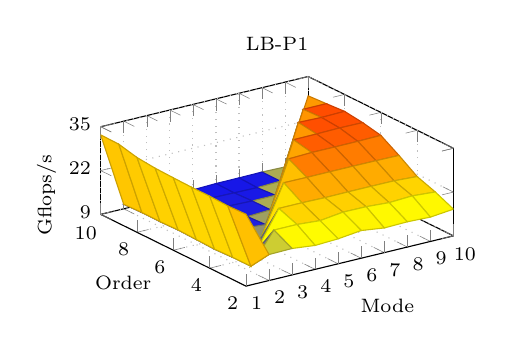
\begin{tikzpicture}
\begin{axis}[height=0.35\textwidth,width=0.5\textwidth,style={font=\scriptsize},grid=major,grid style={dotted},align=center,xlabel={Mode}, ylabel={Order},zlabel={Gflops/s},title={\ttt{LB-P1}}, xtick={1,2,3,4,5,6,7,8,9,10},xticklabels={1,2,3,4,5,6,7,8,9,10}, ytick={2,4,6,8,10}, yticklabels={2,4,6,8,10}, point meta max=35, point meta min=9, zmin=9, zmax=35, ztick={9,22,35}, zticklabels={9,22,35}, view={-35}{45}, xlabel style={yshift=2mm}, ylabel style={yshift=4mm}, zlabel style={yshift=-1mm,xshift=-4mm}]
\addplot3[surf] %, colormap = {whiteblack}{color(0cm)=(white);color(0.4cm) = (darkgray)}
coordinates{
(1.000,2.000,30.340) (1.000,3.000,30.150) (1.000,4.000,30.377) (1.000,5.000,30.377) (1.000,6.000,30.496) (1.000,7.000,30.686) (1.000,8.000,31.196) (1.000,9.000,32.484) (1.000,10.000,32.591) 
	
(2.000,2.000,16.722) (2.000,3.000,10.585) (2.000,4.000,10.550) (2.000,5.000,10.314) (2.000,6.000,10.511) (2.000,7.000,10.673) (2.000,8.000,10.503) (2.000,9.000,10.548) (2.000,10.000,10.332) 

(3.000,2.000,16.857) (3.000,3.000,19.659) (3.000,4.000,10.526) (3.000,5.000,10.205) (3.000,6.000,10.288) (3.000,7.000,10.147) (3.000,8.000,10.260) (3.000,9.000,9.797) (3.000,10.000,10.055) 

(4.000,2.000,16.102) (4.000,3.000,19.651) (4.000,4.000,21.764) (4.000,5.000,10.137) (4.000,6.000,10.555) (4.000,7.000,10.015) (4.000,8.000,10.299) (4.000,9.000,10.105) (4.000,10.000,9.908) 

(5.000,2.000,16.414) (5.000,3.000,19.135) (5.000,4.000,21.771) (5.000,5.000,25.061) (5.000,6.000,9.984) (5.000,7.000,9.693) (5.000,8.000,10.201) (5.000,9.000,9.856) (5.000,10.000,9.636) 

(6.000,2.000,17.213) (6.000,3.000,20.011) (6.000,4.000,21.633) (6.000,5.000,24.989) (6.000,6.000,27.821) (6.000,7.000,10.053) (6.000,8.000,10.014) (6.000,9.000,9.749) (6.000,10.000,9.862) 

(7.000,2.000,16.320) (7.000,3.000,19.956) (7.000,4.000,21.696) (7.000,5.000,25.002) (7.000,6.000,28.062) (7.000,7.000,29.186) (7.000,8.000,10.048) (7.000,9.000,9.639) (7.000,10.000,9.882) 
	
(8.000,2.000,16.492) (8.000,3.000,19.515) (8.000,4.000,21.696) (8.000,5.000,25.000) (8.000,6.000,28.036) (8.000,7.000,29.241) (8.000,8.000,30.006) (8.000,9.000,9.911) (8.000,10.000,9.964) 
	
(9.000,2.000,16.228) (9.000,3.000,19.860) (9.000,4.000,21.672) (9.000,5.000,24.976) (9.000,6.000,28.062) (9.000,7.000,29.371) (9.000,8.000,29.826) (9.000,9.000,29.590) (9.000,10.000,9.821) 
	
(10.000,2.000,16.926) (10.000,3.000,19.364) (10.000,4.000,21.283) (10.000,5.000,24.884) (10.000,6.000,28.180) (10.000,7.000,29.297) (10.000,8.000,29.988) (10.000,9.000,29.598) (10.000,10.000,29.257) 
	
};\end{axis}
\end{tikzpicture}
\begin{comment}
\begin{tikzpicture}
\begin{axis}[height=0.40\textheight,width=0.40\textwidth,style={font=\footnotesize},grid=major,grid style={dotted},align=center,xlabel={Kontraktionsmodus},ylabel={Tensorstufe},title={{LB}-{P1}},scaled ticks=false,zticklabel=\pgfmathprintnumber{\tick},zlabel={Durchsatz [Gflops/s]},view={-45}{45}, zlabel={Standardfehler [\%]}]
\addplot3[surf]
coordinates{(1.000,2.000,1.865) (1.000,3.000,2.919) (1.000,4.000,3.127) (1.000,5.000,3.522) (1.000,6.000,4.168) (1.000,7.000,4.511) (1.000,8.000,4.143) (1.000,9.000,1.151) (1.000,10.000,1.071) 
	
	(2.000,2.000,1.262) (2.000,3.000,9.168) (2.000,4.000,12.462) (2.000,5.000,10.166) (2.000,6.000,11.619) (2.000,7.000,11.462) (2.000,8.000,10.765) (2.000,9.000,11.361) (2.000,10.000,11.626) 
	
	(3.000,2.000,4.592) (3.000,3.000,1.071) (3.000,4.000,8.620) (3.000,5.000,11.768) (3.000,6.000,8.149) (3.000,7.000,11.048) (3.000,8.000,12.646) (3.000,9.000,10.426) (3.000,10.000,11.319) 
	
	(4.000,2.000,2.505) (4.000,3.000,0.801) (4.000,4.000,1.578) (4.000,5.000,11.887) (4.000,6.000,12.483) (4.000,7.000,10.515) (4.000,8.000,8.651) (4.000,9.000,12.485) (4.000,10.000,12.117) 
	
	(5.000,2.000,3.123) (5.000,3.000,1.145) (5.000,4.000,1.532) (5.000,5.000,2.987) (5.000,6.000,11.781) (5.000,7.000,11.819) (5.000,8.000,9.498) (5.000,9.000,11.849) (5.000,10.000,11.091) 
	
	(6.000,2.000,3.540) (6.000,3.000,1.277) (6.000,4.000,1.801) (6.000,5.000,2.805) (6.000,6.000,2.525) (6.000,7.000,8.015) (6.000,8.000,13.387) (6.000,9.000,8.782) (6.000,10.000,10.696) 
	
	(7.000,2.000,3.614) (7.000,3.000,1.138) (7.000,4.000,1.704) (7.000,5.000,2.909) (7.000,6.000,2.451) (7.000,7.000,1.946) (7.000,8.000,11.372) (7.000,9.000,11.030) (7.000,10.000,12.054) 
	
	(8.000,2.000,4.086) (8.000,3.000,1.392) (8.000,4.000,1.646) (8.000,5.000,3.144) (8.000,6.000,2.326) (8.000,7.000,1.922) (8.000,8.000,1.426) (8.000,9.000,10.847) (8.000,10.000,9.075) 
	
	(9.000,2.000,3.670) (9.000,3.000,1.277) (9.000,4.000,1.418) (9.000,5.000,2.937) (9.000,6.000,2.300) (9.000,7.000,1.882) (9.000,8.000,1.527) (9.000,9.000,0.967) (9.000,10.000,10.730) 
	
	(10.000,2.000,3.497) (10.000,3.000,1.058) (10.000,4.000,1.789) (10.000,5.000,3.050) (10.000,6.000,2.069) (10.000,7.000,1.794) (10.000,8.000,1.428) (10.000,9.000,0.969) (10.000,10.000,0.529) 
	
};\end{axis}
\end{tikzpicture}
\end{comment}
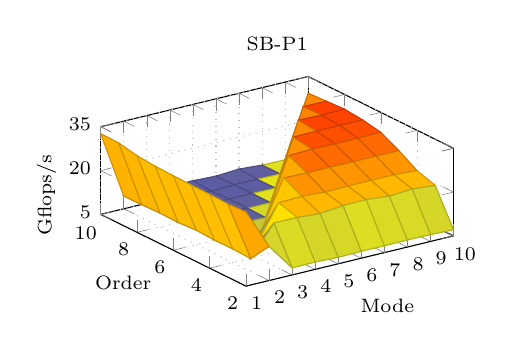
\begin{tikzpicture}
\begin{axis}[height=0.35\textwidth,width=0.5\textwidth,style={font=\scriptsize},grid=major,grid style={dotted},align=center,xlabel={Mode},ylabel={Order},zlabel={Gflops/s},title={\ttt{SB-P1}}, xtick={1,2,3,4,5,6,7,8,9,10},xticklabels={1,2,3,4,5,6,7,8,9,10}, ytick={2,4,6,8,10}, yticklabels={2,4,6,8,10}, point meta max=35, point meta min=5, zmin=5, zmax=35, ztick={5,20,35}, zticklabels={5,20,35}, view={-35}{45}, xlabel style={yshift=2mm}, ylabel style={yshift=4mm}, zlabel style={yshift=-1mm,xshift=-4mm}]
\addplot3[surf] % , colormap = {whiteblack}{color(0cm)=(white);color(0.4cm) = (darkgray)}
coordinates{
(1.000,2.000,30.432) (1.000,3.000,30.105) (1.000,4.000,30.292) (1.000,5.000,30.361) (1.000,6.000,30.537) (1.000,7.000,30.721) (1.000,8.000,31.253) (1.000,9.000,32.509) (1.000,10.000,32.643) 

(2.000,2.000,16.708) (2.000,3.000,9.472) (2.000,4.000,9.724) (2.000,5.000,9.652) (2.000,6.000,9.963) (2.000,7.000,9.546) (2.000,8.000,9.694) (2.000,9.000,9.463) (2.000,10.000,9.405) 

(3.000,2.000,7.397) (3.000,3.000,19.720) (3.000,4.000,8.618) (3.000,5.000,9.043) (3.000,6.000,9.168) (3.000,7.000,9.161) (3.000,8.000,8.551) (3.000,9.000,8.307) (3.000,10.000,8.404) 

(4.000,2.000,7.495) (4.000,3.000,19.656) (4.000,4.000,21.706) (4.000,5.000,8.562) (4.000,6.000,8.778) (4.000,7.000,8.882) (4.000,8.000,8.704) (4.000,9.000,8.760) (4.000,10.000,8.724) 

(5.000,2.000,7.187) (5.000,3.000,19.134) (5.000,4.000,21.919) (5.000,5.000,25.134) (5.000,6.000,8.534) (5.000,7.000,8.679) (5.000,8.000,8.767) (5.000,9.000,8.350) (5.000,10.000,8.891) 

(6.000,2.000,7.370) (6.000,3.000,19.899) (6.000,4.000,21.481) (6.000,5.000,24.987) (6.000,6.000,27.823) (6.000,7.000,8.658) (6.000,8.000,8.711) (6.000,9.000,8.624) (6.000,10.000,8.539) 

(7.000,2.000,7.310) (7.000,3.000,20.082) (7.000,4.000,21.602) (7.000,5.000,24.982) (7.000,6.000,28.118) (7.000,7.000,29.190) (7.000,8.000,8.681) (7.000,9.000,8.601) (7.000,10.000,9.051) 

(8.000,2.000,7.424) (8.000,3.000,19.351) (8.000,4.000,21.686) (8.000,5.000,24.979) (8.000,6.000,28.026) (8.000,7.000,29.333) (8.000,8.000,30.003) (8.000,9.000,8.518) (8.000,10.000,8.490) 

(9.000,2.000,7.317) (9.000,3.000,19.880) (9.000,4.000,21.646) (9.000,5.000,24.979) (9.000,6.000,28.078) (9.000,7.000,29.364) (9.000,8.000,29.802) (9.000,9.000,29.655) (9.000,10.000,8.382) 

(10.000,2.000,7.117) (10.000,3.000,19.176) (10.000,4.000,21.198) (10.000,5.000,24.958) (10.000,6.000,28.156) (10.000,7.000,29.342) (10.000,8.000,29.950) (10.000,9.000,29.630) (10.000,10.000,29.294) 

};
\end{axis}
\end{tikzpicture}
\begin{comment}
\begin{tikzpicture}
\begin{axis}[height=0.40\textheight,width=0.40\textwidth,style={font=\footnotesize},grid=major,grid style={dotted},align=center,xlabel={Kontraktionsmodus},ylabel={Tensorstufe},title={TLib-SB-{P1}},scaled ticks=false,zticklabel=\pgfmathprintnumber{\tick},zlabel={Durchsatz [Gflops/s]},view={-45}{45}, zlabel={Standardfehler [\%]}]
\addplot3[surf]
coordinates{(1.000,2.000,2.166) (1.000,3.000,2.892) (1.000,4.000,3.520) (1.000,5.000,3.679) (1.000,6.000,4.069) (1.000,7.000,4.572) (1.000,8.000,4.220) (1.000,9.000,1.113) (1.000,10.000,0.757) 

(2.000,2.000,1.392) (2.000,3.000,12.181) (2.000,4.000,11.639) (2.000,5.000,12.297) (2.000,6.000,13.483) (2.000,7.000,11.327) (2.000,8.000,11.608) (2.000,9.000,10.021) (2.000,10.000,7.762) 

(3.000,2.000,0.605) (3.000,3.000,0.922) (3.000,4.000,7.262) (3.000,5.000,11.507) (3.000,6.000,10.980) (3.000,7.000,13.088) (3.000,8.000,10.499) (3.000,9.000,7.891) (3.000,10.000,10.541) 

(4.000,2.000,1.318) (4.000,3.000,0.895) (4.000,4.000,1.614) (4.000,5.000,11.723) (4.000,6.000,10.371) (4.000,7.000,10.552) (4.000,8.000,10.448) (4.000,9.000,11.639) (4.000,10.000,9.715) 

(5.000,2.000,0.444) (5.000,3.000,1.269) (5.000,4.000,1.329) (5.000,5.000,2.894) (5.000,6.000,12.131) (5.000,7.000,9.577) (5.000,8.000,12.183) (5.000,9.000,10.336) (5.000,10.000,9.377) 

(6.000,2.000,0.484) (6.000,3.000,1.237) (6.000,4.000,2.109) (6.000,5.000,2.884) (6.000,6.000,2.497) (6.000,7.000,11.915) (6.000,8.000,10.138) (6.000,9.000,10.479) (6.000,10.000,7.941) 

(7.000,2.000,0.432) (7.000,3.000,0.895) (7.000,4.000,1.727) (7.000,5.000,3.155) (7.000,6.000,2.530) (7.000,7.000,2.054) (7.000,8.000,9.984) (7.000,9.000,9.380) (7.000,10.000,9.855) 

(8.000,2.000,0.914) (8.000,3.000,1.192) (8.000,4.000,1.724) (8.000,5.000,3.100) (8.000,6.000,2.479) (8.000,7.000,1.911) (8.000,8.000,1.571) (8.000,9.000,8.906) (8.000,10.000,9.600) 

(9.000,2.000,0.373) (9.000,3.000,1.424) (9.000,4.000,1.392) (9.000,5.000,2.961) (9.000,6.000,2.325) (9.000,7.000,1.999) (9.000,8.000,1.713) (9.000,9.000,1.236) (9.000,10.000,8.944) 

(10.000,2.000,0.397) (10.000,3.000,1.321) (10.000,4.000,1.594) (10.000,5.000,3.096) (10.000,6.000,2.287) (10.000,7.000,1.961) (10.000,8.000,1.488) (10.000,9.000,0.959) (10.000,10.000,0.535) 

};\end{axis}
\end{tikzpicture}
\end{comment}

%%%%%%%%%%%%%%%%%%%%%%%%%%%

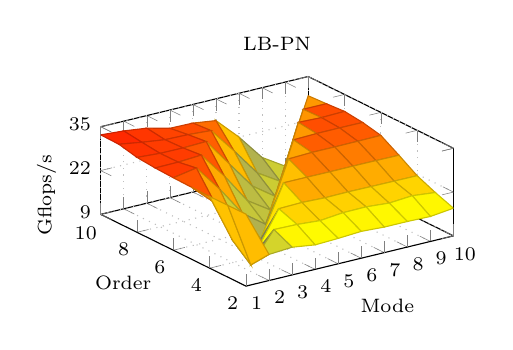
\begin{tikzpicture}
\begin{axis}[height=0.35\textwidth,width=0.5\textwidth,style={font=\scriptsize},grid=major,grid style={dotted},align=center,xlabel={Mode},ylabel={Order},zlabel={Gflops/s},title={\ttt{LB-PN}}, xtick={1,2,3,4,5,6,7,8,9,10},xticklabels={1,2,3,4,5,6,7,8,9,10}, ytick={2,4,6,8,10}, yticklabels={2,4,6,8,10}, point meta max=35, point meta min=9, zmin=9, zmax=35, ztick={9,22,35}, zticklabels={9,22,35}, view={-35}{45}, xlabel style={yshift=2mm}, ylabel style={yshift=4mm}, zlabel style={yshift=-1mm,xshift=-4mm}]
\addplot3[surf] %, colormap = {whiteblack}{color(0cm)=(white);color(0.4cm) = (darkgray)}
coordinates{
(1.000,2.000,30.353) (1.000,3.000,30.312) (1.000,4.000,30.265) (1.000,5.000,30.361) (1.000,6.000,30.506) (1.000,7.000,30.751) (1.000,8.000,31.224) (1.000,9.000,32.470) (1.000,10.000,32.590) 

(2.000,2.000,16.748) (2.000,3.000,10.971) (2.000,4.000,15.539) (2.000,5.000,24.166) (2.000,6.000,31.744) (2.000,7.000,30.820) (2.000,8.000,30.771) (2.000,9.000,31.394) (2.000,10.000,32.110) 

(3.000,2.000,17.232) (3.000,3.000,19.809) (3.000,4.000,10.343) (3.000,5.000,15.135) (3.000,6.000,23.893) (3.000,7.000,31.252) (3.000,8.000,30.718) (3.000,9.000,30.505) (3.000,10.000,31.268) 

(4.000,2.000,16.270) (4.000,3.000,19.656) (4.000,4.000,21.676) (4.000,5.000,9.964) (4.000,6.000,14.975) (4.000,7.000,23.383) (4.000,8.000,30.969) (4.000,9.000,30.341) (4.000,10.000,29.576) 

(5.000,2.000,16.531) (5.000,3.000,19.141) (5.000,4.000,21.867) (5.000,5.000,25.058) (5.000,6.000,10.071) (5.000,7.000,14.425) (5.000,8.000,22.690) (5.000,9.000,29.897) (5.000,10.000,29.463) 

(6.000,2.000,16.960) (6.000,3.000,19.837) (6.000,4.000,21.600) (6.000,5.000,25.039) (6.000,6.000,27.817) (6.000,7.000,9.995) (6.000,8.000,14.451) (6.000,9.000,22.192) (6.000,10.000,28.544) 

(7.000,2.000,16.580) (7.000,3.000,19.918) (7.000,4.000,21.691) (7.000,5.000,24.989) (7.000,6.000,28.077) (7.000,7.000,29.165) (7.000,8.000,9.692) (7.000,9.000,14.040) (7.000,10.000,21.983) 

(8.000,2.000,16.580) (8.000,3.000,19.375) (8.000,4.000,21.619) (8.000,5.000,25.026) (8.000,6.000,28.052) (8.000,7.000,29.365) (8.000,8.000,30.029) (8.000,9.000,9.851) (8.000,10.000,14.291) 

(9.000,2.000,16.414) (9.000,3.000,19.905) (9.000,4.000,21.575) (9.000,5.000,25.011) (9.000,6.000,28.093) (9.000,7.000,29.394) (9.000,8.000,29.785) (9.000,9.000,29.598) (9.000,10.000,10.064) 

(10.000,2.000,17.212) (10.000,3.000,19.196) (10.000,4.000,21.529) (10.000,5.000,24.939) (10.000,6.000,28.175) (10.000,7.000,29.346) (10.000,8.000,29.977) (10.000,9.000,29.587) (10.000,10.000,29.286) 

};
\end{axis}
\end{tikzpicture}
\begin{comment}
\begin{tikzpicture}
\begin{axis}[height=0.40\textheight,width=0.40\textwidth,style={font=\footnotesize},grid=major,grid style={dotted},align=center,xlabel={Kontraktionsmodus},ylabel={Tensorstufe},title={TLib-{LB}-{P2}},scaled ticks=false,zticklabel=\pgfmathprintnumber{\tick},zlabel={Durchsatz [Gflops/s]},view={-45}{45}, zlabel={Standardfehler [\%]}]
\addplot3[surf]
coordinates{(1.000,2.000,1.898) (1.000,3.000,2.533) (1.000,4.000,3.595) (1.000,5.000,3.637) (1.000,6.000,4.113) (1.000,7.000,4.502) (1.000,8.000,4.207) (1.000,9.000,1.266) (1.000,10.000,0.884) 

(2.000,2.000,1.169) (2.000,3.000,11.043) (2.000,4.000,6.645) (2.000,5.000,2.391) (2.000,6.000,1.025) (2.000,7.000,4.511) (2.000,8.000,1.619) (2.000,9.000,0.693) (2.000,10.000,0.822) 

(3.000,2.000,1.320) (3.000,3.000,0.851) (3.000,4.000,9.683) (3.000,5.000,5.843) (3.000,6.000,3.221) (3.000,7.000,1.216) (3.000,8.000,0.984) (3.000,9.000,1.380) (3.000,10.000,1.076) 

(4.000,2.000,1.325) (4.000,3.000,0.745) (4.000,4.000,1.694) (4.000,5.000,11.366) (4.000,6.000,6.330) (4.000,7.000,3.547) (4.000,8.000,0.999) (4.000,9.000,1.225) (4.000,10.000,1.703) 

(5.000,2.000,1.246) (5.000,3.000,1.437) (5.000,4.000,1.529) (5.000,5.000,3.048) (5.000,6.000,11.659) (5.000,7.000,4.919) (5.000,8.000,2.871) (5.000,9.000,1.048) (5.000,10.000,0.939) 

(6.000,2.000,1.029) (6.000,3.000,2.674) (6.000,4.000,1.744) (6.000,5.000,2.929) (6.000,6.000,2.549) (6.000,7.000,11.158) (6.000,8.000,7.762) (6.000,9.000,2.713) (6.000,10.000,2.683) 

(7.000,2.000,1.531) (7.000,3.000,1.399) (7.000,4.000,1.550) (7.000,5.000,3.221) (7.000,6.000,2.580) (7.000,7.000,2.115) (7.000,8.000,11.269) (7.000,9.000,5.413) (7.000,10.000,2.656) 

(8.000,2.000,1.175) (8.000,3.000,1.232) (8.000,4.000,1.688) (8.000,5.000,3.296) (8.000,6.000,2.418) (8.000,7.000,1.947) (8.000,8.000,1.461) (8.000,9.000,11.645) (8.000,10.000,6.477) 

(9.000,2.000,1.615) (9.000,3.000,1.306) (9.000,4.000,1.865) (9.000,5.000,2.913) (9.000,6.000,2.408) (9.000,7.000,1.971) (9.000,8.000,1.681) (9.000,9.000,1.046) (9.000,10.000,8.565) 

(10.000,2.000,1.005) (10.000,3.000,1.219) (10.000,4.000,1.467) (10.000,5.000,3.104) (10.000,6.000,2.206) (10.000,7.000,1.980) (10.000,8.000,1.611) (10.000,9.000,1.052) (10.000,10.000,0.601) 

};
\end{axis}
\end{tikzpicture}
\end{comment}
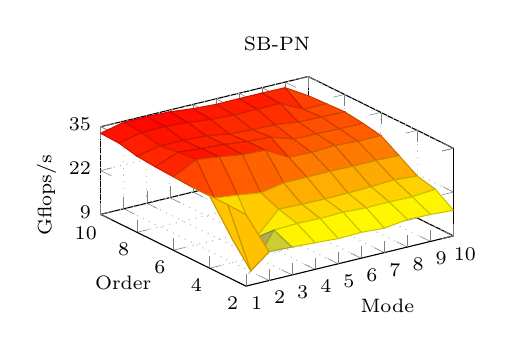
\begin{tikzpicture}
\begin{axis}[height=0.35\textwidth,width=0.5\textwidth,style={font=\scriptsize},grid=major,grid style={dotted},align=center,xlabel={Mode},ylabel={Order},zlabel={Gflops/s},title={\ttt{SB-PN}}, xtick={1,2,3,4,5,6,7,8,9,10},xticklabels={1,2,3,4,5,6,7,8,9,10}, ytick={2,4,6,8,10}, yticklabels={2,4,6,8,10}, point meta max=35, point meta min=9, zmin=9, zmax=35, ztick={9,22,35}, zticklabels={9,22,35}, view={-35}{45}, xlabel style={yshift=2mm}, ylabel style={yshift=4mm}, zlabel style={yshift=-1mm,xshift=-4mm}]
\addplot3[surf] % , colormap = {whiteblack}{color(0cm)=(white);color(0.4cm) = (darkgray)}
coordinates{
(1.000,2.000,30.244) (1.000,3.000,30.448) (1.000,4.000,30.513) (1.000,5.000,30.521) (1.000,6.000,30.805) (1.000,7.000,31.123) (1.000,8.000,31.582) (1.000,9.000,32.837) (1.000,10.000,33.056) 

(2.000,2.000,17.544) (2.000,3.000,9.230) (2.000,4.000,15.792) (2.000,5.000,25.482) (2.000,6.000,34.267) (2.000,7.000,33.761) (2.000,8.000,32.969) (2.000,9.000,34.257) (2.000,10.000,34.664) 

(3.000,2.000,17.291) (3.000,3.000,19.621) (3.000,4.000,14.674) (3.000,5.000,24.720) (3.000,6.000,33.420) (3.000,7.000,33.220) (3.000,8.000,32.935) (3.000,9.000,34.433) (3.000,10.000,34.713) 

(4.000,2.000,16.905) (4.000,3.000,19.948) (4.000,4.000,21.543) (4.000,5.000,23.741) (4.000,6.000,32.390) (4.000,7.000,32.790) (4.000,8.000,32.688) (4.000,9.000,33.939) (4.000,10.000,34.455) 

(5.000,2.000,16.491) (5.000,3.000,19.785) (5.000,4.000,21.325) (5.000,5.000,25.035) (5.000,6.000,32.072) (5.000,7.000,31.950) (5.000,8.000,31.519) (5.000,9.000,33.185) (5.000,10.000,33.743) 

(6.000,2.000,16.671) (6.000,3.000,19.953) (6.000,4.000,21.260) (6.000,5.000,25.077) (6.000,6.000,28.310) (6.000,7.000,31.655) (6.000,8.000,31.193) (6.000,9.000,32.836) (6.000,10.000,33.351) 

(7.000,2.000,16.269) (7.000,3.000,19.634) (7.000,4.000,21.358) (7.000,5.000,25.149) (7.000,6.000,28.067) (7.000,7.000,29.384) (7.000,8.000,30.938) (7.000,9.000,32.937) (7.000,10.000,33.399) 

(8.000,2.000,17.174) (8.000,3.000,19.698) (8.000,4.000,21.570) (8.000,5.000,25.007) (8.000,6.000,28.450) (8.000,7.000,29.241) (8.000,8.000,30.115) (8.000,9.000,32.937) (8.000,10.000,33.406) 

(9.000,2.000,16.998) (9.000,3.000,19.599) (9.000,4.000,21.975) (9.000,5.000,25.064) (9.000,6.000,28.078) (9.000,7.000,29.100) (9.000,8.000,29.960) (9.000,9.000,29.632) (9.000,10.000,33.336) 

(10.000,2.000,16.611) (10.000,3.000,20.174) (10.000,4.000,21.453) (10.000,5.000,24.861) (10.000,6.000,28.132) (10.000,7.000,29.142) (10.000,8.000,29.866) (10.000,9.000,29.588) (10.000,10.000,29.300) 

};\end{axis}
\end{tikzpicture}
\begin{comment}
\begin{tikzpicture}
\begin{axis}[height=0.40\textheight,width=0.40\textwidth,style={font=\footnotesize},grid=major,grid style={dotted},align=center,xlabel={Kontraktionsmodus},ylabel={Tensorstufe},title={TLib-SB-PB3},scaled ticks=false,zticklabel=\pgfmathprintnumber{\tick},zlabel={Durchsatz [Gflops/s]},view={-45}{45}, zlabel={Standardfehler [\%]}]
\addplot3[surf]
coordinates{(1.000,2.000,4.915) (1.000,3.000,2.617) (1.000,4.000,3.193) (1.000,5.000,4.037) (1.000,6.000,4.649) (1.000,7.000,4.045) (1.000,8.000,4.268) (1.000,9.000,1.298) (1.000,10.000,0.649) 

(2.000,2.000,1.146) (2.000,3.000,12.575) (2.000,4.000,10.226) (2.000,5.000,3.407) (2.000,6.000,1.272) (2.000,7.000,1.332) (2.000,8.000,1.219) (2.000,9.000,0.793) (2.000,10.000,0.947) 

(3.000,2.000,1.573) (3.000,3.000,1.382) (3.000,4.000,6.180) (3.000,5.000,3.661) (3.000,6.000,2.150) (3.000,7.000,1.692) (3.000,8.000,0.904) (3.000,9.000,0.674) (3.000,10.000,1.161) 

(4.000,2.000,2.256) (4.000,3.000,1.618) (4.000,4.000,1.501) (4.000,5.000,1.999) (4.000,6.000,1.755) (4.000,7.000,1.631) (4.000,8.000,1.231) (4.000,9.000,0.488) (4.000,10.000,0.991) 

(5.000,2.000,2.165) (5.000,3.000,1.481) (5.000,4.000,1.653) (5.000,5.000,2.982) (5.000,6.000,2.611) (5.000,7.000,2.199) (5.000,8.000,1.877) (5.000,9.000,0.945) (5.000,10.000,0.484) 

(6.000,2.000,1.881) (6.000,3.000,1.437) (6.000,4.000,1.837) (6.000,5.000,2.992) (6.000,6.000,2.179) (6.000,7.000,3.249) (6.000,8.000,2.066) (6.000,9.000,1.171) (6.000,10.000,0.683) 

(7.000,2.000,1.280) (7.000,3.000,1.511) (7.000,4.000,1.790) (7.000,5.000,2.757) (7.000,6.000,2.313) (7.000,7.000,2.193) (7.000,8.000,1.944) (7.000,9.000,1.215) (7.000,10.000,0.680) 

(8.000,2.000,2.513) (8.000,3.000,1.442) (8.000,4.000,1.953) (8.000,5.000,2.795) (8.000,6.000,2.272) (8.000,7.000,2.173) (8.000,8.000,1.382) (8.000,9.000,1.317) (8.000,10.000,0.759) 

(9.000,2.000,2.432) (9.000,3.000,1.826) (9.000,4.000,1.406) (9.000,5.000,2.650) (9.000,6.000,2.476) (9.000,7.000,2.317) (9.000,8.000,1.006) (9.000,9.000,1.365) (9.000,10.000,0.782) 

(10.000,2.000,2.422) (10.000,3.000,1.313) (10.000,4.000,2.697) (10.000,5.000,2.971) (10.000,6.000,2.301) (10.000,7.000,1.950) (10.000,8.000,1.294) (10.000,9.000,1.121) (10.000,10.000,0.678) 

};\end{axis}
\end{tikzpicture}
\end{comment}

\caption{%
\footnotesize %
Average performance maps of four tensor-vector multiplications with varying tensor orders $p$  and contraction modes $q$.		
Tensor elements are encoded in single-precision and stored contiguously in memory according to the first-order storage format.
Tensors are \tit{asymmetrically}-\tit{shaped} with dimensions.
%Arithmetic mean is calculated over the tensor size.
\label{performance.tlib.sb.lb.order1.single.surf.nonsymmetric}
}
\end{figure*}
\begin{comment}
\begin{figure*}[t]
	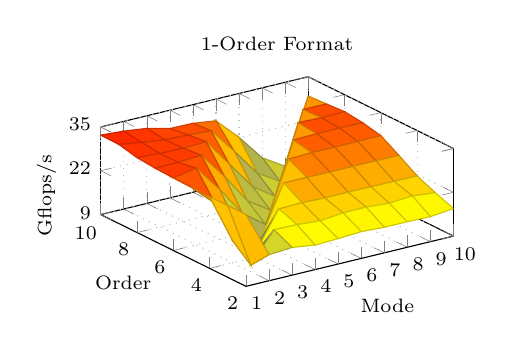
\begin{tikzpicture}
\begin{axis}[height=0.35\textwidth,width=0.5\textwidth,style={font=\scriptsize},grid=major,grid style={dotted},align=center,xlabel={Mode},ylabel={Order},zlabel={Gflops/s},title={$1$-Order Format}, xtick={1,2,3,4,5,6,7,8,9,10},xticklabels={1,2,3,4,5,6,7,8,9,10}, ytick={2,4,6,8,10}, yticklabels={2,4,6,8,10}, point meta max=35, point meta min=9, zmin=9, zmax=35, ztick={9,22,35},zticklabels={9,22,35}, view={-35}{45}, xlabel style={yshift=2mm}, ylabel style={yshift=4mm}, zlabel style={yshift=-1mm,xshift=-4mm}]
\addplot3[surf] %,colormap = {whiteblack}{color(0cm)=(white);color(0.4cm) = (darkgray)}
coordinates{
(1.000,2.000,30.353) (1.000,3.000,30.312) (1.000,4.000,30.265) (1.000,5.000,30.361) (1.000,6.000,30.506) (1.000,7.000,30.751) (1.000,8.000,31.224) (1.000,9.000,32.470) (1.000,10.000,32.590) 

(2.000,2.000,16.748) (2.000,3.000,10.971) (2.000,4.000,15.539) (2.000,5.000,24.166) (2.000,6.000,31.744) (2.000,7.000,30.820) (2.000,8.000,30.771) (2.000,9.000,31.394) (2.000,10.000,32.110) 

(3.000,2.000,17.232) (3.000,3.000,19.809) (3.000,4.000,10.343) (3.000,5.000,15.135) (3.000,6.000,23.893) (3.000,7.000,31.252) (3.000,8.000,30.718) (3.000,9.000,30.505) (3.000,10.000,31.268) 

(4.000,2.000,16.270) (4.000,3.000,19.656) (4.000,4.000,21.676) (4.000,5.000,9.964) (4.000,6.000,14.975) (4.000,7.000,23.383) (4.000,8.000,30.969) (4.000,9.000,30.341) (4.000,10.000,29.576) 

(5.000,2.000,16.531) (5.000,3.000,19.141) (5.000,4.000,21.867) (5.000,5.000,25.058) (5.000,6.000,10.071) (5.000,7.000,14.425) (5.000,8.000,22.690) (5.000,9.000,29.897) (5.000,10.000,29.463) 

(6.000,2.000,16.960) (6.000,3.000,19.837) (6.000,4.000,21.600) (6.000,5.000,25.039) (6.000,6.000,27.817) (6.000,7.000,9.995) (6.000,8.000,14.451) (6.000,9.000,22.192) (6.000,10.000,28.544) 

(7.000,2.000,16.580) (7.000,3.000,19.918) (7.000,4.000,21.691) (7.000,5.000,24.989) (7.000,6.000,28.077) (7.000,7.000,29.165) (7.000,8.000,9.692) (7.000,9.000,14.040) (7.000,10.000,21.983) 

(8.000,2.000,16.580) (8.000,3.000,19.375) (8.000,4.000,21.619) (8.000,5.000,25.026) (8.000,6.000,28.052) (8.000,7.000,29.365) (8.000,8.000,30.029) (8.000,9.000,9.851) (8.000,10.000,14.291) 

(9.000,2.000,16.414) (9.000,3.000,19.905) (9.000,4.000,21.575) (9.000,5.000,25.011) (9.000,6.000,28.093) (9.000,7.000,29.394) (9.000,8.000,29.785) (9.000,9.000,29.598) (9.000,10.000,10.064) 

(10.000,2.000,17.212) (10.000,3.000,19.196) (10.000,4.000,21.529) (10.000,5.000,24.939) (10.000,6.000,28.175) (10.000,7.000,29.346) (10.000,8.000,29.977) (10.000,9.000,29.587) (10.000,10.000,29.286) 

};
\end{axis}
\end{tikzpicture}
\begin{comment}
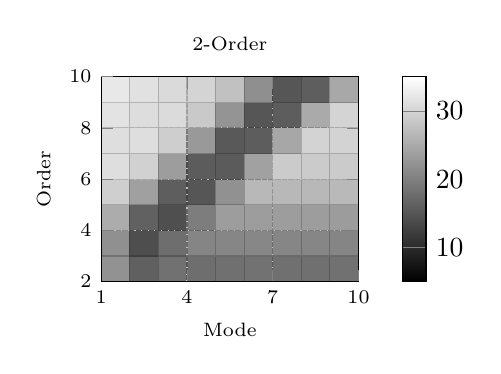
\begin{tikzpicture}
\begin{axis}[width=0.40\textwidth,style={font=\scriptsize},grid=major,grid style={dotted},align=center,xlabel={Mode},ylabel={Order},zlabel={Gflops/s},title={2-Order}, xtick={1,4,7,10},xticklabels={1,4,7,10}, ytick={2,4,6,8,10}, yticklabels={2,4,6,8,10}, point meta max=35, point meta min=5, ztick={5,15,25,35},zticklabels={5,15,25,35}, view={0}{90}, colorbar,colormap/blackwhite, colorbar style={width=0.3cm}]
\addplot3[surf] %  colormap/blackwhite ,shader=faceted interp, colormap = {whiteblack}{color(0cm)=(white);color(0.4cm) = (darkgray)}
coordinates{(1.000,2.000,30.353) (1.000,3.000,30.312) (1.000,4.000,30.265) (1.000,5.000,30.361) (1.000,6.000,30.506) (1.000,7.000,30.751) (1.000,8.000,31.224) (1.000,9.000,32.470) (1.000,10.000,32.590) 

(2.000,2.000,16.748) (2.000,3.000,10.971) (2.000,4.000,15.539) (2.000,5.000,24.166) (2.000,6.000,31.744) (2.000,7.000,30.820) (2.000,8.000,30.771) (2.000,9.000,31.394) (2.000,10.000,32.110) 

(3.000,2.000,17.232) (3.000,3.000,19.809) (3.000,4.000,10.343) (3.000,5.000,15.135) (3.000,6.000,23.893) (3.000,7.000,31.252) (3.000,8.000,30.718) (3.000,9.000,30.505) (3.000,10.000,31.268) 

(4.000,2.000,16.270) (4.000,3.000,19.656) (4.000,4.000,21.676) (4.000,5.000,9.964) (4.000,6.000,14.975) (4.000,7.000,23.383) (4.000,8.000,30.969) (4.000,9.000,30.341) (4.000,10.000,29.576) 

(5.000,2.000,16.531) (5.000,3.000,19.141) (5.000,4.000,21.867) (5.000,5.000,25.058) (5.000,6.000,10.071) (5.000,7.000,14.425) (5.000,8.000,22.690) (5.000,9.000,29.897) (5.000,10.000,29.463) 

(6.000,2.000,16.960) (6.000,3.000,19.837) (6.000,4.000,21.600) (6.000,5.000,25.039) (6.000,6.000,27.817) (6.000,7.000,9.995) (6.000,8.000,14.451) (6.000,9.000,22.192) (6.000,10.000,28.544) 

(7.000,2.000,16.580) (7.000,3.000,19.918) (7.000,4.000,21.691) (7.000,5.000,24.989) (7.000,6.000,28.077) (7.000,7.000,29.165) (7.000,8.000,9.692) (7.000,9.000,14.040) (7.000,10.000,21.983) 

(8.000,2.000,16.580) (8.000,3.000,19.375) (8.000,4.000,21.619) (8.000,5.000,25.026) (8.000,6.000,28.052) (8.000,7.000,29.365) (8.000,8.000,30.029) (8.000,9.000,9.851) (8.000,10.000,14.291) 

(9.000,2.000,16.414) (9.000,3.000,19.905) (9.000,4.000,21.575) (9.000,5.000,25.011) (9.000,6.000,28.093) (9.000,7.000,29.394) (9.000,8.000,29.785) (9.000,9.000,29.598) (9.000,10.000,10.064) 

(10.000,2.000,17.212) (10.000,3.000,19.196) (10.000,4.000,21.529) (10.000,5.000,24.939) (10.000,6.000,28.175) (10.000,7.000,29.346) (10.000,8.000,29.977) (10.000,9.000,29.587) (10.000,10.000,29.286) 

};
\end{axis}
\end{tikzpicture}
\end{comment}
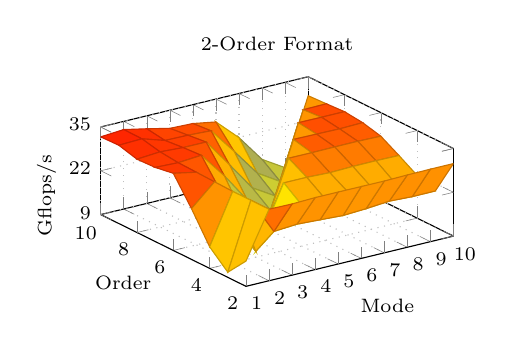
\begin{tikzpicture}
\begin{axis}[height=0.35\textwidth,width=0.5\textwidth,style={font=\scriptsize},grid=major,grid style={dotted},align=center,xlabel={Mode},ylabel={Order},zlabel={Gflops/s},title={$2$-Order Format}, xtick={1,2,3,4,5,6,7,8,9,10},xticklabels={1,2,3,4,5,6,7,8,9,10}, ytick={2,4,6,8,10}, yticklabels={2,4,6,8,10}, point meta max=35, point meta min=9, zmin=9, zmax=35, ztick={9,22,35},zticklabels={9,22,35}, view={-35}{45}, xlabel style={yshift=2mm}, ylabel style={yshift=4mm}, zlabel style={yshift=-1mm,xshift=-4mm}]
\addplot3[surf] %,colormap/blackwhite ,shader=faceted interp, colormap = {whiteblack}{color(0cm)=(white);color(0.4cm) = (darkgray)}  
coordinates{
(1.000,2.000,16.487) (1.000,3.000,10.523) (1.000,4.000,15.395) (1.000,5.000,24.073) (1.000,6.000,31.895) (1.000,7.000,30.984) (1.000,8.000,30.758) (1.000,9.000,32.238) (1.000,10.000,32.059) 

(2.000,2.000,30.222) (2.000,3.000,30.212) (2.000,4.000,30.186) (2.000,5.000,30.372) (2.000,6.000,30.553) (2.000,7.000,30.716) (2.000,8.000,31.277) (2.000,9.000,32.485) (2.000,10.000,32.573) 

(3.000,2.000,30.131) (3.000,3.000,19.318) (3.000,4.000,10.731) (3.000,5.000,15.162) (3.000,6.000,23.937) (3.000,7.000,31.261) (3.000,8.000,30.887) (3.000,9.000,30.344) (3.000,10.000,31.150) 

(4.000,2.000,30.361) (4.000,3.000,19.814) (4.000,4.000,21.447) (4.000,5.000,10.324) (4.000,6.000,14.858) (4.000,7.000,23.518) (4.000,8.000,30.873) (4.000,9.000,30.238) (4.000,10.000,29.623) 

(5.000,2.000,30.360) (5.000,3.000,19.462) (5.000,4.000,21.109) (5.000,5.000,25.090) (5.000,6.000,9.819) (5.000,7.000,14.619) (5.000,8.000,22.566) (5.000,9.000,29.901) (5.000,10.000,29.393) 

(6.000,2.000,30.335) (6.000,3.000,19.079) (6.000,4.000,21.407) (6.000,5.000,25.074) (6.000,6.000,28.086) (6.000,7.000,9.972) (6.000,8.000,13.973) (6.000,9.000,22.128) (6.000,10.000,28.208) 

(7.000,2.000,30.310) (7.000,3.000,19.451) (7.000,4.000,21.691) (7.000,5.000,24.793) (7.000,6.000,28.064) (7.000,7.000,29.357) (7.000,8.000,9.892) (7.000,9.000,14.045) (7.000,10.000,21.885) 

(8.000,2.000,30.456) (8.000,3.000,20.016) (8.000,4.000,21.611) (8.000,5.000,24.992) (8.000,6.000,28.120) (8.000,7.000,29.268) (8.000,8.000,30.003) (8.000,9.000,9.867) (8.000,10.000,13.789) 

(9.000,2.000,30.526) (9.000,3.000,19.705) (9.000,4.000,21.412) (9.000,5.000,25.037) (9.000,6.000,28.145) (9.000,7.000,29.169) (9.000,8.000,29.956) (9.000,9.000,29.528) (9.000,10.000,9.665) 

(10.000,2.000,30.524) (10.000,3.000,19.731) (10.000,4.000,21.676) (10.000,5.000,24.930) (10.000,6.000,27.992) (10.000,7.000,29.354) (10.000,8.000,29.951) (10.000,9.000,29.632) (10.000,10.000,29.359) 

};
\end{axis}
\end{tikzpicture}
\begin{comment}
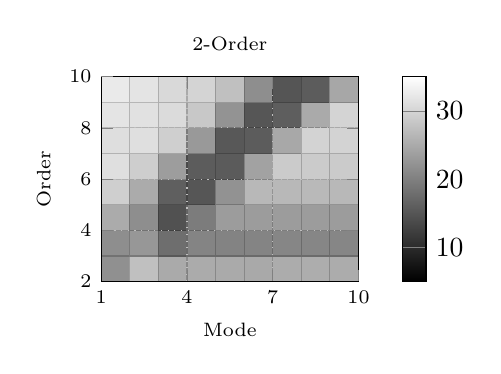
\begin{tikzpicture}
%\begin{axis}[width=0.45\textwidth,style={font=\scriptsize},grid=major,grid style={dotted},align=center,xlabel={Contractionmode},xlabel near ticks,ylabel={Tensorrank},zlabel={Gflops/s},title={2-Order}, xtick={1,4,7,10},xticklabels={1,4,7,10}, ytick={2,4,6,8,10}, yticklabels={2,4,6,8,10}, ztick={5,15,25,35},zticklabels={5,15,25,35}, view={-45}{45}]
%\addplot3[surf,shader=faceted interp, colormap = {whiteblack}{color(0cm)=(white);color(0.4cm) = (darkgray)}] %  colormap/blackwhite
\begin{axis}[width=0.40\textwidth,style={font=\scriptsize},grid=major,grid style={dotted},align=center,xlabel={Mode},ylabel={Order},zlabel={Gflops/s},title={2-Order}, xtick={1,4,7,10},xticklabels={1,4,7,10}, ytick={2,4,6,8,10}, yticklabels={2,4,6,8,10}, point meta max=35, point meta min=5, ztick={5,15,25,35},zticklabels={5,15,25,35}, view={0}{90}, colorbar,colormap/blackwhite, colorbar style={width=0.3cm}]
\addplot3[surf] %  ,colormap/blackwhite ,shader=faceted interp, colormap = {whiteblack}{color(0cm)=(white);color(0.4cm) = (darkgray)}
coordinates{(1.000,2.000,16.487) (1.000,3.000,10.523) (1.000,4.000,15.395) (1.000,5.000,24.073) (1.000,6.000,31.895) (1.000,7.000,30.984) (1.000,8.000,30.758) (1.000,9.000,32.238) (1.000,10.000,32.059) 

(2.000,2.000,30.222) (2.000,3.000,30.212) (2.000,4.000,30.186) (2.000,5.000,30.372) (2.000,6.000,30.553) (2.000,7.000,30.716) (2.000,8.000,31.277) (2.000,9.000,32.485) (2.000,10.000,32.573) 

(3.000,2.000,30.131) (3.000,3.000,19.318) (3.000,4.000,10.731) (3.000,5.000,15.162) (3.000,6.000,23.937) (3.000,7.000,31.261) (3.000,8.000,30.887) (3.000,9.000,30.344) (3.000,10.000,31.150) 

(4.000,2.000,30.361) (4.000,3.000,19.814) (4.000,4.000,21.447) (4.000,5.000,10.324) (4.000,6.000,14.858) (4.000,7.000,23.518) (4.000,8.000,30.873) (4.000,9.000,30.238) (4.000,10.000,29.623) 

(5.000,2.000,30.360) (5.000,3.000,19.462) (5.000,4.000,21.109) (5.000,5.000,25.090) (5.000,6.000,9.819) (5.000,7.000,14.619) (5.000,8.000,22.566) (5.000,9.000,29.901) (5.000,10.000,29.393) 

(6.000,2.000,30.335) (6.000,3.000,19.079) (6.000,4.000,21.407) (6.000,5.000,25.074) (6.000,6.000,28.086) (6.000,7.000,9.972) (6.000,8.000,13.973) (6.000,9.000,22.128) (6.000,10.000,28.208) 

(7.000,2.000,30.310) (7.000,3.000,19.451) (7.000,4.000,21.691) (7.000,5.000,24.793) (7.000,6.000,28.064) (7.000,7.000,29.357) (7.000,8.000,9.892) (7.000,9.000,14.045) (7.000,10.000,21.885) 

(8.000,2.000,30.456) (8.000,3.000,20.016) (8.000,4.000,21.611) (8.000,5.000,24.992) (8.000,6.000,28.120) (8.000,7.000,29.268) (8.000,8.000,30.003) (8.000,9.000,9.867) (8.000,10.000,13.789) 

(9.000,2.000,30.526) (9.000,3.000,19.705) (9.000,4.000,21.412) (9.000,5.000,25.037) (9.000,6.000,28.145) (9.000,7.000,29.169) (9.000,8.000,29.956) (9.000,9.000,29.528) (9.000,10.000,9.665) 

(10.000,2.000,30.524) (10.000,3.000,19.731) (10.000,4.000,21.676) (10.000,5.000,24.930) (10.000,6.000,27.992) (10.000,7.000,29.354) (10.000,8.000,29.951) (10.000,9.000,29.632) (10.000,10.000,29.359) 

};
\end{axis}
\end{tikzpicture}
\end{comment}


%%%%%%%%%%%%%%%%%%%%%%%%%
%%%%%%%%%%%%%%%%%%%%%%%%%

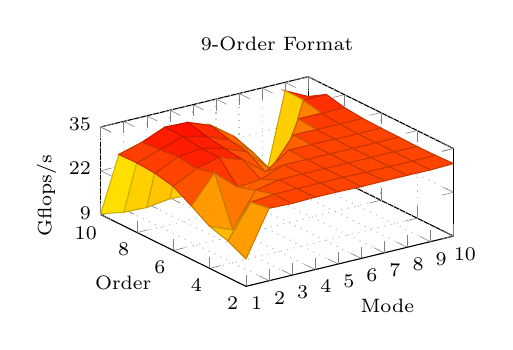
\begin{tikzpicture}
\begin{axis}[height=0.35\textwidth,width=0.5\textwidth,style={font=\scriptsize},grid=major,grid style={dotted},align=center,xlabel={Mode},ylabel={Order},zlabel={Gflops/s},title={$9$-Order Format}, xtick={1,2,3,4,5,6,7,8,9,10},xticklabels={1,2,3,4,5,6,7,8,9,10}, ytick={2,4,6,8,10}, yticklabels={2,4,6,8,10}, point meta max=35, point meta min=9, zmin=9, zmax=35, ztick={9,22,35},zticklabels={9,22,35}, view={-35}{45}, xlabel style={yshift=2mm}, ylabel style={yshift=4mm}, zlabel style={yshift=-1mm,xshift=-4mm}]
\addplot3[surf] %, colormap = {whiteblack}{color(0cm)=(white);color(0.4cm) = (darkgray)}
coordinates{
(1.000,2.000,17.129) (1.000,3.000,19.813) (1.000,4.000,21.480) (1.000,5.000,24.831) (1.000,6.000,28.007) (1.000,7.000,29.212) (1.000,8.000,29.648) (1.000,9.000,29.509) (1.000,10.000,9.204) 

(2.000,2.000,30.515) (2.000,3.000,29.627) (2.000,4.000,18.732) (2.000,5.000,33.044) (2.000,6.000,31.688) (2.000,7.000,32.481) (2.000,8.000,31.983) (2.000,9.000,31.437) (2.000,10.000,8.033) 

(3.000,2.000,30.283) (3.000,3.000,30.326) (3.000,4.000,28.877) (3.000,5.000,27.145) (3.000,6.000,33.324) (3.000,7.000,33.272) (3.000,8.000,34.140) (3.000,9.000,34.297) (3.000,10.000,7.806) 

(4.000,2.000,30.481) (4.000,3.000,30.330) (4.000,4.000,30.260) (4.000,5.000,27.751) (4.000,6.000,31.000) (4.000,7.000,31.675) (4.000,8.000,32.562) (4.000,9.000,34.035) (4.000,10.000,8.720) 

(5.000,2.000,30.460) (5.000,3.000,30.363) (5.000,4.000,30.381) (5.000,5.000,30.380) (5.000,6.000,25.669) (5.000,7.000,28.912) (5.000,8.000,29.837) (5.000,9.000,31.473) (5.000,10.000,8.323) 

(6.000,2.000,30.289) (6.000,3.000,30.392) (6.000,4.000,30.314) (6.000,5.000,30.366) (6.000,6.000,30.487) (6.000,7.000,22.045) (6.000,8.000,24.634) (6.000,9.000,26.550) (6.000,10.000,7.492) 

(7.000,2.000,30.361) (7.000,3.000,30.244) (7.000,4.000,30.325) (7.000,5.000,30.351) (7.000,6.000,30.472) (7.000,7.000,30.667) (7.000,8.000,15.462) (7.000,9.000,17.764) (7.000,10.000,6.490) 

(8.000,2.000,30.368) (8.000,3.000,30.239) (8.000,4.000,30.302) (8.000,5.000,30.322) (8.000,6.000,30.423) (8.000,7.000,30.604) (8.000,8.000,31.118) (8.000,9.000,10.020) (8.000,10.000,3.702) 

(9.000,2.000,30.302) (9.000,3.000,30.263) (9.000,4.000,30.374) (9.000,5.000,30.381) (9.000,6.000,30.290) (9.000,7.000,30.575) (9.000,8.000,31.125) (9.000,9.000,32.377) (9.000,10.000,32.499) 

(10.000,2.000,30.528) (10.000,3.000,30.308) (10.000,4.000,30.248) (10.000,5.000,30.360) (10.000,6.000,30.425) (10.000,7.000,30.623) (10.000,8.000,31.143) (10.000,9.000,32.405) (10.000,10.000,29.128) 

};
\end{axis}
\end{tikzpicture}
\begin{comment}
\begin{tikzpicture}
\begin{axis}[height=0.40\textheight,width=0.40\textwidth,style={font=\footnotesize},grid=major,grid style={dotted},align=center,xlabel={Kontraktionsmodus},ylabel={Tensorstufe},title={TLib-LB-PB1},scaled ticks=false,zticklabel=\pgfmathprintnumber{\tick},zlabel={Durchsatz [Gflops/s]},view={-45}{45}, zlabel={Standardfehler [\%]}]
\addplot3[surf]
coordinates{(1.000,2.000,1.332) (1.000,3.000,2.323) (1.000,4.000,1.343) (1.000,5.000,2.804) (1.000,6.000,2.185) (1.000,7.000,1.776) (1.000,8.000,3.519) (1.000,9.000,1.011) (1.000,10.000,8.378) 

(2.000,2.000,0.982) (2.000,3.000,13.229) (2.000,4.000,9.766) (2.000,5.000,8.786) (2.000,6.000,8.573) (2.000,7.000,7.481) (2.000,8.000,3.903) (2.000,9.000,1.505) (2.000,10.000,10.030) 

(3.000,2.000,3.028) (3.000,3.000,2.194) (3.000,4.000,17.840) (3.000,5.000,17.637) (3.000,6.000,15.227) (3.000,7.000,14.487) (3.000,8.000,8.447) (3.000,9.000,1.892) (3.000,10.000,8.646) 

(4.000,2.000,1.246) (4.000,3.000,2.092) (4.000,4.000,3.240) (4.000,5.000,23.698) (4.000,6.000,23.113) (4.000,7.000,23.313) (4.000,8.000,17.243) (4.000,9.000,7.588) (4.000,10.000,7.767) 

(5.000,2.000,1.784) (5.000,3.000,2.086) (5.000,4.000,2.754) (5.000,5.000,3.265) (5.000,6.000,30.565) (5.000,7.000,31.968) (5.000,8.000,27.869) (5.000,9.000,18.713) (5.000,10.000,9.655) 

(6.000,2.000,3.050) (6.000,3.000,1.930) (6.000,4.000,3.008) (6.000,5.000,3.280) (6.000,6.000,3.699) (6.000,7.000,41.861) (6.000,8.000,40.665) (6.000,9.000,33.483) (6.000,10.000,9.785) 

(7.000,2.000,1.125) (7.000,3.000,2.431) (7.000,4.000,2.940) (7.000,5.000,3.223) (7.000,6.000,3.827) (7.000,7.000,4.337) (7.000,8.000,49.526) (7.000,9.000,47.835) (7.000,10.000,12.546) 

(8.000,2.000,1.147) (8.000,3.000,2.508) (8.000,4.000,3.005) (8.000,5.000,2.770) (8.000,6.000,3.539) (8.000,7.000,3.996) (8.000,8.000,4.144) (8.000,9.000,58.162) (8.000,10.000,13.963) 

(9.000,2.000,3.252) (9.000,3.000,2.411) (9.000,4.000,2.776) (9.000,5.000,3.117) (9.000,6.000,5.433) (9.000,7.000,4.170) (9.000,8.000,4.123) (9.000,9.000,0.672) (9.000,10.000,0.797) 

(10.000,2.000,1.467) (10.000,3.000,2.076) (10.000,4.000,3.202) (10.000,5.000,3.244) (10.000,6.000,3.931) (10.000,7.000,4.243) (10.000,8.000,4.159) (10.000,9.000,1.011) (10.000,10.000,2.226) 

};\end{axis}
\end{tikzpicture}
\end{comment}
\begin{comment}
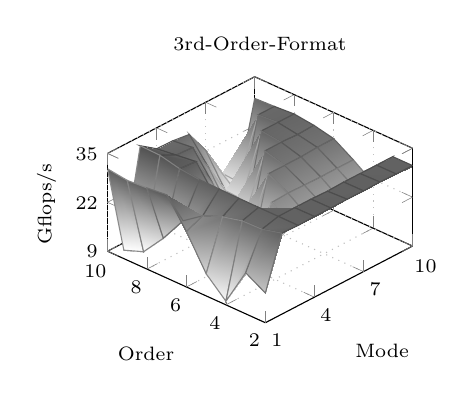
\begin{tikzpicture}
\begin{axis}[width=0.45\textwidth,style={font=\scriptsize},grid=major,grid style={dotted},align=center,xlabel={Mode},ylabel={Order},zlabel={Gflops/s},title={3rd-Order-Format}, xtick={1,4,7,10},xticklabels={1,4,7,10}, ytick={2,4,6,8,10}, yticklabels={2,4,6,8,10}, point meta max=35, point meta min=9, zmin=9, zmax=35, ztick={9,22,35},zticklabels={9,22,35}, view={-47}{47}, ] %
\addplot3[surf,shader=faceted interp, colormap = {whiteblack}{color(0cm)=(white);color(0.4cm) = (darkgray)}] %  colormap/blackwhite
coordinates{
(1.000,2.000,16.903) (1.000,3.000,19.899) (1.000,4.000,9.972) (1.000,5.000,14.884) (1.000,6.000,23.730) (1.000,7.000,31.140) (1.000,8.000,30.576) (1.000,9.000,30.207) (1.000,10.000,30.915) 

(2.000,2.000,30.562) (2.000,3.000,29.215) (2.000,4.000,29.073) (2.000,5.000,27.765) (2.000,6.000,25.665) (2.000,7.000,21.957) (2.000,8.000,14.935) (2.000,9.000,8.976) (2.000,10.000,7.009) 

(3.000,2.000,30.335) (3.000,3.000,30.356) (3.000,4.000,30.356) (3.000,5.000,30.404) (3.000,6.000,30.503) (3.000,7.000,30.627) (3.000,8.000,31.162) (3.000,9.000,32.369) (3.000,10.000,32.511) 

(4.000,2.000,30.443) (4.000,3.000,30.413) (4.000,4.000,21.309) (4.000,5.000,10.070) (4.000,6.000,14.819) (4.000,7.000,23.495) (4.000,8.000,30.785) (4.000,9.000,30.121) (4.000,10.000,29.447) 

(5.000,2.000,30.441) (5.000,3.000,30.415) (5.000,4.000,21.189) (5.000,5.000,24.741) (5.000,6.000,9.830) (5.000,7.000,14.105) (5.000,8.000,22.859) (5.000,9.000,29.890) (5.000,10.000,29.293) 

(6.000,2.000,30.501) (6.000,3.000,30.264) (6.000,4.000,21.327) (6.000,5.000,24.995) (6.000,6.000,27.759) (6.000,7.000,9.373) (6.000,8.000,13.735) (6.000,9.000,22.080) (6.000,10.000,28.726) 

(7.000,2.000,30.463) (7.000,3.000,30.424) (7.000,4.000,21.552) (7.000,5.000,24.845) (7.000,6.000,27.708) (7.000,7.000,29.197) (7.000,8.000,9.455) (7.000,9.000,13.912) (7.000,10.000,22.226) 

(8.000,2.000,30.559) (8.000,3.000,30.409) (8.000,4.000,21.183) (8.000,5.000,24.771) (8.000,6.000,27.728) (8.000,7.000,29.236) (8.000,8.000,29.881) (8.000,9.000,9.399) (8.000,10.000,13.882) 

(9.000,2.000,30.413) (9.000,3.000,30.383) (9.000,4.000,21.371) (9.000,5.000,24.801) (9.000,6.000,27.975) (9.000,7.000,29.032) (9.000,8.000,29.869) (9.000,9.000,29.502) (9.000,10.000,9.277) 

(10.000,2.000,30.391) (10.000,3.000,30.378) (10.000,4.000,21.091) (10.000,5.000,24.776) (10.000,6.000,28.059) (10.000,7.000,29.208) (10.000,8.000,29.848) (10.000,9.000,29.484) (10.000,10.000,29.241) 

};
\end{axis}
\end{tikzpicture}
\end{comment}
\begin{comment}
\begin{tikzpicture}
\begin{axis}[height=0.40\textheight,width=0.40\textwidth,style={font=\footnotesize},grid=major,grid style={dotted},align=center,xlabel={Kontraktionsmodus},ylabel={Tensorstufe},title={TLib-LB-PB2},scaled ticks=false,zticklabel=\pgfmathprintnumber{\tick},zlabel={Durchsatz [Gflops/s]},view={-45}{45}, zlabel={Standardfehler [\%]}]
\addplot3[surf]
coordinates{(1.000,2.000,1.307) (1.000,3.000,1.302) (1.000,4.000,10.940) (1.000,5.000,4.791) (1.000,6.000,2.662) (1.000,7.000,1.372) (1.000,8.000,1.192) (1.000,9.000,1.793) (1.000,10.000,1.223) 

(2.000,2.000,1.359) (2.000,3.000,14.470) (2.000,4.000,18.614) (2.000,5.000,23.954) (2.000,6.000,30.664) (2.000,7.000,42.176) (2.000,8.000,49.976) (2.000,9.000,48.495) (2.000,10.000,72.280) 

(3.000,2.000,1.730) (3.000,3.000,2.233) (3.000,4.000,2.992) (3.000,5.000,3.202) (3.000,6.000,3.692) (3.000,7.000,4.356) (3.000,8.000,4.346) (3.000,9.000,1.336) (3.000,10.000,0.967) 

(4.000,2.000,1.249) (4.000,3.000,2.217) (4.000,4.000,1.868) (4.000,5.000,10.989) (4.000,6.000,5.915) (4.000,7.000,1.652) (4.000,8.000,1.266) (4.000,9.000,1.297) (4.000,10.000,1.679) 

(5.000,2.000,1.654) (5.000,3.000,2.156) (5.000,4.000,2.024) (5.000,5.000,2.917) (5.000,6.000,9.904) (5.000,7.000,6.006) (5.000,8.000,2.559) (5.000,9.000,0.933) (5.000,10.000,1.096) 

(6.000,2.000,1.519) (6.000,3.000,2.374) (6.000,4.000,1.717) (6.000,5.000,2.551) (6.000,6.000,2.491) (6.000,7.000,11.882) (6.000,8.000,6.486) (6.000,9.000,2.339) (6.000,10.000,2.331) 

(7.000,2.000,1.545) (7.000,3.000,2.096) (7.000,4.000,1.423) (7.000,5.000,2.617) (7.000,6.000,2.637) (7.000,7.000,1.911) (7.000,8.000,11.610) (7.000,9.000,5.473) (7.000,10.000,2.849) 

(8.000,2.000,1.677) (8.000,3.000,2.111) (8.000,4.000,1.871) (8.000,5.000,2.775) (8.000,6.000,2.158) (8.000,7.000,1.943) (8.000,8.000,1.400) (8.000,9.000,10.778) (8.000,10.000,5.460) 

(9.000,2.000,1.534) (9.000,3.000,2.010) (9.000,4.000,1.628) (9.000,5.000,2.494) (9.000,6.000,2.310) (9.000,7.000,2.047) (9.000,8.000,1.370) (9.000,9.000,1.302) (9.000,10.000,10.568) 

(10.000,2.000,1.603) (10.000,3.000,2.075) (10.000,4.000,1.484) (10.000,5.000,2.817) (10.000,6.000,2.233) (10.000,7.000,1.943) (10.000,8.000,1.591) (10.000,9.000,1.081) (10.000,10.000,0.938) 

};\end{axis}
\end{tikzpicture}
\end{comment}
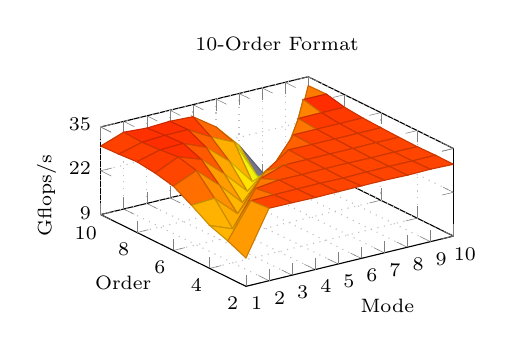
\begin{tikzpicture}
\begin{axis}[height=0.35\textwidth, width=0.5\textwidth,,style={font=\scriptsize},grid=major,grid style={dotted}, align=center, xlabel={Mode}, ylabel={Order}, zlabel={Gflops/s},title={$10$-Order Format}, xtick={1,4,7,10}, xtick={1,2,3,4,5,6,7,8,9,10},xticklabels={1,2,3,4,5,6,7,8,9,10}, ytick={2,4,6,8,10}, yticklabels={2,4,6,8,10}, point meta max=35, point meta min=9, zmin=9, zmax=35, ztick={9,22,35},zticklabels={9,22,35}, view={-35}{45}, xlabel style={yshift=2mm}, ylabel style={yshift=4mm}, zlabel style={yshift=-1mm,xshift=-4mm}]
\addplot3[surf] %, colormap = {whiteblack}{color(0cm)=(white);color(0.4cm) = (darkgray)}
coordinates{
(1.000,2.000,17.409) (1.000,3.000,19.812) (1.000,4.000,21.745) (1.000,5.000,25.078) (1.000,6.000,28.085) (1.000,7.000,29.298) (1.000,8.000,29.987) (1.000,9.000,29.593) (1.000,10.000,29.331) 

(2.000,2.000,30.526) (2.000,3.000,30.078) (2.000,4.000,19.075) (2.000,5.000,25.485) (2.000,6.000,31.053) (2.000,7.000,32.425) (2.000,8.000,31.856) (2.000,9.000,31.451) (2.000,10.000,31.793) 

(3.000,2.000,30.491) (3.000,3.000,30.201) (3.000,4.000,29.403) (3.000,5.000,19.233) (3.000,6.000,25.043) (3.000,7.000,30.057) (3.000,8.000,32.131) (3.000,9.000,31.868) (3.000,10.000,31.353) 

(4.000,2.000,30.377) (4.000,3.000,30.243) (4.000,4.000,30.257) (4.000,5.000,28.016) (4.000,6.000,18.205) (4.000,7.000,24.081) (4.000,8.000,29.305) (4.000,9.000,31.878) (4.000,10.000,31.729) 

(5.000,2.000,30.460) (5.000,3.000,30.290) (5.000,4.000,30.209) (5.000,5.000,30.359) (5.000,6.000,25.869) (5.000,7.000,17.267) (5.000,8.000,23.559) (5.000,9.000,28.071) (5.000,10.000,31.424) 

(6.000,2.000,30.511) (6.000,3.000,30.166) (6.000,4.000,30.321) (6.000,5.000,30.355) (6.000,6.000,30.564) (6.000,7.000,21.926) (6.000,8.000,15.802) (6.000,9.000,24.870) (6.000,10.000,26.742) 

(7.000,2.000,30.538) (7.000,3.000,30.319) (7.000,4.000,30.306) (7.000,5.000,30.361) (7.000,6.000,30.511) (7.000,7.000,30.708) (7.000,8.000,14.834) (7.000,9.000,13.136) (7.000,10.000,19.648) 

(8.000,2.000,30.384) (8.000,3.000,30.339) (8.000,4.000,30.214) (8.000,5.000,30.330) (8.000,6.000,30.492) (8.000,7.000,30.739) (8.000,8.000,31.234) (8.000,9.000,8.582) (8.000,10.000,10.020) 

(9.000,2.000,30.498) (9.000,3.000,30.302) (9.000,4.000,30.260) (9.000,5.000,30.396) (9.000,6.000,30.486) (9.000,7.000,30.730) (9.000,8.000,31.287) (9.000,9.000,32.548) (9.000,10.000,6.632) 

(10.000,2.000,30.308) (10.000,3.000,30.366) (10.000,4.000,30.223) (10.000,5.000,30.347) (10.000,6.000,30.530) (10.000,7.000,30.767) (10.000,8.000,31.274) (10.000,9.000,32.506) (10.000,10.000,32.361) 

};
\end{axis}
\end{tikzpicture}
\begin{comment}
\begin{tikzpicture}
\begin{axis}[height=0.40\textheight,width=0.40\textwidth,style={font=\footnotesize},grid=major,grid style={dotted},align=center,xlabel={Kontraktionsmodus},ylabel={Tensorstufe},title={TLib-LB-PB2},scaled ticks=false,zticklabel=\pgfmathprintnumber{\tick},zlabel={Durchsatz [Gflops/s]},view={-45}{45}, zlabel={Standardfehler [\%]}]
\addplot3[surf]
coordinates{(1.000,2.000,4.564) (1.000,3.000,0.857) (1.000,4.000,1.351) (1.000,5.000,2.682) (1.000,6.000,2.343) (1.000,7.000,1.887) (1.000,8.000,1.623) (1.000,9.000,1.073) (1.000,10.000,0.554) 

(2.000,2.000,1.631) (2.000,3.000,14.436) (2.000,4.000,9.826) (2.000,5.000,9.686) (2.000,6.000,8.965) (2.000,7.000,6.260) (2.000,8.000,3.487) (2.000,9.000,1.181) (2.000,10.000,0.824) 

(3.000,2.000,1.700) (3.000,3.000,2.889) (3.000,4.000,17.852) (3.000,5.000,13.035) (3.000,6.000,14.371) (3.000,7.000,16.050) (3.000,8.000,8.848) (3.000,9.000,3.169) (3.000,10.000,1.302) 

(4.000,2.000,1.970) (4.000,3.000,2.697) (4.000,4.000,3.434) (4.000,5.000,24.038) (4.000,6.000,18.289) (4.000,7.000,19.803) (4.000,8.000,16.449) (4.000,9.000,7.402) (4.000,10.000,2.932) 

(5.000,2.000,1.644) (5.000,3.000,2.583) (5.000,4.000,3.771) (5.000,5.000,3.849) (5.000,6.000,30.722) (5.000,7.000,23.552) (5.000,8.000,22.359) (5.000,9.000,17.913) (5.000,10.000,8.220) 

(6.000,2.000,1.755) (6.000,3.000,3.028) (6.000,4.000,3.140) (6.000,5.000,3.226) (6.000,6.000,3.913) (6.000,7.000,42.319) (6.000,8.000,29.211) (6.000,9.000,32.995) (6.000,10.000,21.344) 

(7.000,2.000,1.635) (7.000,3.000,2.569) (7.000,4.000,3.437) (7.000,5.000,3.747) (7.000,6.000,4.086) (7.000,7.000,4.594) (7.000,8.000,50.529) (7.000,9.000,34.822) (7.000,10.000,37.357) 

(8.000,2.000,1.316) (8.000,3.000,2.385) (8.000,4.000,3.803) (8.000,5.000,3.873) (8.000,6.000,4.225) (8.000,7.000,4.245) (8.000,8.000,4.301) (8.000,9.000,44.414) (8.000,10.000,37.792) 

(9.000,2.000,1.683) (9.000,3.000,2.600) (9.000,4.000,3.460) (9.000,5.000,3.429) (9.000,6.000,4.282) (9.000,7.000,4.528) (9.000,8.000,4.303) (9.000,9.000,1.485) (9.000,10.000,70.528) 

(10.000,2.000,2.128) (10.000,3.000,2.423) (10.000,4.000,3.819) (10.000,5.000,3.950) (10.000,6.000,4.060) (10.000,7.000,4.532) (10.000,8.000,4.209) (10.000,9.000,1.213) (10.000,10.000,4.486) 

};
\end{axis}
\end{tikzpicture}
\end{comment}

	\caption{
		\footnotesize Average performance maps of the \tf{TLIB-LB-PN} implementation with varying contraction modes and tensor order. 
		Tensor elements are encoded in single-precision and stored contiguously in memory according to the $1$-order, $2$-order, $9$-order and $10$-order storage format, respectively. 
		Tensors are \tit{asymmetrically}-\tit{shaped} with dimensions from the first test setup.
		%Arithmetic mean is calculated over the tensor size.
		\label{fig:performance.tlib.lb.layout.single.surf.nonsymmetric}
	}
\end{figure*}
\end{comment}
\begin{figure*}[t]
	\begin{tikzpicture}
\begin{axis}[height=0.2\textheight,width=0.35\textwidth,style={font=\scriptsize},grid=major,grid style={dotted},align=center,xlabel={Mode},ylabel={Order},title={\ttt{TCL}}, scaled ticks=false, xtick={2,4,6,8,10}, xticklabels={2,4,6,8,10}, ytick={2,4,6,8,10}, yticklabels={2,4,6,8,10}, point meta max=23, point meta min=1, zmin=1, zmax=23, ztick={1,12,23},zticklabels={1,12,23}, zlabel={Gflops/s}, view={-35}{45}, xlabel style={yshift=2mm}, ylabel style={yshift=5mm}, zlabel style={yshift=-1mm,xshift=-4mm}, title style={yshift=-2mm}] % ,
\addplot3[surf] %, colormap = {whiteblack}{color(0cm)=(white);color(0.4cm) = (darkgray)}
coordinates{
(1.000,2.000,22.456) (1.000,3.000,22.094) (1.000,4.000,7.206) (1.000,5.000,7.143) (1.000,6.000,7.285) (1.000,7.000,7.364) (1.000,8.000,7.105) (1.000,9.000,7.222) (1.000,10.000,7.174) 

(2.000,2.000,1.936) (2.000,3.000,1.808) (2.000,4.000,0.727) (2.000,5.000,0.859) (2.000,6.000,1.099) (2.000,7.000,1.588) (2.000,8.000,2.220) (2.000,9.000,2.761) (2.000,10.000,3.681) 

(3.000,2.000,1.920) (3.000,3.000,1.766) (3.000,4.000,0.652) (3.000,5.000,0.755) (3.000,6.000,0.848) (3.000,7.000,1.063) (3.000,8.000,1.485) (3.000,9.000,2.138) (3.000,10.000,2.658) 

(4.000,2.000,1.938) (4.000,3.000,1.745) (4.000,4.000,0.610) (4.000,5.000,0.721) (4.000,6.000,0.783) (4.000,7.000,0.899) (4.000,8.000,1.093) (4.000,9.000,1.501) (4.000,10.000,2.181) 

(6.000,2.000,1.931) (6.000,3.000,1.759) (6.000,4.000,0.613) (6.000,5.000,0.695) (6.000,6.000,0.761) (6.000,7.000,0.867) (6.000,8.000,1.026) (6.000,9.000,1.183) (6.000,10.000,1.628) 

(7.000,2.000,1.913) (7.000,3.000,1.782) (7.000,4.000,0.609) (7.000,5.000,0.701) (7.000,6.000,0.760) (7.000,7.000,0.922) (7.000,8.000,1.072) (7.000,9.000,1.196) (7.000,10.000,1.623) 

(8.000,2.000,1.916) (8.000,3.000,1.758) (8.000,4.000,0.612) (8.000,5.000,0.699) (8.000,6.000,0.765) (8.000,7.000,0.933) (8.000,8.000,1.161) (8.000,9.000,1.270) (8.000,10.000,1.650) 

(9.000,2.000,1.894) (9.000,3.000,1.770) (9.000,4.000,0.608) (9.000,5.000,0.702) (9.000,6.000,0.763) (9.000,7.000,0.922) (9.000,8.000,1.167) (9.000,9.000,1.464) (9.000,10.000,1.687) 

(10.000,2.000,1.915) (10.000,3.000,1.761) (10.000,4.000,0.615) (10.000,5.000,0.705) (10.000,6.000,0.763) (10.000,7.000,0.919) (10.000,8.000,1.149) (10.000,9.000,1.452) (10.000,10.000,2.038) 

};
\end{axis}
\end{tikzpicture}
\begin{comment}
\begin{tikzpicture}
\begin{axis}[height=0.25\textheight,width=0.3\textwidth,style={font=\scriptsize},grid=major,grid style={dotted},align=center,xlabel={Mode},ylabel={Order},title={TCL},scaled ticks=false,zticklabel=\pgfmathprintnumber{\tick},zlabel={Gflops/s},view={-45}{45}, zlabel={Standardfehler [\%]}]
\addplot3[surf]
coordinates{
(1.000,2.000,22.642) (1.000,3.000,15.424) (1.000,4.000,6.600) (1.000,5.000,9.366) (1.000,6.000,6.103) (1.000,7.000,6.326) (1.000,8.000,9.184) (1.000,9.000,6.843) (1.000,10.000,10.211) 

(2.000,2.000,14.252) (2.000,3.000,19.264) (2.000,4.000,37.164) (2.000,5.000,40.227) (2.000,6.000,51.492) (2.000,7.000,47.107) (2.000,8.000,39.097) (2.000,9.000,38.480) (2.000,10.000,33.946) 

(3.000,2.000,13.449) (3.000,3.000,13.211) (3.000,4.000,19.551) (3.000,5.000,33.191) (3.000,6.000,41.243) (3.000,7.000,50.661) (3.000,8.000,50.632) (3.000,9.000,35.379) (3.000,10.000,32.449) 

(4.000,2.000,15.721) (4.000,3.000,15.754) (4.000,4.000,23.373) (4.000,5.000,32.804) (4.000,6.000,35.998) (4.000,7.000,55.167) (4.000,8.000,57.355) (4.000,9.000,56.130) (4.000,10.000,37.866) 

(6.000,2.000,8.194) (6.000,3.000,16.002) (6.000,4.000,22.827) (6.000,5.000,36.494) (6.000,6.000,44.103) (6.000,7.000,54.573) (6.000,8.000,67.934) (6.000,9.000,65.625) (6.000,10.000,62.020) 

(7.000,2.000,10.694) (7.000,3.000,15.072) (7.000,4.000,21.784) (7.000,5.000,37.209) (7.000,6.000,41.483) (7.000,7.000,53.899) (7.000,8.000,64.716) (7.000,9.000,68.793) (7.000,10.000,62.875) 

(8.000,2.000,14.520) (8.000,3.000,16.172) (8.000,4.000,22.225) (8.000,5.000,34.791) (8.000,6.000,42.029) (8.000,7.000,56.385) (8.000,8.000,70.738) (8.000,9.000,73.910) (8.000,10.000,65.133) 

(9.000,2.000,14.687) (9.000,3.000,15.408) (9.000,4.000,22.700) (9.000,5.000,36.494) (9.000,6.000,43.393) (9.000,7.000,54.136) (9.000,8.000,70.710) (9.000,9.000,67.720) (9.000,10.000,63.282) 

(10.000,2.000,14.496) (10.000,3.000,16.808) (10.000,4.000,23.509) (10.000,5.000,36.675) (10.000,6.000,41.853) (10.000,7.000,53.597) (10.000,8.000,66.302) (10.000,9.000,66.482) (10.000,10.000,51.423) 

};
\end{axis}
\end{tikzpicture}
\end{comment}
\hfill
\begin{tikzpicture}
\begin{axis}[height=0.2\textheight,width=0.35\textwidth,style={font=\scriptsize},grid=major,grid style={dotted},align=center,xlabel={Mode},ylabel={Order},title={\ttt{TBLIS}}, scaled ticks=false, xtick={2,4,6,8,10}, xticklabels={2,4,6,8,10}, ytick={2,4,6,8,10}, yticklabels={2,4,6,8,10},  point meta max=11, point meta min=5, zmin=5, zmax=11, ztick={5,8,11},zticklabels={5,8,11}, zlabel={Gflops/s},view={-35}{45}, xlabel style={yshift=2mm}, ylabel style={yshift=5mm}, zlabel style={yshift=-1mm,xshift=-4mm}, title style={yshift=-2mm}]
\addplot3[surf] %, colormap = {whiteblack}{color(0cm)=(white);color(0.4cm) = (darkgray)}
coordinates{
(1.000,2.000,8.056) (1.000,3.000,8.924) (1.000,4.000,9.473) (1.000,5.000,9.750) (1.000,6.000,9.251) (1.000,7.000,9.771) (1.000,8.000,10.006) (1.000,9.000,10.304) (1.000,10.000,9.868) 

(2.000,2.000,6.594) (2.000,3.000,8.123) (2.000,4.000,9.431) (2.000,5.000,9.824) (2.000,6.000,9.122) (2.000,7.000,9.130) (2.000,8.000,9.093) (2.000,9.000,9.135) (2.000,10.000,9.214) 

(3.000,2.000,6.716) (3.000,3.000,5.978) (3.000,4.000,7.856) (3.000,5.000,8.009) (3.000,6.000,7.851) (3.000,7.000,7.794) (3.000,8.000,7.757) (3.000,9.000,7.965) (3.000,10.000,7.945) 

(4.000,2.000,6.619) (4.000,3.000,5.990) (4.000,4.000,7.486) (4.000,5.000,7.580) (4.000,6.000,7.260) (4.000,7.000,7.214) (4.000,8.000,7.220) (4.000,9.000,6.743) (4.000,10.000,7.004) 

(6.000,2.000,6.723) (6.000,3.000,5.868) (6.000,4.000,6.619) (6.000,5.000,6.046) (6.000,6.000,5.970) (6.000,7.000,5.710) (6.000,8.000,5.891) (6.000,9.000,5.823) (6.000,10.000,5.773) 

(7.000,2.000,6.735) (7.000,3.000,5.918) (7.000,4.000,6.923) (7.000,5.000,5.793) (7.000,6.000,6.162) (7.000,7.000,6.069) (7.000,8.000,5.798) (7.000,9.000,5.440) (7.000,10.000,5.408) 

(8.000,2.000,6.712) (8.000,3.000,5.919) (8.000,4.000,6.637) (8.000,5.000,5.662) (8.000,6.000,6.187) (8.000,7.000,5.632) (8.000,8.000,5.838) (8.000,9.000,5.908) (8.000,10.000,5.531) 

(9.000,2.000,6.679) (9.000,3.000,6.169) (9.000,4.000,6.940) (9.000,5.000,5.858) (9.000,6.000,6.013) (9.000,7.000,6.044) (9.000,8.000,5.925) (9.000,9.000,5.838) (9.000,10.000,5.535) 

(10.000,2.000,6.510) (10.000,3.000,5.818) (10.000,4.000,6.465) (10.000,5.000,5.631) (10.000,6.000,5.905) (10.000,7.000,5.480) (10.000,8.000,5.960) (10.000,9.000,5.935) (10.000,10.000,5.795) 


};
\end{axis}
\end{tikzpicture}
\begin{comment}
\begin{tikzpicture}
\begin{axis}[height=0.25\textheight,width=0.3\textwidth,style={font=\scriptsize},grid=major,grid style={dotted},align=center,xlabel={Mode},ylabel={Order},title={TBLIS},scaled ticks=false,zticklabel=\pgfmathprintnumber{\tick},zlabel={Gflops/s},view={-45}{45}, zlabel={Standardfehler [\%]}]
\addplot3[surf]
coordinates{
(1.000,2.000,14.730) (1.000,3.000,8.524) (1.000,4.000,11.426) (1.000,5.000,10.155) (1.000,6.000,6.509) (1.000,7.000,8.492) (1.000,8.000,9.587) (1.000,9.000,10.999) (1.000,10.000,11.072) 

(2.000,2.000,5.945) (2.000,3.000,5.711) (2.000,4.000,6.823) (2.000,5.000,7.575) (2.000,6.000,7.714) (2.000,7.000,8.068) (2.000,8.000,7.474) (2.000,9.000,6.964) (2.000,10.000,7.310) 

(3.000,2.000,5.117) (3.000,3.000,5.224) (3.000,4.000,7.150) (3.000,5.000,6.026) (3.000,6.000,6.899) (3.000,7.000,6.805) (3.000,8.000,7.133) (3.000,9.000,5.931) (3.000,10.000,5.978) 

(4.000,2.000,7.250) (4.000,3.000,5.954) (4.000,4.000,7.465) (4.000,5.000,5.717) (4.000,6.000,3.978) (4.000,7.000,6.547) (4.000,8.000,6.094) (4.000,9.000,13.217) (4.000,10.000,5.921) 

(6.000,2.000,4.515) (6.000,3.000,7.737) (6.000,4.000,6.650) (6.000,5.000,6.805) (6.000,6.000,9.231) (6.000,7.000,13.050) (6.000,8.000,5.949) (6.000,9.000,7.607) (6.000,10.000,9.342) 

(7.000,2.000,3.625) (7.000,3.000,5.911) (7.000,4.000,11.458) (7.000,5.000,12.697) (7.000,6.000,3.434) (7.000,7.000,8.786) (7.000,8.000,6.701) (7.000,9.000,15.042) (7.000,10.000,15.952) 

(8.000,2.000,3.804) (8.000,3.000,2.719) (8.000,4.000,8.299) (8.000,5.000,15.371) (8.000,6.000,2.821) (8.000,7.000,15.637) (8.000,8.000,11.543) (8.000,9.000,6.900) (8.000,10.000,15.249) 

(9.000,2.000,6.272) (9.000,3.000,1.206) (9.000,4.000,5.460) (9.000,5.000,9.223) (9.000,6.000,9.533) (9.000,7.000,4.104) (9.000,8.000,12.228) (9.000,9.000,10.853) (9.000,10.000,16.099) 

(10.000,2.000,9.075) (10.000,3.000,5.961) (10.000,4.000,9.959) (10.000,5.000,15.030) (10.000,6.000,7.924) (10.000,7.000,16.783) (10.000,8.000,10.619) (10.000,9.000,12.958) (10.000,10.000,10.422) 

};
\end{axis}
\end{tikzpicture}
\end{comment}
%\caption{
%\footnotesize Dargestellt sind über die Tensorgröße gemittelten \textbf{Durchsätze in Gflops} der \textbf{Tensor}"=\textbf{Vektor}"=\textbf{Multiplikation}.  Daten sind in \textbf{Floating-Point<Single>} codiert.
%\label{fig:ttv_surf_perf_float}
%}
%\end{figure}
%\clearpage
%\begin{figure}[H]
%\centering
\hfill
\begin{tikzpicture}
\begin{axis}[height=0.2\textheight,width=0.35\textwidth,style={font=\scriptsize},grid=major,grid style={dotted},align=center,xlabel={Mode},ylabel={Order},title={\ttt{EIGEN}}, scaled ticks=false, xtick={2,4,6,8,10}, xticklabels={2,4,6,8,10}, ytick={2,4,6,8,10}, yticklabels={2,4,6,8,10}, point meta max=8, point meta min=2, zmin=2, zmax=8, ztick={2,5,8},zticklabels={2,5,8}, zlabel={Gflops/s},view={-35}{45}, xlabel style={yshift=2mm}, ylabel style={yshift=5mm}, zlabel style={yshift=-1mm,xshift=-4mm}, title style={yshift=-2mm}]
\addplot3[surf] %, colormap = {whiteblack}{color(0cm)=(white);color(0.4cm) = (darkgray)}
coordinates{
%(1.000,2.000,0.614) (1.000,3.000,0.197) (1.000,4.000,0.108) (1.000,5.000,0.086) (1.000,6.000,0.072) (1.000,7.000,0.064) (1.000,8.000,0.056) (1.000,9.000,0.049) (1.000,10.000,0.044) 

(2.000,2.000,7.175) (2.000,3.000,5.427) (2.000,4.000,4.655) (2.000,5.000,4.198) (2.000,6.000,3.577) (2.000,7.000,3.163) (2.000,8.000,2.840) (2.000,9.000,2.556) (2.000,10.000,2.321) 

(3.000,2.000,7.180) (3.000,3.000,6.205) (3.000,4.000,4.718) (3.000,5.000,4.195) (3.000,6.000,3.626) (3.000,7.000,3.193) (3.000,8.000,2.860) (3.000,9.000,2.593) (3.000,10.000,2.328) 

(4.000,2.000,7.204) (4.000,3.000,6.344) (4.000,4.000,5.725) (4.000,5.000,4.136) (4.000,6.000,3.579) (4.000,7.000,3.175) (4.000,8.000,2.827) (4.000,9.000,2.560) (4.000,10.000,2.320) 

(6.000,2.000,7.194) (6.000,3.000,6.332) (6.000,4.000,5.809) (6.000,5.000,3.588) (6.000,6.000,2.866) (6.000,7.000,3.059) (6.000,8.000,2.769) (6.000,9.000,2.533) (6.000,10.000,2.280) 

(7.000,2.000,7.193) (7.000,3.000,6.338) (7.000,4.000,5.711) (7.000,5.000,3.563) (7.000,6.000,2.875) (7.000,7.000,2.311) (7.000,8.000,2.787) (7.000,9.000,2.515) (7.000,10.000,2.280) 

(8.000,2.000,7.216) (8.000,3.000,6.273) (8.000,4.000,5.758) (8.000,5.000,3.539) (8.000,6.000,2.878) (8.000,7.000,2.338) (8.000,8.000,2.016) (8.000,9.000,2.512) (8.000,10.000,2.293) 

(9.000,2.000,7.078) (9.000,3.000,6.337) (9.000,4.000,5.779) (9.000,5.000,3.574) (9.000,6.000,2.886) (9.000,7.000,2.301) (9.000,8.000,2.006) (9.000,9.000,1.735) (9.000,10.000,2.286) 

(10.000,2.000,7.279) (10.000,3.000,6.215) (10.000,4.000,5.712) (10.000,5.000,3.591) (10.000,6.000,2.898) (10.000,7.000,2.313) (10.000,8.000,1.986) (10.000,9.000,1.728) (10.000,10.000,1.593) 

};
\end{axis}
\end{tikzpicture}
\begin{comment}
\begin{tikzpicture}
\begin{axis}[height=0.25\textheight,width=0.3\textwidth,style={font=\scriptsize},grid=major,grid style={dotted},align=center,xlabel={Mode},ylabel={Order},title={EIGEN},scaled ticks=false,zticklabel=\pgfmathprintnumber{\tick},zlabel={Gflops/s},view={-45}{45}, zlabel={Standardfehler [\%]}]
\addplot3[surf]
coordinates{(1.000,2.000,21.045) (1.000,3.000,8.941) (1.000,4.000,7.637) (1.000,5.000,8.191) (1.000,6.000,11.831) (1.000,7.000,10.046) (1.000,8.000,7.536) (1.000,9.000,5.436) (1.000,10.000,2.240) 

(2.000,2.000,1.213) (2.000,3.000,1.924) (2.000,4.000,1.875) (2.000,5.000,0.647) (2.000,6.000,0.626) (2.000,7.000,1.061) (2.000,8.000,1.457) (2.000,9.000,1.710) (2.000,10.000,2.184) 

(3.000,2.000,0.878) (3.000,3.000,0.879) (3.000,4.000,1.410) (3.000,5.000,0.851) (3.000,6.000,1.161) (3.000,7.000,0.767) (3.000,8.000,0.961) (3.000,9.000,1.372) (3.000,10.000,2.241) 

(4.000,2.000,1.929) (4.000,3.000,1.146) (4.000,4.000,1.294) (4.000,5.000,1.482) (4.000,6.000,0.765) (4.000,7.000,0.899) (4.000,8.000,0.972) (4.000,9.000,0.854) (4.000,10.000,1.347) 

(6.000,2.000,1.720) (6.000,3.000,1.466) (6.000,4.000,2.151) (6.000,5.000,1.361) (6.000,6.000,1.122) (6.000,7.000,2.041) (6.000,8.000,1.296) (6.000,9.000,1.556) (6.000,10.000,1.812) 

(7.000,2.000,0.925) (7.000,3.000,0.944) (7.000,4.000,1.543) (7.000,5.000,1.445) (7.000,6.000,0.789) (7.000,7.000,1.095) (7.000,8.000,1.196) (7.000,9.000,1.898) (7.000,10.000,2.490) 

(8.000,2.000,0.896) (8.000,3.000,1.725) (8.000,4.000,1.662) (8.000,5.000,0.850) (8.000,6.000,1.125) (8.000,7.000,0.669) (8.000,8.000,0.951) (8.000,9.000,1.220) (8.000,10.000,2.128) 

(9.000,2.000,1.074) (9.000,3.000,1.326) (9.000,4.000,1.561) (9.000,5.000,0.988) (9.000,6.000,1.093) (9.000,7.000,0.579) (9.000,8.000,1.268) (9.000,9.000,0.749) (9.000,10.000,1.605) 

(10.000,2.000,1.100) (10.000,3.000,1.411) (10.000,4.000,1.012) (10.000,5.000,0.820) (10.000,6.000,0.869) (10.000,7.000,0.777) (10.000,8.000,0.849) (10.000,9.000,0.781) (10.000,10.000,19.561) 

};
\end{axis}
\end{tikzpicture}
\end{comment}
%\caption{
%\footnotesize Dargestellt sind über die Tensorgröße gemittelten \textbf{Durchsätze in Gflops} der \textbf{Tensor}"=\textbf{Vektor}"=\textbf{Multiplikation}.  Daten sind in \textbf{Floating-Point<Single>} codiert.
%\label{fig:ttv_surf_perf_float}
%}
%\end{figure}

	
	\begin{comment}
\begin{tikzpicture}
\begin{axis}[height=0.40\textheight,width=0.40\textwidth,style={font=\footnotesize},grid=major,grid style={dotted},align=center,xlabel={Kontraktionsmodus},ylabel={Tensorstufe},title={TLib-SB-P3},scaled ticks=false,zticklabel=\pgfmathprintnumber{\tick},zlabel={Durchsatz [Gflops/s]},view={-45}{45}]
\addplot3[surf]
coordinates{(1.000,2.000,31.469) (1.000,3.000,33.163) (1.000,4.000,32.263) (1.000,5.000,29.593) (1.000,6.000,20.940) (1.000,7.000,14.973) 

(2.000,2.000,25.250) (2.000,3.000,33.379) (2.000,4.000,27.675) (2.000,5.000,16.795) (2.000,6.000,6.767) (2.000,7.000,2.642) 

(3.000,2.000,25.149) (3.000,3.000,29.800) (3.000,4.000,15.624) (3.000,5.000,9.714) (3.000,6.000,4.561) (3.000,7.000,2.271) 

(4.000,2.000,25.149) (4.000,3.000,29.912) (4.000,4.000,28.394) (4.000,5.000,9.238) (4.000,6.000,4.664) (4.000,7.000,2.321) 

(6.000,2.000,25.132) (6.000,3.000,30.192) (6.000,4.000,28.456) (6.000,5.000,26.045) (6.000,6.000,23.997) (6.000,7.000,2.374) 

(7.000,2.000,25.130) (7.000,3.000,30.130) (7.000,4.000,28.421) (7.000,5.000,26.057) (7.000,6.000,23.977) (7.000,7.000,21.721) 

};
\end{axis}
\end{tikzpicture}
\end{comment}
\begin{comment}
\begin{tikzpicture}
\begin{axis}[height=0.40\textheight,width=0.40\textwidth,style={font=\footnotesize},grid=major,grid style={dotted},align=center,xlabel={Kontraktionsmodus},ylabel={Tensorstufe},title={TLib-SB-P3},scaled ticks=false,zticklabel=\pgfmathprintnumber{\tick},zlabel={Durchsatz [Gflops/s]},view={-45}{45}, zlabel={Standardfehler [\%]}]
\addplot3[surf]
coordinates{(1.000,2.000,4.441) (1.000,3.000,2.520) (1.000,4.000,2.634) (1.000,5.000,3.060) (1.000,6.000,28.452) (1.000,7.000,26.349) 

(2.000,2.000,6.053) (2.000,3.000,0.985) (2.000,4.000,18.811) (2.000,5.000,39.610) (2.000,6.000,27.938) (2.000,7.000,21.212) 

(3.000,2.000,5.745) (3.000,3.000,5.137) (3.000,4.000,26.800) (3.000,5.000,48.648) (3.000,6.000,22.074) (3.000,7.000,18.510) 

(4.000,2.000,5.487) (4.000,3.000,4.115) (4.000,4.000,2.842) (4.000,5.000,40.928) (4.000,6.000,22.946) (4.000,7.000,19.327) 

(6.000,2.000,5.863) (6.000,3.000,3.862) (6.000,4.000,2.371) (6.000,5.000,2.221) (6.000,6.000,2.934) (6.000,7.000,17.326) 

(7.000,2.000,5.673) (7.000,3.000,4.094) (7.000,4.000,2.764) (7.000,5.000,2.195) (7.000,6.000,3.317) (7.000,7.000,5.037) 

};
\end{axis}
\end{tikzpicture}
\end{comment}
%\begin{tikzpicture}
%\begin{axis}[height=0.40\textheight,width=0.40\textwidth,style={font=\footnotesize},grid=major,grid style={dotted},align=center,xlabel={Kontraktionsmodus},ylabel={Tensorstufe},title={TLib-LB-P2},scaled ticks=false,zticklabel=\pgfmathprintnumber{\tick},zlabel={Durchsatz [Gflops/s]},view={-45}{45}]
%\addplot3[surf]
\begin{comment}
\begin{tikzpicture}
\begin{axis}[width=0.5\textwidth,style={font=\scriptsize},grid=major,grid style={dotted},align=center,xlabel={Mode},ylabel={Order},zlabel={Gflops/s},title={Tlib-LB-P2}, xtick={1,4,7}, xticklabels={1,4,7}, ytick={2,4,7}, yticklabels={2,5,7}, point meta max=35, point meta min=5, zmin=5, zmax=35, ztick={5,20,35},zticklabels={5,20,35}, view={-45}{45}]
\addplot3[surf,shader=faceted interp, colormap = {whiteblack}{color(0cm)=(white);color(0.4cm) = (darkgray)}] %  colormap/blackwhite
coordinates{
(1.000,2.000,31.441) (1.000,3.000,33.201) (1.000,4.000,32.241) (1.000,5.000,29.525) (1.000,6.000,20.862) (1.000,7.000,15.085) 

(2.000,2.000,25.185) (2.000,3.000,32.174) (2.000,4.000,31.811) (2.000,5.000,28.554) (2.000,6.000,15.797) (2.000,7.000,6.666) 

(3.000,2.000,24.631) (3.000,3.000,29.909) (3.000,4.000,26.913) (3.000,5.000,29.915) (3.000,6.000,24.557) (3.000,7.000,25.215) 

(4.000,2.000,25.126) (4.000,3.000,29.959) (4.000,4.000,28.436) (4.000,5.000,26.924) (4.000,6.000,26.992) (4.000,7.000,22.069) 

(6.000,2.000,25.175) (6.000,3.000,30.148) (6.000,4.000,28.440) (6.000,5.000,26.030) (6.000,6.000,24.002) (6.000,7.000,23.698) 

(7.000,2.000,25.217) (7.000,3.000,29.744) (7.000,4.000,28.483) (7.000,5.000,26.090) (7.000,6.000,24.139) (7.000,7.000,21.799) 

};
\end{axis}
\end{tikzpicture}
\end{comment}
\begin{comment}
\begin{tikzpicture}
\begin{axis}[height=0.40\textheight,width=0.40\textwidth,style={font=\footnotesize},grid=major,grid style={dotted},align=center,xlabel={Kontraktionsmodus},ylabel={Tensorstufe},title={TLib-LB-P2},scaled ticks=false,zticklabel=\pgfmathprintnumber{\tick},zlabel={Durchsatz [Gflops/s]},view={-45}{45}, zlabel={Standardfehler [\%]}]
\addplot3[surf]
coordinates{(1.000,2.000,4.592) (1.000,3.000,3.084) (1.000,4.000,2.379) (1.000,5.000,3.379) (1.000,6.000,28.160) (1.000,7.000,26.285) 

(2.000,2.000,6.314) (2.000,3.000,1.987) (2.000,4.000,1.502) (2.000,5.000,7.884) (2.000,6.000,33.736) (2.000,7.000,33.624) 

(3.000,2.000,8.837) (3.000,3.000,2.854) (3.000,4.000,14.158) (3.000,5.000,1.936) (3.000,6.000,17.339) (3.000,7.000,11.090) 

(4.000,2.000,5.390) (4.000,3.000,4.237) (4.000,4.000,2.794) (4.000,5.000,3.223) (4.000,6.000,3.528) (4.000,7.000,26.410) 

(6.000,2.000,5.876) (6.000,3.000,3.810) (6.000,4.000,2.342) (6.000,5.000,2.137) (6.000,6.000,3.026) (6.000,7.000,3.531) 

(7.000,2.000,5.801) (7.000,3.000,5.900) (7.000,4.000,2.612) (7.000,5.000,2.098) (7.000,6.000,2.787) (7.000,7.000,5.084) 

};
\end{axis}
\end{tikzpicture}
\end{comment}
%
%\hfill
%\begin{tikzpicture}
%\begin{axis}[height=0.40\textheight,width=0.40\textwidth,style={font=\footnotesize},grid=major,grid style={dotted},align=center,xlabel={Kontraktionsmodus},ylabel={Tensorstufe},title={TCL},scaled ticks=false,zticklabel=\pgfmathprintnumber{\tick},zlabel={Durchsatz [Gflops/s]},view={-45}{45}]
%\addplot3[surf]
\begin{tikzpicture}
\begin{axis}[height=0.2\textheight,width=0.35\textwidth,style={font=\scriptsize},grid=major,grid style={dotted},align=center,xlabel={Mode},ylabel={Order},zlabel={Gflops/s},title={\ttt{TCL}}, xtick={1,3,5,7}, xticklabels={1,3,5,7}, ytick={3,5,7}, yticklabels={3,5,7}, point meta max=25, point meta min=1, zmin=1, zmax=25, ztick={1,13,25},zticklabels={1,13,25}, view={-35}{45}, xlabel style={yshift=2mm}, ylabel style={yshift=5mm}, zlabel style={yshift=-1mm,xshift=-4mm}, title style={yshift=-2mm}]
\addplot3[surf] %, colormap = {whiteblack}{color(0cm)=(white);color(0.4cm) = (darkgray)}
coordinates{
(1.000,2.000,20.355) (1.000,3.000,20.036) (1.000,4.000,20.015) (1.000,5.000,23.085) (1.000,6.000,18.790) (1.000,7.000,14.162) 

(2.000,2.000,1.718) (2.000,3.000,12.730) (2.000,4.000,17.583) (2.000,5.000,18.602) (2.000,6.000,17.403) (2.000,7.000,14.725) 

(3.000,2.000,1.693) (3.000,3.000,4.374) (3.000,4.000,11.850) (3.000,5.000,13.939) (3.000,6.000,14.164) (3.000,7.000,11.696) 

(4.000,2.000,1.747) (4.000,3.000,4.363) (4.000,4.000,9.188) (4.000,5.000,12.689) (4.000,6.000,11.757) (4.000,7.000,10.259) 

(6.000,2.000,1.746) (6.000,3.000,4.365) (6.000,4.000,8.985) (6.000,5.000,10.603) (6.000,6.000,11.501) (6.000,7.000,9.862) 

(7.000,2.000,1.709) (7.000,3.000,4.369) (7.000,4.000,9.154) (7.000,5.000,10.802) (7.000,6.000,11.279) (7.000,7.000,10.723) 

};
\end{axis}
\end{tikzpicture}
\begin{comment}
\begin{tikzpicture}
\begin{axis}[height=0.40\textheight,width=0.40\textwidth,style={font=\footnotesize},grid=major,grid style={dotted},align=center,xlabel={Kontraktionsmodus},ylabel={Tensorstufe},title={TCL},scaled ticks=false,zticklabel=\pgfmathprintnumber{\tick},zlabel={Durchsatz [Gflops/s]},view={-45}{45}, zlabel={Standardfehler [\%]}]
\addplot3[surf]
coordinates{(1.000,2.000,33.555) (1.000,3.000,12.253) (1.000,4.000,22.818) (1.000,5.000,27.516) (1.000,6.000,34.421) (1.000,7.000,37.569) 

(2.000,2.000,26.649) (2.000,3.000,17.079) (2.000,4.000,18.469) (2.000,5.000,18.162) (2.000,6.000,25.906) (2.000,7.000,30.056) 

(3.000,2.000,26.415) (3.000,3.000,24.381) (3.000,4.000,30.046) (3.000,5.000,25.794) (3.000,6.000,27.920) (3.000,7.000,27.006) 

(4.000,2.000,29.692) (4.000,3.000,23.332) (4.000,4.000,41.279) (4.000,5.000,30.330) (4.000,6.000,33.212) (4.000,7.000,35.850) 

(6.000,2.000,26.885) (6.000,3.000,22.283) (6.000,4.000,42.488) (6.000,5.000,38.021) (6.000,6.000,37.610) (6.000,7.000,30.825) 

(7.000,2.000,28.055) (7.000,3.000,23.444) (7.000,4.000,40.437) (7.000,5.000,37.659) (7.000,6.000,38.955) (7.000,7.000,39.112) 

};
\end{axis}
\end{tikzpicture}
\end{comment}
%\begin{tikzpicture}
%\begin{axis}[height=0.40\textheight,width=0.40\textwidth,style={font=\footnotesize},grid=major,grid style={dotted},align=center,xlabel={Kontraktionsmodus},ylabel={Tensorstufe},title={TBLIS},scaled ticks=false,zticklabel=\pgfmathprintnumber{\tick},zlabel={Durchsatz [Gflops/s]},view={-45}{45}]
%\addplot3[surf]
\hfill
\begin{tikzpicture}
\begin{axis}[height=0.2\textheight,width=0.35\textwidth,style={font=\scriptsize},grid=major,grid style={dotted},align=center,xlabel={Mode},ylabel={Order},zlabel={Gflops/s},title={\ttt{TBLIS}}, xtick={1,3,5,7}, xticklabels={1,3,5,7}, ytick={3,5,7}, yticklabels={3,5,7}, point meta max=12, point meta min=4, zmin=4, zmax=12, ztick={4,8,12},zticklabels={4,8,12},view={-35}{45}, xlabel style={yshift=2mm}, ylabel style={yshift=5mm}, zlabel style={yshift=-1mm,xshift=-4mm}, title style={yshift=-2mm}]
\addplot3[surf] %, colormap = {whiteblack}{color(0cm)=(white);color(0.4cm) = (darkgray)}
coordinates{
(1.000,2.000,7.676) (1.000,3.000,9.401) (1.000,4.000,9.448) (1.000,5.000,8.141) (1.000,6.000,5.863) (1.000,7.000,4.146) 

(2.000,2.000,7.879) (2.000,3.000,10.590) (2.000,4.000,12.186) (2.000,5.000,11.451) (2.000,6.000,8.519) (2.000,7.000,5.971) 

(3.000,2.000,7.958) (3.000,3.000,7.051) (3.000,4.000,8.235) (3.000,5.000,8.594) (3.000,6.000,7.904) (3.000,7.000,6.047) 

(4.000,2.000,7.958) (4.000,3.000,6.931) (4.000,4.000,7.633) (4.000,5.000,7.778) (4.000,6.000,5.956) (4.000,7.000,4.516) 

(6.000,2.000,8.407) (6.000,3.000,7.027) (6.000,4.000,7.519) (6.000,5.000,7.086) (6.000,6.000,5.753) (6.000,7.000,4.171) 

(7.000,2.000,7.944) (7.000,3.000,7.030) (7.000,4.000,7.626) (7.000,5.000,6.950) (7.000,6.000,5.647) (7.000,7.000,4.216) 

};
\end{axis}
\end{tikzpicture}
\begin{comment}
\begin{tikzpicture}
\begin{axis}[height=0.40\textheight,width=0.40\textwidth,style={font=\footnotesize},grid=major,grid style={dotted},align=center,xlabel={Kontraktionsmodus},ylabel={Tensorstufe},title={TBLIS},scaled ticks=false,zticklabel=\pgfmathprintnumber{\tick},zlabel={Durchsatz [Gflops/s]},view={-45}{45}, zlabel={Standardfehler [\%]}]
\addplot3[surf]
coordinates{(
(1.000,2.000,31.056) (1.000,3.000,8.815) (1.000,4.000,12.409) (1.000,5.000,12.787) (1.000,6.000,21.525) (1.000,7.000,18.635) 

(2.000,2.000,16.886) (2.000,3.000,5.075) (2.000,4.000,13.381) (2.000,5.000,15.563) (2.000,6.000,21.917) (2.000,7.000,22.373) 

(3.000,2.000,17.457) (3.000,3.000,14.671) (3.000,4.000,14.105) (3.000,5.000,8.936) (3.000,6.000,18.905) (3.000,7.000,22.875) 

(4.000,2.000,19.128) (4.000,3.000,14.061) (4.000,4.000,18.996) (4.000,5.000,16.812) (4.000,6.000,22.771) (4.000,7.000,18.617) 

(6.000,2.000,19.234) (6.000,3.000,13.421) (6.000,4.000,19.253) (6.000,5.000,20.165) (6.000,6.000,19.839) (6.000,7.000,19.990) 

(7.000,2.000,15.979) (7.000,3.000,13.330) (7.000,4.000,18.533) (7.000,5.000,21.814) (7.000,6.000,21.251) (7.000,7.000,21.735) 

};
\end{axis}
\end{tikzpicture}
\end{comment}
%
%\begin{tikzpicture}
%\begin{axis}[height=0.40\textheight,width=0.40\textwidth,style={font=\footnotesize},grid=major,grid style={dotted},align=center,xlabel={Kontraktionsmodus},ylabel={Tensorstufe},title={EIGEN},scaled ticks=false,zticklabel=\pgfmathprintnumber{\tick},zlabel={Durchsatz [Gflops/s]},view={-45}{45}]
%\addplot3[surf]
\hfill
\begin{tikzpicture}
\begin{axis}[height=0.2\textheight,width=0.35\textwidth,style={font=\scriptsize},grid=major,grid style={dotted},align=center,xlabel={Mode},ylabel={Order},zlabel={Gflops/s},title={\ttt{EIGEN}}, xtick={1,3,5,7}, xticklabels={1,3,5,7}, ytick={3,5,7}, yticklabels={3,5,7}, point meta max=8, point meta min=0.3, zmin=0.3, zmax=8, ztick={0.3,4,8},zticklabels={0.3,4,8},view={-35}{45}, xlabel style={yshift=2mm}, ylabel style={yshift=5mm}, zlabel style={yshift=-1mm,xshift=-4mm}, title style={yshift=-2mm}]
\addplot3[surf] %, colormap = {whiteblack}{color(0cm)=(white);color(0.4cm) = (darkgray)}
coordinates{
(1.000,2.000,1.211) (1.000,3.000,0.295) (1.000,4.000,0.171) (1.000,5.000,0.118) (1.000,6.000,0.091) (1.000,7.000,0.072) 

(2.000,2.000,7.364) (2.000,3.000,4.638) (2.000,4.000,3.706) (2.000,5.000,2.039) (2.000,6.000,0.943) (2.000,7.000,0.352) 

(3.000,2.000,7.169) (3.000,3.000,5.036) (3.000,4.000,3.047) (3.000,5.000,2.998) (3.000,6.000,2.622) (3.000,7.000,1.072) 

(4.000,2.000,7.238) (4.000,3.000,5.140) (4.000,4.000,3.578) (4.000,5.000,2.738) (4.000,6.000,3.281) (4.000,7.000,2.215) 

(6.000,2.000,7.229) (6.000,3.000,5.060) (6.000,4.000,3.545) (6.000,5.000,3.375) (6.000,6.000,4.458) (6.000,7.000,2.569) 

(7.000,2.000,7.063) (7.000,3.000,5.161) (7.000,4.000,3.578) (7.000,5.000,3.416) (7.000,6.000,4.450) (7.000,7.000,3.426) 

};
\end{axis}
\end{tikzpicture}
\begin{comment}
\begin{tikzpicture}
\begin{axis}[height=0.40\textheight,width=0.40\textwidth,style={font=\footnotesize},grid=major,grid style={dotted},align=center,xlabel={Kontraktionsmodus},ylabel={Tensorstufe},title={EIGEN},scaled ticks=false,zticklabel=\pgfmathprintnumber{\tick},zlabel={Durchsatz [Gflops/s]},view={-45}{45}, zlabel={Standardfehler [\%]}]
\addplot3[surf]
coordinates{(1.000,2.000,36.914) (1.000,3.000,1.711) (1.000,4.000,4.489) (1.000,5.000,0.809) (1.000,6.000,0.293) (1.000,7.000,1.346) 

(2.000,2.000,1.604) (2.000,3.000,4.139) (2.000,4.000,49.310) (2.000,5.000,103.729) (2.000,6.000,155.330) (2.000,7.000,223.095) 

(3.000,2.000,1.475) (3.000,3.000,1.981) (3.000,4.000,14.247) (3.000,5.000,19.820) (3.000,6.000,32.985) (3.000,7.000,65.560) 

(4.000,2.000,1.790) (4.000,3.000,1.343) (4.000,4.000,5.931) (4.000,5.000,9.826) (4.000,6.000,16.723) (4.000,7.000,17.746) 

(6.000,2.000,1.560) (6.000,3.000,1.969) (6.000,4.000,5.360) (6.000,5.000,15.893) (6.000,6.000,5.009) (6.000,7.000,8.776) 

(7.000,2.000,1.309) (7.000,3.000,1.510) (7.000,4.000,5.918) (7.000,5.000,16.336) (7.000,6.000,8.825) (7.000,7.000,5.906) 

};
\end{axis}
\end{tikzpicture}
\end{comment}

	\caption{ %
		\footnotesize%
		Average performance maps of tensor-vector multiplication implementations using \tit{asymmetrically}-\tit{shaped} (top) and \tit{symmetrically}-\tit{shaped} (bottom) tensors with varying contraction modes and tensor order.
		Tensor elements are encoded in single-precision and stored contiguously in memory according to the first-order storage format. 
		%Arithmetic mean is calculated over the tensor size.
	}
	\label{fig:mean.performance.tlib.tcl.tblis.eigen.order1.single.surf.nonsymmetric}
\end{figure*}
\begin{figure*}[t]
	%\subsubsection{3D-Plots mit Durchschnittswerten gemittelt über die Tensorgröße}
%\begin{figure}[H]
%\centering
\begin{comment}
\begin{tikzpicture}
\begin{semilogyaxis}[height=0.40\textheight,width=0.40\textwidth,style={font=\footnotesize},grid=major,grid style={dotted},align=center,xlabel={Kontraktionsmodus},ylabel={Tensorstufe},title={TLib-LB-P3},scaled ticks=false,zticklabel=\pgfmathprintnumber{\tick},zlabel={Verhältnis},view={-45}{45}]
\addplot3[surf]
coordinates{(1.000,2.000,0.982) (1.000,3.000,0.997) (1.000,4.000,1.010) (1.000,5.000,0.994) (1.000,6.000,1.005) (1.000,7.000,1.016) (1.000,8.000,1.079) (1.000,9.000,1.020) (1.000,10.000,1.028) 

(2.000,2.000,1.154) (2.000,3.000,0.955) (2.000,4.000,1.100) (2.000,5.000,1.121) (2.000,6.000,1.120) (2.000,7.000,1.133) (2.000,8.000,1.113) (2.000,9.000,1.128) (2.000,10.000,1.130) 

(3.000,2.000,1.117) (3.000,3.000,1.117) (3.000,4.000,1.463) (3.000,5.000,1.703) (3.000,6.000,1.464) (3.000,7.000,1.087) (3.000,8.000,1.119) (3.000,9.000,1.169) (3.000,10.000,1.150) 

(4.000,2.000,1.080) (4.000,3.000,1.158) (4.000,4.000,1.048) (4.000,5.000,2.365) (4.000,6.000,2.296) (4.000,7.000,1.437) (4.000,8.000,1.071) (4.000,9.000,1.151) (4.000,10.000,1.168) 

(6.000,2.000,1.054) (6.000,3.000,1.067) (6.000,4.000,1.016) (6.000,5.000,1.010) (6.000,6.000,1.051) (6.000,7.000,3.183) (6.000,8.000,2.228) (6.000,9.000,1.477) (6.000,10.000,1.115) 

(7.000,2.000,1.044) (7.000,3.000,1.071) (7.000,4.000,1.038) (7.000,5.000,1.015) (7.000,6.000,1.006) (7.000,7.000,1.023) (7.000,8.000,3.158) (7.000,9.000,2.382) (7.000,10.000,1.495) 

(8.000,2.000,1.114) (8.000,3.000,1.079) (8.000,4.000,1.050) (8.000,5.000,1.009) (8.000,6.000,1.028) (8.000,7.000,1.013) (8.000,8.000,1.012) (8.000,9.000,3.395) (8.000,10.000,2.411) 

(9.000,2.000,1.120) (9.000,3.000,1.061) (9.000,4.000,1.057) (9.000,5.000,1.021) (9.000,6.000,1.014) (9.000,7.000,1.003) (9.000,8.000,1.010) (9.000,9.000,1.006) (9.000,10.000,3.396) 

(10.000,2.000,1.041) (10.000,3.000,1.096) (10.000,4.000,1.032) (10.000,5.000,1.005) (10.000,6.000,1.008) (10.000,7.000,1.009) (10.000,8.000,0.998) (10.000,9.000,1.004) (10.000,10.000,1.000) 

};\end{semilogyaxis}
\end{tikzpicture}
\begin{tikzpicture}
\begin{semilogyaxis}[height=0.40\textheight,width=0.40\textwidth,style={font=\footnotesize},grid=major,grid style={dotted},align=center,xlabel={Kontraktionsmodus},ylabel={Tensorstufe},title={TLib-LB-P3},scaled ticks=false,zticklabel=\pgfmathprintnumber{\tick},zlabel={Verhältnis},view={-45}{45}, zlabel={Standardfehler [\%]}]
\addplot3[surf]
coordinates{(1.000,2.000,5.451) (1.000,3.000,3.228) (1.000,4.000,8.175) (1.000,5.000,3.080) (1.000,6.000,3.225) (1.000,7.000,1.438) (1.000,8.000,30.441) (1.000,9.000,1.452) (1.000,10.000,1.074) 

(2.000,2.000,2.138) (2.000,3.000,16.525) (2.000,4.000,7.900) (2.000,5.000,2.428) (2.000,6.000,2.195) (2.000,7.000,1.702) (2.000,8.000,1.731) (2.000,9.000,0.897) (2.000,10.000,0.707) 

(3.000,2.000,2.063) (3.000,3.000,2.569) (3.000,4.000,10.874) (3.000,5.000,6.725) (3.000,6.000,4.033) (3.000,7.000,2.220) (3.000,8.000,1.740) (3.000,9.000,1.502) (3.000,10.000,1.183) 

(4.000,2.000,1.635) (4.000,3.000,2.539) (4.000,4.000,1.552) (4.000,5.000,9.760) (4.000,6.000,5.719) (4.000,7.000,4.239) (4.000,8.000,1.880) (4.000,9.000,1.341) (4.000,10.000,1.488) 

(6.000,2.000,3.395) (6.000,3.000,2.200) (6.000,4.000,1.342) (6.000,5.000,1.938) (6.000,6.000,11.238) (6.000,7.000,8.538) (6.000,8.000,7.640) (6.000,9.000,6.468) (6.000,10.000,2.271) 

(7.000,2.000,2.748) (7.000,3.000,1.064) (7.000,4.000,1.867) (7.000,5.000,1.438) (7.000,6.000,2.177) (7.000,7.000,3.816) (7.000,8.000,8.824) (7.000,9.000,7.080) (7.000,10.000,4.892) 

(8.000,2.000,3.384) (8.000,3.000,3.096) (8.000,4.000,1.983) (8.000,5.000,1.846) (8.000,6.000,1.515) (8.000,7.000,1.681) (8.000,8.000,1.318) (8.000,9.000,8.365) (8.000,10.000,6.922) 

(9.000,2.000,2.611) (9.000,3.000,2.846) (9.000,4.000,1.787) (9.000,5.000,1.367) (9.000,6.000,1.972) (9.000,7.000,1.925) (9.000,8.000,1.001) (9.000,9.000,1.373) (9.000,10.000,10.853) 

(10.000,2.000,4.929) (10.000,3.000,1.831) (10.000,4.000,5.071) (10.000,5.000,1.801) (10.000,6.000,1.721) (10.000,7.000,1.395) (10.000,8.000,1.134) (10.000,9.000,0.936) (10.000,10.000,1.147) 

};
\end{semilogyaxis}
\end{tikzpicture}
\end{comment}
%\caption{
%\footnotesize Dargestellt sind über die Tensorgröße gemittelten \textbf{Laufzeitverhältnisse} der \textbf{Tensor}"=\textbf{Vektor}"=\textbf{Multiplikation}. Verglichen wurde die Variante \textbf{TLib-SB-P3} mit den obigen Varianten.  Daten sind in \textbf{Floating-Point<Single>} codiert.
%\label{fig:ttv_surf_ratio_float}
%}
%\end{figure}
%\clearpage
%\begin{figure}[H]
%\centering
\begin{tikzpicture}
\begin{axis}[height=0.2\textheight,width=0.35\textwidth,style={font=\scriptsize},grid=major,grid style={dotted},align=center,xlabel={Mode},ylabel={Order},title={\ttt{TLIB-SB-PN:TCL}}, scaled ticks=false, xtick={2,4,6,8,10}, xticklabels={2,4,6,8,10}, ytick={2,4,6,8,10}, yticklabels={2,4,6,8,10}, point meta max=11, point meta min=0.3, zmin=0.3, zmax=11, ztick={0.3,6,11}, zticklabels={0.3,6,11}, zlabel={Speedup}, view={-35}{45}, xlabel style={yshift=2mm}, ylabel style={yshift=5mm}, zlabel style={yshift=-1mm,xshift=-4mm}, title style={yshift=-2mm}] % zlabel={Speedup},
\addplot3[surf] % , colormap = {whiteblack}{color(0cm)=(white);color(0.4cm) = (darkgray)}
coordinates{
(1.000,2.000,0.598) (1.000,3.000,0.353) (1.000,4.000,1.063) (1.000,5.000,1.080) (1.000,6.000,1.062) (1.000,7.000,1.063) (1.000,8.000,1.125) (1.000,9.000,1.143) (1.000,10.000,1.165) 

(2.000,2.000,2.293) (2.000,3.000,1.310) (2.000,4.000,5.824) (2.000,5.000,8.121) (2.000,6.000,9.064) (2.000,7.000,6.133) (2.000,8.000,4.079) (2.000,9.000,3.451) (2.000,10.000,2.660) 

(3.000,2.000,2.276) (3.000,3.000,2.807) (3.000,4.000,5.767) (3.000,5.000,8.622) (3.000,6.000,10.746) (3.000,7.000,9.111) (3.000,8.000,6.691) (3.000,9.000,4.403) (3.000,10.000,3.540) 

(4.000,2.000,2.215) (4.000,3.000,2.896) (4.000,4.000,9.064) (4.000,5.000,8.638) (4.000,6.000,10.956) (4.000,7.000,10.291) (4.000,8.000,8.933) (4.000,9.000,7.094) (4.000,10.000,4.333) 

(6.000,2.000,2.168) (6.000,3.000,2.874) (6.000,4.000,8.895) (6.000,5.000,9.485) (6.000,6.000,10.119) (6.000,7.000,10.372) (6.000,8.000,9.315) (6.000,9.000,8.763) (6.000,10.000,6.753) 

(7.000,2.000,2.142) (7.000,3.000,2.789) (7.000,4.000,8.987) (7.000,5.000,9.457) (7.000,6.000,9.973) (7.000,7.000,9.204) (7.000,8.000,8.927) (7.000,9.000,8.726) (7.000,10.000,6.796) 

(8.000,2.000,2.268) (8.000,3.000,2.840) (8.000,4.000,9.026) (8.000,5.000,9.388) (8.000,6.000,10.052) (8.000,7.000,9.112) (8.000,8.000,8.388) (8.000,9.000,8.623) (8.000,10.000,6.833) 

(9.000,2.000,2.273) (9.000,3.000,2.803) (9.000,4.000,9.270) (9.000,5.000,9.396) (9.000,6.000,9.973) (9.000,7.000,9.094) (9.000,8.000,8.328) (9.000,9.000,6.832) (9.000,10.000,6.598) 

(10.000,2.000,2.198) (10.000,3.000,2.906) (10.000,4.000,8.948) (10.000,5.000,9.283) (10.000,6.000,9.948) (10.000,7.000,9.104) (10.000,8.000,8.286) (10.000,9.000,6.870) (10.000,10.000,4.492) 

};
\end{axis}
\end{tikzpicture}
\begin{comment}
\begin{tikzpicture}
\begin{semilogyaxis}[height=0.40\textheight,width=0.40\textwidth,style={font=\footnotesize},grid=major,grid style={dotted},align=center,xlabel={Kontraktionsmodus},ylabel={Tensorstufe},title={TCL},scaled ticks=false,zticklabel=\pgfmathprintnumber{\tick},zlabel={Verhältnis},view={-45}{45}, zlabel={Standardfehler [\%]}]
\addplot3[surf]
coordinates{(1.000,2.000,243.785) (1.000,3.000,15.829) (1.000,4.000,7.786) (1.000,5.000,12.309) (1.000,6.000,9.437) (1.000,7.000,10.334) (1.000,8.000,13.714) (1.000,9.000,8.598) (1.000,10.000,12.101) 

(2.000,2.000,8.466) (2.000,3.000,17.903) (2.000,4.000,22.758) (2.000,5.000,22.889) (2.000,6.000,30.126) (2.000,7.000,31.795) (2.000,8.000,25.066) (2.000,9.000,27.036) (2.000,10.000,35.057) 

(3.000,2.000,8.407) (3.000,3.000,7.866) (3.000,4.000,14.591) (3.000,5.000,16.698) (3.000,6.000,20.918) (3.000,7.000,29.688) (3.000,8.000,37.285) (3.000,9.000,26.938) (3.000,10.000,24.724) 

(4.000,2.000,10.169) (4.000,3.000,8.511) (4.000,4.000,11.776) (4.000,5.000,15.344) (4.000,6.000,16.310) (4.000,7.000,21.971) (4.000,8.000,30.644) (4.000,9.000,40.653) (4.000,10.000,26.625) 

(6.000,2.000,5.559) (6.000,3.000,8.439) (6.000,4.000,11.357) (6.000,5.000,14.391) (6.000,6.000,18.876) (6.000,7.000,23.022) (6.000,8.000,29.309) (6.000,9.000,34.232) (6.000,10.000,44.289) 

(7.000,2.000,7.182) (7.000,3.000,8.485) (7.000,4.000,11.419) (7.000,5.000,14.765) (7.000,6.000,18.500) (7.000,7.000,26.051) (7.000,8.000,31.450) (7.000,9.000,33.456) (7.000,10.000,43.997) 

(8.000,2.000,8.429) (8.000,3.000,8.364) (8.000,4.000,11.085) (8.000,5.000,14.431) (8.000,6.000,18.301) (8.000,7.000,26.405) (8.000,8.000,35.182) (8.000,9.000,36.990) (8.000,10.000,45.332) 

(9.000,2.000,8.955) (9.000,3.000,8.311) (9.000,4.000,11.825) (9.000,5.000,14.624) (9.000,6.000,18.510) (9.000,7.000,25.709) (9.000,8.000,35.682) (9.000,9.000,43.135) (9.000,10.000,44.555) 

(10.000,2.000,9.298) (10.000,3.000,8.736) (10.000,4.000,11.393) (10.000,5.000,14.471) (10.000,6.000,18.138) (10.000,7.000,25.470) (10.000,8.000,35.090) (10.000,9.000,43.486) (10.000,10.000,43.972) 

};
\end{semilogyaxis}
\end{tikzpicture}
\end{comment}
\hfill
\begin{tikzpicture}
\begin{axis}[height=0.2\textheight,width=0.35\textwidth,style={font=\scriptsize},grid=major,grid style={dotted},align=center,xlabel={Mode},ylabel={Order},title={\ttt{TLIB-SB-PN:TBLIS}}, scaled ticks=false, xtick={2,4,6,8,10}, xticklabels={2,4,6,8,10}, ytick={2,4,6,8,10}, yticklabels={2,4,6,8,10}, point meta max=7, point meta min=1, zmin=1, zmax=7, ztick={1,4,7},zticklabels={1,4,7}, zlabel={Speedup}, view={-35}{45}, xlabel style={yshift=2mm}, ylabel style={yshift=5mm}, zlabel style={yshift=-1mm,xshift=-4mm}, title style={yshift=-2mm}] % zlabel={Speedup}, 
\addplot3[surf] %, colormap = {whiteblack}{color(0cm)=(white);color(0.4cm) = (darkgray)}
coordinates{
(1.000,2.000,3.929) (1.000,3.000,3.439) (1.000,4.000,3.270) (1.000,5.000,3.167) (1.000,6.000,3.348) (1.000,7.000,3.220) (1.000,8.000,3.195) (1.000,9.000,3.233) (1.000,10.000,3.401) 

(2.000,2.000,2.670) (2.000,3.000,1.134) (2.000,4.000,1.678) (2.000,5.000,2.607) (2.000,6.000,3.786) (2.000,7.000,3.727) (2.000,8.000,3.652) (2.000,9.000,3.771) (2.000,10.000,3.787) 

(3.000,2.000,2.582) (3.000,3.000,3.293) (3.000,4.000,1.876) (3.000,5.000,3.096) (3.000,6.000,4.284) (3.000,7.000,4.286) (3.000,8.000,4.272) (3.000,9.000,4.339) (3.000,10.000,4.385) 

(4.000,2.000,2.568) (4.000,3.000,3.345) (4.000,4.000,2.896) (4.000,5.000,3.144) (4.000,6.000,4.469) (4.000,7.000,4.572) (4.000,8.000,4.547) (4.000,9.000,5.130) (4.000,10.000,4.937) 

(6.000,2.000,2.486) (6.000,3.000,3.428) (6.000,4.000,3.230) (6.000,5.000,4.172) (6.000,6.000,4.794) (6.000,7.000,5.650) (6.000,8.000,5.314) (6.000,9.000,5.674) (6.000,10.000,5.829) 

(7.000,2.000,2.419) (7.000,3.000,3.332) (7.000,4.000,3.129) (7.000,5.000,4.419) (7.000,6.000,4.557) (7.000,7.000,4.888) (7.000,8.000,5.361) (7.000,9.000,6.215) (7.000,10.000,6.362) 

(8.000,2.000,2.563) (8.000,3.000,3.331) (8.000,4.000,3.277) (8.000,5.000,4.527) (8.000,6.000,4.599) (8.000,7.000,5.348) (8.000,8.000,5.240) (8.000,9.000,5.602) (8.000,10.000,6.221) 

(9.000,2.000,2.557) (9.000,3.000,3.178) (9.000,4.000,3.176) (9.000,5.000,4.326) (9.000,6.000,4.724) (9.000,7.000,4.824) (9.000,8.000,5.164) (9.000,9.000,5.142) (9.000,10.000,6.216) 

(10.000,2.000,2.576) (10.000,3.000,3.485) (10.000,4.000,3.359) (10.000,5.000,4.521) (10.000,6.000,4.802) (10.000,7.000,5.486) (10.000,8.000,5.086) (10.000,9.000,5.092) (10.000,10.000,5.120) 

};
\end{axis}
\end{tikzpicture}
\begin{comment}
\begin{tikzpicture}
\begin{semilogyaxis}[height=0.40\textheight,width=0.40\textwidth,style={font=\footnotesize},grid=major,grid style={dotted},align=center,xlabel={Kontraktionsmodus},ylabel={Tensorstufe},title={TBLIS},scaled ticks=false,zticklabel=\pgfmathprintnumber{\tick},zlabel={Verhältnis},view={-45}{45}, zlabel={Standardfehler [\%]}]
\addplot3[surf]
coordinates{
(1.000,2.000,30.875) (1.000,3.000,10.330) (1.000,4.000,14.420) (1.000,5.000,12.800) (1.000,6.000,10.042) (1.000,7.000,13.294) (1.000,8.000,13.407) (1.000,9.000,13.349) (1.000,10.000,14.095) 

(2.000,2.000,6.433) (2.000,3.000,9.374) (2.000,4.000,9.844) (2.000,5.000,7.192) (2.000,6.000,10.489) (2.000,7.000,9.820) (2.000,8.000,9.926) (2.000,9.000,8.278) (2.000,10.000,9.343) 

(3.000,2.000,5.952) (3.000,3.000,6.423) (3.000,4.000,8.412) (3.000,5.000,5.803) (3.000,6.000,9.627) (3.000,7.000,8.471) (3.000,8.000,8.588) (3.000,9.000,6.391) (3.000,10.000,6.309) 

(4.000,2.000,8.137) (4.000,3.000,7.703) (4.000,4.000,8.462) (4.000,5.000,7.036) (4.000,6.000,4.659) (4.000,7.000,9.085) (4.000,8.000,7.323) (4.000,9.000,14.395) (4.000,10.000,6.096) 

(6.000,2.000,6.367) (6.000,3.000,10.626) (6.000,4.000,8.311) (6.000,5.000,9.022) (6.000,6.000,11.997) (6.000,7.000,14.903) (6.000,8.000,6.575) (6.000,9.000,8.366) (6.000,10.000,9.731) 

(7.000,2.000,4.557) (7.000,3.000,7.531) (7.000,4.000,12.406) (7.000,5.000,14.416) (7.000,6.000,1.485) (7.000,7.000,11.412) (7.000,8.000,7.339) (7.000,9.000,17.697) (7.000,10.000,18.643) 

(8.000,2.000,5.336) (8.000,3.000,3.701) (8.000,4.000,10.332) (8.000,5.000,16.241) (8.000,6.000,1.249) (8.000,7.000,19.041) (8.000,8.000,13.738) (8.000,9.000,7.527) (8.000,10.000,19.412) 

(9.000,2.000,7.962) (9.000,3.000,2.953) (9.000,4.000,5.891) (9.000,5.000,12.281) (9.000,6.000,12.554) (9.000,7.000,5.072) (9.000,8.000,17.262) (9.000,9.000,12.306) (9.000,10.000,19.644) 

(10.000,2.000,10.958) (10.000,3.000,8.736) (10.000,4.000,12.500) (10.000,5.000,16.239) (10.000,6.000,10.174) (10.000,7.000,18.612) (10.000,8.000,14.279) (10.000,9.000,16.600) (10.000,10.000,11.908) 

};
\end{semilogyaxis}
\end{tikzpicture}
\end{comment}
%\caption{
%\footnotesize Dargestellt sind über die Tensorgröße gemittelten \textbf{Laufzeitverhältnisse} der \textbf{Tensor}"=\textbf{Vektor}"=\textbf{Multiplikation}. Verglichen wurde die Variante \textbf{TLib-SB-P3} mit den obigen Varianten.  Daten sind in \textbf{Floating-Point<Single>} codiert.
%\label{fig:ttv_surf_ratio_float}
%}
%\end{figure}
%\clearpage
%\begin{figure}[H]
%\centering
\hfill
\begin{tikzpicture}
\begin{axis}[height=0.2\textheight,width=0.33\textwidth,style={font=\scriptsize},grid=major,grid style={dotted},align=center,xlabel={Mode},ylabel={Order},title={\ttt{TLIB-SB-PN:EIGEN}}, scaled ticks=false, xtick={2,4,6,8,10}, xticklabels={2,4,6,8,10}, ytick={2,4,6,8,10}, yticklabels={2,4,6,8,10}, point meta max=20, point meta min=2, zmin=2, zmax=20, ztick={2,11,20},zticklabels={2,11,20}, zlabel={Speedup}, view={-35}{45}, xlabel style={yshift=2mm}, ylabel style={yshift=5mm}, zlabel style={yshift=-1mm,xshift=-4mm}, title style={yshift=-2mm}] % 
\addplot3[surf] %, colormap = {whiteblack}{color(0cm)=(white);color(0.4cm) = (darkgray)}
coordinates{
%(1.000,2.000,50.917) (1.000,3.000,155.501) (1.000,4.000,282.556) (1.000,5.000,356.463) (1.000,6.000,433.352) (1.000,7.000,494.885) (1.000,8.000,568.860) (1.000,9.000,668.150) (1.000,10.000,751.009) 

(2.000,2.000,2.445) (2.000,3.000,1.700) (2.000,4.000,3.392) (2.000,5.000,6.069) (2.000,6.000,9.580) (2.000,7.000,10.676) (2.000,8.000,11.612) (2.000,9.000,13.405) (2.000,10.000,14.937) 

(3.000,2.000,2.408) (3.000,3.000,3.162) (3.000,4.000,3.109) (3.000,5.000,5.893) (3.000,6.000,9.218) (3.000,7.000,10.406) (3.000,8.000,11.515) (3.000,9.000,13.280) (3.000,10.000,14.915) 

(4.000,2.000,2.348) (4.000,3.000,3.145) (4.000,4.000,3.763) (4.000,5.000,5.741) (4.000,6.000,9.051) (4.000,7.000,10.329) (4.000,8.000,11.565) (4.000,9.000,13.258) (4.000,10.000,14.852) 

(6.000,2.000,2.318) (6.000,3.000,3.152) (6.000,4.000,3.661) (6.000,5.000,6.989) (6.000,6.000,9.878) (6.000,7.000,10.346) (6.000,8.000,11.264) (6.000,9.000,12.965) (6.000,10.000,14.628) 

(7.000,2.000,2.262) (7.000,3.000,3.098) (7.000,4.000,3.740) (7.000,5.000,7.057) (7.000,6.000,9.762) (7.000,7.000,12.714) (7.000,8.000,11.102) (7.000,9.000,13.100) (7.000,10.000,14.657) 

(8.000,2.000,2.380) (8.000,3.000,3.141) (8.000,4.000,3.746) (8.000,5.000,7.065) (8.000,6.000,9.885) (8.000,7.000,12.507) (8.000,8.000,14.936) (8.000,9.000,13.111) (8.000,10.000,14.575) 

(9.000,2.000,2.402) (9.000,3.000,3.093) (9.000,4.000,3.803) (9.000,5.000,7.012) (9.000,6.000,9.727) (9.000,7.000,12.643) (9.000,8.000,14.936) (9.000,9.000,17.080) (9.000,10.000,14.586) 

(10.000,2.000,2.283) (10.000,3.000,3.247) (10.000,4.000,3.756) (10.000,5.000,6.923) (10.000,6.000,9.708) (10.000,7.000,12.597) (10.000,8.000,15.039) (10.000,9.000,17.122) (10.000,10.000,18.729) 

};
\end{axis}
\end{tikzpicture}
\begin{comment}
\begin{tikzpicture}
\begin{semilogyaxis}[height=0.40\textheight,width=0.40\textwidth,style={font=\footnotesize},grid=major,grid style={dotted},align=center,xlabel={Kontraktionsmodus},ylabel={Tensorstufe},title={EIGEN},scaled ticks=false,zticklabel=\pgfmathprintnumber{\tick},zlabel={Verhältnis},view={-45}{45}, zlabel={Standardfehler [\%]}]
\addplot3[surf]
coordinates{(1.000,2.000,15.514) (1.000,3.000,6.702) (1.000,4.000,4.754) (1.000,5.000,6.353) (1.000,6.000,11.672) (1.000,7.000,12.338) (1.000,8.000,10.605) (1.000,9.000,7.517) (1.000,10.000,2.536) 

(2.000,2.000,1.697) (2.000,3.000,11.794) (2.000,4.000,9.822) (2.000,5.000,2.911) (2.000,6.000,1.333) (2.000,7.000,1.947) (2.000,8.000,1.959) (2.000,9.000,1.941) (2.000,10.000,1.633) 

(3.000,2.000,1.838) (3.000,3.000,1.506) (3.000,4.000,5.541) (3.000,5.000,3.561) (3.000,6.000,2.464) (3.000,7.000,2.012) (3.000,8.000,1.034) (3.000,9.000,1.117) (3.000,10.000,2.227) 

(4.000,2.000,3.486) (4.000,3.000,1.818) (4.000,4.000,1.157) (4.000,5.000,2.392) (4.000,6.000,1.784) (4.000,7.000,1.690) (4.000,8.000,1.336) (4.000,9.000,0.834) (4.000,10.000,1.551) 

(6.000,2.000,2.935) (6.000,3.000,1.827) (6.000,4.000,2.172) (6.000,5.000,2.022) (6.000,6.000,1.205) (6.000,7.000,1.714) (6.000,8.000,1.225) (6.000,9.000,0.659) (6.000,10.000,1.399) 

(7.000,2.000,1.789) (7.000,3.000,1.862) (7.000,4.000,1.279) (7.000,5.000,1.587) (7.000,6.000,2.280) (7.000,7.000,1.392) (7.000,8.000,0.969) (7.000,9.000,0.997) (7.000,10.000,2.441) 

(8.000,2.000,3.046) (8.000,3.000,2.416) (8.000,4.000,0.794) (8.000,5.000,2.263) (8.000,6.000,1.698) (8.000,7.000,1.646) (8.000,8.000,1.493) (8.000,9.000,0.638) (8.000,10.000,1.570) 

(9.000,2.000,3.033) (9.000,3.000,2.356) (9.000,4.000,1.047) (9.000,5.000,2.129) (9.000,6.000,1.745) (9.000,7.000,1.793) (9.000,8.000,1.726) (9.000,9.000,1.625) (9.000,10.000,1.024) 

(10.000,2.000,3.192) (10.000,3.000,1.636) (10.000,4.000,2.416) (10.000,5.000,2.726) (10.000,6.000,1.694) (10.000,7.000,1.618) (10.000,8.000,1.426) (10.000,9.000,1.348) (10.000,10.000,9.321) 

};
\end{semilogyaxis}
\end{tikzpicture}
\end{comment}
%\caption{
%\footnotesize Dargestellt sind über die Tensorgröße gemittelten \textbf{Laufzeitverhältnisse} der \textbf{Tensor}"=\textbf{Vektor}"=\textbf{Multiplikation}. Verglichen wurde die Variante \textbf{TLib-SB-P3} mit den obigen Varianten.  Daten sind in \textbf{Floating-Point<Single>} codiert.
%\label{fig:ttv_surf_ratio_float}
%}
%\end{figure}

	
	\begin{comment}
\begin{tikzpicture}
\begin{axis}[height=0.2\textheight, width=0.35\textwidth, style={font=\scriptsize},grid=major,grid style={dotted},align=center,xlabel={Mode},ylabel={Order},zlabel={Speedup},title={Tlib-SB-P2}, xtick={1,2,3,4,5,6,7}, xticklabels={1,2,3,4,5,6,7}, ytick={2,3,4,5,6,7}, yticklabels={2,3,4,5,6,7}, point meta max=12, point meta min=1, zmin=1, zmax=15, ztick={1,5,10,15},zticklabels={1,5,10,15}, view={-15}{25}, xlabel style={yshift=2mm}, ylabel style={yshift=5mm}, zlabel style={yshift=-1mm,xshift=-4mm}]
\addplot3[surf, colormap = {whiteblack}{color(0cm)=(white);color(0.4cm) = (darkgray)}] %  colormap/blackwhite
coordinates{
(1.000,2.000,0.999) (1.000,3.000,1.001) (1.000,4.000,0.999) (1.000,5.000,0.998) (1.000,6.000,0.997) (1.000,7.000,1.008) 

(2.000,2.000,0.997) (2.000,3.000,0.964) (2.000,4.000,1.197) (2.000,5.000,1.898) (2.000,6.000,2.423) (2.000,7.000,2.473) 

(3.000,2.000,0.978) (3.000,3.000,1.005) (3.000,4.000,1.900) (3.000,5.000,3.598) (3.000,6.000,5.642) (3.000,7.000,11.260) 

(4.000,2.000,0.999) (4.000,3.000,1.002) (4.000,4.000,1.002) (4.000,5.000,3.282) (4.000,6.000,6.075) (4.000,7.000,9.580) 

(6.000,2.000,1.002) (6.000,3.000,0.999) (6.000,4.000,0.999) (6.000,5.000,0.999) (6.000,6.000,1.000) (6.000,7.000,10.218) 

(7.000,2.000,1.003) (7.000,3.000,0.987) (7.000,4.000,1.002) (7.000,5.000,1.001) (7.000,6.000,1.007) (7.000,7.000,1.004) 

};
\end{axis}
\end{tikzpicture}
\end{comment}
\begin{comment}
\begin{tikzpicture}
\begin{axis}[height=0.40\textheight,width=0.40\textwidth,style={font=\footnotesize},grid=major,grid style={dotted},align=center,xlabel={Kontraktionsmodus},ylabel={Tensorstufe},title={TLib-SB-P3},scaled ticks=false,zticklabel=\pgfmathprintnumber{\tick},zlabel={Verhältnis},view={-45}{45}, zlabel={Standardfehler [\%]}]
\addplot3[surf]
coordinates{(1.000,2.000,0.395) (1.000,3.000,1.035) (1.000,4.000,1.183) (1.000,5.000,0.461) (1.000,6.000,0.675) (1.000,7.000,0.968) 

(2.000,2.000,1.092) (2.000,3.000,2.408) (2.000,4.000,21.326) (2.000,5.000,27.379) (2.000,6.000,28.588) (2.000,7.000,20.609) 

(3.000,2.000,4.428) (3.000,3.000,2.964) (3.000,4.000,35.937) (3.000,5.000,30.533) (3.000,6.000,28.414) (3.000,7.000,8.862) 

(4.000,2.000,1.226) (4.000,3.000,0.704) (4.000,4.000,0.531) (4.000,5.000,27.877) (4.000,6.000,22.175) (4.000,7.000,23.399) 

(6.000,2.000,0.400) (6.000,3.000,0.388) (6.000,4.000,0.308) (6.000,5.000,0.172) (6.000,6.000,0.379) (6.000,7.000,13.745) 

(7.000,2.000,0.356) (7.000,3.000,3.509) (7.000,4.000,0.523) (7.000,5.000,0.198) (7.000,6.000,1.904) (7.000,7.000,0.545) 

};
\end{axis}
\end{tikzpicture}
\end{comment}
\begin{tikzpicture}
\begin{axis}[height=0.2\textheight, width=0.35\textwidth, style={font=\scriptsize},grid=major,grid style={dotted},align=center,xlabel={Mode},ylabel={Order},zlabel={Speedup},title={\ttt{TLIB-LB-PN:TCL}}, xtick={1,3,5,7}, xticklabels={1,3,5,7}, ytick={3,5,7}, yticklabels={3,5,7}, point meta max=17, point meta min=1, zmin=1, zmax=17, ztick={1,9,17},zticklabels={1,9,17}, view={-35}{45}, xlabel style={yshift=2mm}, ylabel style={yshift=5mm}, zlabel style={yshift=-1mm,xshift=-4mm},title style={yshift=-2mm}] % zmode=log, 
\addplot3[surf] % , colormap = {whiteblack}{color(0cm)=(white);color(0.4cm) = (darkgray)}
coordinates{
(1.000,2.000,2.052) (1.000,3.000,1.689) (1.000,4.000,1.710) (1.000,5.000,1.402) (1.000,6.000,1.316) (1.000,7.000,1.319) 

(2.000,2.000,16.300) (2.000,3.000,2.646) (2.000,4.000,1.882) (2.000,5.000,1.582) (2.000,6.000,0.917) (2.000,7.000,0.460) 

(3.000,2.000,16.172) (3.000,3.000,7.333) (3.000,4.000,2.657) (3.000,5.000,2.382) (3.000,6.000,1.952) (3.000,7.000,2.287) 

(4.000,2.000,16.325) (4.000,3.000,7.330) (4.000,4.000,3.842) (4.000,5.000,2.513) (4.000,6.000,2.746) (4.000,7.000,2.561) 

(6.000,2.000,16.050) (6.000,3.000,7.333) (6.000,4.000,4.051) (6.000,5.000,3.228) (6.000,6.000,2.671) (6.000,7.000,2.709) 

(7.000,2.000,16.598) (7.000,3.000,7.285) (7.000,4.000,3.846) (7.000,5.000,3.071) (7.000,6.000,2.735) (7.000,7.000,2.472) 

};
\end{axis}
\end{tikzpicture}
\begin{comment}
\begin{tikzpicture}
\begin{axis}[height=0.40\textheight,width=0.40\textwidth,style={font=\footnotesize},grid=major,grid style={dotted},align=center,xlabel={Kontraktionsmodus},ylabel={Tensorstufe},title={TCL},scaled ticks=false,zticklabel=\pgfmathprintnumber{\tick},zlabel={Verhältnis},view={-45}{45}, zlabel={Standardfehler [\%]}]
\addplot3[surf]
coordinates{(1.000,2.000,84.606) (1.000,3.000,15.918) (1.000,4.000,26.134) (1.000,5.000,33.131) (1.000,6.000,58.993) (1.000,7.000,60.535) 

(2.000,2.000,40.530) (2.000,3.000,26.357) (2.000,4.000,21.285) (2.000,5.000,18.631) (2.000,6.000,19.798) (2.000,7.000,17.218) 

(3.000,2.000,40.539) (3.000,3.000,30.452) (3.000,4.000,57.606) (3.000,5.000,40.148) (3.000,6.000,43.344) (3.000,7.000,22.578) 

(4.000,2.000,43.240) (4.000,3.000,29.673) (4.000,4.000,50.015) (4.000,5.000,56.434) (4.000,6.000,51.128) (4.000,7.000,55.378) 

(6.000,2.000,40.355) (6.000,3.000,28.135) (6.000,4.000,56.450) (6.000,5.000,71.095) (6.000,6.000,65.175) (6.000,7.000,39.045) 

(7.000,2.000,42.216) (7.000,3.000,31.061) (7.000,4.000,49.917) (7.000,5.000,62.616) (7.000,6.000,61.456) (7.000,7.000,49.515) 

};\end{axis}
\end{tikzpicture}
\end{comment}
\hfill
\begin{tikzpicture}
\begin{axis}[height=0.2\textheight, width=0.35\textwidth, style={font=\scriptsize},grid=major,grid style={dotted},align=center,xlabel={Mode},ylabel={Order},zlabel={Speedup},title={\ttt{TLIB-LB-PN:TBLIS}}, xtick={1,3,5,7}, xticklabels={1,3,5,7}, ytick={3,5,7}, yticklabels={3,5,7},  point meta max=6, point meta min=1, zmin=1, zmax=6, ztick={1,3.5,6},zticklabels={1,3.5,6}, view={-35}{45}, xlabel style={yshift=2mm}, ylabel style={yshift=5mm}, zlabel style={yshift=-1mm,xshift=-4mm},title style={yshift=-2mm}]
\addplot3[surf] %, colormap = {whiteblack}{color(0cm)=(white);color(0.4cm) = (darkgray)}
coordinates{
(1.000,2.000,5.308) (1.000,3.000,3.544) (1.000,4.000,3.434) (1.000,5.000,3.674) (1.000,6.000,3.788) (1.000,7.000,3.779) 

(2.000,2.000,3.304) (2.000,3.000,3.009) (2.000,4.000,2.554) (2.000,5.000,2.476) (2.000,6.000,1.909) (2.000,7.000,1.256) 

(3.000,2.000,3.260) (3.000,3.000,4.354) (3.000,4.000,3.558) (3.000,5.000,3.497) (3.000,6.000,3.428) (3.000,7.000,4.383) 

(4.000,2.000,3.259) (4.000,3.000,4.400) (4.000,4.000,3.844) (4.000,5.000,3.548) (4.000,6.000,4.815) (4.000,7.000,5.335) 

(6.000,2.000,3.141) (6.000,3.000,4.356) (6.000,4.000,3.917) (6.000,5.000,3.819) (6.000,6.000,4.334) (6.000,7.000,5.832) 

(7.000,2.000,3.288) (7.000,3.000,4.298) (7.000,4.000,3.858) (7.000,5.000,3.934) (7.000,6.000,4.443) (7.000,7.000,5.511) 

};
\end{axis}
\end{tikzpicture}
\begin{comment}
\begin{tikzpicture}
\begin{axis}[height=0.40\textheight,width=0.40\textwidth,style={font=\footnotesize},grid=major,grid style={dotted},align=center,xlabel={Kontraktionsmodus},ylabel={Tensorstufe},title={TBLIS},scaled ticks=false,zticklabel=\pgfmathprintnumber{\tick},zlabel={Verhältnis},view={-45}{45}, zlabel={Standardfehler [\%]}]
\addplot3[surf]
coordinates{
(1.000,2.000,78.823) (1.000,3.000,11.137) (1.000,4.000,14.265) (1.000,5.000,11.668) (1.000,6.000,41.796) (1.000,7.000,32.192) 

(2.000,2.000,17.252) (2.000,3.000,5.532) (2.000,4.000,13.466) (2.000,5.000,9.991) (2.000,6.000,13.015) (2.000,7.000,11.879) 

(3.000,2.000,18.037) (3.000,3.000,14.938) (3.000,4.000,16.630) (3.000,5.000,8.316) (3.000,6.000,31.417) (3.000,7.000,22.603) 

(4.000,2.000,18.274) (4.000,3.000,14.853) (4.000,4.000,19.115) (4.000,5.000,14.901) (4.000,6.000,28.418) (4.000,7.000,5.818) 

(6.000,2.000,20.164) (6.000,3.000,13.730) (6.000,4.000,19.247) (6.000,5.000,20.465) (6.000,6.000,20.075) (6.000,7.000,19.638) 

(7.000,2.000,17.520) (7.000,3.000,15.350) (7.000,4.000,19.277) (7.000,5.000,23.409) (7.000,6.000,21.736) (7.000,7.000,30.596) 

};
\end{axis}
\end{tikzpicture}
\end{comment}
\hfill
\begin{tikzpicture}
\begin{axis}[height=0.2\textheight, width=0.35\textwidth, style={font=\scriptsize},grid=major,grid style={dotted},align=center,xlabel={Mode},ylabel={Order},zlabel={Speedup},title={\ttt{TLIB-LB-PN:EIGEN}}, xtick={1,3,5,7}, xticklabels={1,3,5,7}, ytick={3,5,7}, yticklabels={3,5,7}, zmin=3, zmax=80, point meta max=80, point meta min=3, ztick={3,35,75},zticklabels={3,35,75}, view={-35}{45}, xlabel style={yshift=2mm}, ylabel style={yshift=5mm}, zlabel style={yshift=-1mm,xshift=-4mm},title style={yshift=-2mm}] % zmode=log, 
\addplot3[surf] %, colormap={whiteblack}{color(0cm)=(white);color(1cm) = (darkgray)}  
coordinates{
%(1.000,2.000,31.966) (1.000,3.000,112.380) (1.000,4.000,188.638) (1.000,5.000,249.668) (1.000,6.000,230.294) (1.000,7.000,210.899) 

(2.000,2.000,3.423) (2.000,3.000,6.946) (2.000,4.000,11.619) (2.000,5.000,37.891) (2.000,6.000,70.231) (2.000,7.000,74.930) 

(3.000,2.000,3.440) (3.000,3.000,5.938) (3.000,4.000,8.985) (3.000,5.000,10.274) (3.000,6.000,10.568) (3.000,7.000,30.944) 

(4.000,2.000,3.475) (4.000,3.000,5.828) (4.000,4.000,7.972) (4.000,5.000,9.919) (4.000,6.000,8.492) (4.000,7.000,10.098) 

(6.000,2.000,3.485) (6.000,3.000,5.956) (6.000,4.000,8.044) (6.000,5.000,7.868) (6.000,6.000,5.397) (6.000,7.000,9.270) 

(7.000,2.000,3.572) (7.000,3.000,5.765) (7.000,4.000,7.984) (7.000,5.000,7.796) (7.000,6.000,5.474) (7.000,7.000,6.392) 

};
\end{axis}
\end{tikzpicture}
\begin{comment}
\begin{tikzpicture}
\begin{axis}[height=0.40\textheight,width=0.40\textwidth,style={font=\footnotesize},grid=major,grid style={dotted},align=center,xlabel={Kontraktionsmodus},ylabel={Tensorstufe},title={EIGEN},scaled ticks=false,zticklabel=\pgfmathprintnumber{\tick},zlabel={Verhältnis},view={-45}{45}, zlabel={Standardfehler [\%]}]
\addplot3[surf]
coordinates{(1.000,2.000,53.070) (1.000,3.000,2.463) (1.000,4.000,4.769) (1.000,5.000,3.364) (1.000,6.000,28.163) (1.000,7.000,26.541) 

(2.000,2.000,7.390) (2.000,3.000,3.274) (2.000,4.000,54.181) (2.000,5.000,63.538) (2.000,6.000,52.406) (2.000,7.000,43.962) 

(3.000,2.000,9.968) (3.000,3.000,1.212) (3.000,4.000,18.816) (3.000,5.000,14.842) (3.000,6.000,42.273) (3.000,7.000,37.701) 

(4.000,2.000,6.817) (4.000,3.000,3.643) (4.000,4.000,5.686) (4.000,5.000,9.452) (4.000,6.000,19.163) (4.000,7.000,25.531) 

(6.000,2.000,7.049) (6.000,3.000,1.850) (6.000,4.000,5.303) (6.000,5.000,12.553) (6.000,6.000,5.716) (6.000,7.000,5.937) 

(7.000,2.000,6.497) (7.000,3.000,6.462) (7.000,4.000,5.608) (7.000,5.000,12.563) (7.000,6.000,10.775) (7.000,7.000,9.481) 

};\end{axis}
\end{tikzpicture}
\end{comment}

	\caption{ %
		\footnotesize%
		Relative average performance maps of tensor-vector multiplication implementations using \tit{asymmetrically} (top) and \tit{symmetrically} (bottom) shaped tensors with varying contraction modes and tensor order.
		Relative performance (speedup) is the performance ratio of \tf{TLIB-SB-PN} (top) and \tf{TLIB-LB-PN} (bottom) to \tf{TBLIS}, \tf{TCL} and \tf{EIGEN}, respectively. 
		Tensor elements are encoded in single-precision and stored contiguously in memory according to the first-order storage format. 
		%Arithmetic mean is calculated over the tensor size.
	}
	\label{fig:performance.tlib.tcl.tblis.eigen.order1.single.surf.symmetric}
\end{figure*}

%The z-axis minima and maxima are the global rounded minima and maxima performance of the corresponding implementation.

%\subsubsection{Matrix-Vector Multiplication}
%\label{subsec:performance.gemv}
%utl::Range {utl::Dim{256,256*256}, utl::Dim{256,-256},  utl::Dim{256*256,256}},
%\paragraph{Measurement 1:}
\begin{comment}
We have measured \tf{OpenBLAS}'s \tf{GEMV} routine with $2\times 256$ different matrix shapes featuring the same number of elements that are stored according to the column-major format.
Starting with $256$ rows and $65536$ columns, we increased the number of rows and simultaneously decreased the number of columns by $256$.
In general, \tf{GEMV} provides for column- and row-major matrices a sustained performance around $32$ Gflops/s in single precision.
However, the performance diminishes with decreasing number of rows and columns for the column-major and row-major format. 
%TODO: Say when
In case of the column- and row-major format, the performance drops to one fourth of $32$ Gflops/s for matrix shapes $(256,65536)$ and $(65536,256)$, respectively.
%-storage format combination are $(256,65536)$-column- and $(65536,256)$-row-major-format.
%However, the performance continually diminishes with decreasing number of rows for the column-major. 
%It finally drops to one fourth of the sustained performance when the matrix shape is equal to $(256,65536)$.
% which explains some of the benchmark results of the implemented functions.
% tensor-vector multiplication  for the cases $2$ to $7$ in Table \ref{tab:mapping}.
%An application of \tf{MKL}'s \tf{GEMV} routine with a slightly better sustained performance of $31$ Gflops/s behaves differently for 

%Assuming the order-$2$ tensor to be stored in the first-order storage format, the \ttt{gemv} might be a limiting factor for the cases 2, 3
%fhg::profile::ranges3D_1: utl::Range {utl::Dim{16,256,1024}, utl::Dim{16,0,0},  utl::Dim{256,256,1024}},
%fhg::profile::ranges3D_2: utl::Range {utl::Dim{256,16,1024}, utl::Dim{0,16,0},  utl::Dim{256,256,1024}},
%\paragraph{Measurement 2:}
The second measurement contains $2\times 2 \times 16$ measurements of the \ttt{gemv} with smaller matrices.\todo{finish.}
%rows or columns 
In case of the column-major format and with less than or equal to $256$ rows, the \ttt{gemv} also significantly slows down to $4$ Gflops/s.
%Both operations having the same arithmetic intensity, we aim for the tensor-vector and matrix-vector
\end{comment}

%The following analysis considers four parallel versions \tf{SB-P1}, \tf{LB-P1}, \tf{SB-PN} and \tf{LB-PN}.
%\tf{SB} (small-block) and \tf{LB} (large-block) denote parallel slice-vector multiplications where each thread recursively calls a single-threaded \tf{GEMV} with mode-$2$ and mode-$\mhq$ slices, respectively.
%\tf{P1} uses the outer-most dimension $n_{p}$ for parallel execution whereas \tf{PN} applies loop fusion and considers all fusible dimensions for parallel execution.
%All of them use one multi-threaded \tf{GEMV} for the cases $2$ to $7$ according to the description provided in Section \ref{subsec:linear.algebra.routines} and Table \ref{tab:mapping}.
%Their average performance values within the regions $2$, $3$, $6$ and $7$ are the same for all four versions, see Fig. \ref{fig:performance.map}.
%The $8$-th case is implemented according to the description in Section \ref{subsec:parallel.multi-loops}.


\subsubsection{Matrix-Vector Multiplication}
Fig.~\ref{performance.tlib.sb.lb.order1.single.surf.nonsymmetric} shows average performance values of the four versions \tf{SB-P1}, \tf{LB-P1}, \tf{SB-PN} and \tf{LB-PN} with asymmetrically-shaped tensors.
In case $2$ (region $2$), the shape tuple of the two-order tensor is equal to $(n_2,n_1)$ where $n_2$ is set to $1024$ and $n_1$ is $c \cdot 2^{14}$ for $1 \leq c \leq 32$. % in the row"=major format 
In case $6$ (region $6$), the $p$-order tensor is interpreted as a matrix with a shape tuple $(\bar{n}_1,n_1)$ where $n_1$ is $c \cdot 2^{15-r}$ for $1 \leq c \leq 32$ and $2 < r < 10$.
The mean performance averaged over the matrix sizes is around $30$ Gflops/s in single-precision for both cases.
When $p=2$ and $q>1$, all functions execute case $3$ with a single parallel \tf{GEMV} where the $2$-order tensor is interpreted as a matrix in column-major format with a shape tuple $(n_1,n_2)$.
In this case, the performance is $16$ Gflops/s in region $3$ where the first dimension of the $2$-order tensor is equal to $1024$ for all tensor sizes.
The performance of \tf{GEMV} increases in region $7$ with increasing tensor order and increasing number of rows $\bar{n}_q$ of the interpreted $p$-order tensor.
In general, \tf{OpenBLAS}'s \tf{GEMV} provides a sustained performance around $31$ Gflops/s in single precision for column- and row-major matrices.
However, the performance drops with decreasing number of rows and columns for the column-major and row-major format.
The performance of case $8$ within region $8$ is analyzed in the next paragraph.


%For case $7$ the shape is $(\bar{n}_q,n_q)$ with q=p and 2<q.
%According to the test setup only n_1 (min=2^14,max=32*2^14) is incremented by 2^14 while n_2 is equal to 1024.
%So n_2 stays the same at 1024.
\subsubsection{Slicing and Parallelism}
%For a reduced number of index computation when accessing tensor elements, we have additionally applied the optimization techniques using pointer arithmetic as it has been discussed in \cite{bassoy:2018:fast}.
Functions with \tf{P1} run with $10$ Gflops/s in region $8$ when the contraction mode $q$ is chosen smaller than or equal to the tensor order $p$.
 % with $1 < q \leq p$
The degree of parallelism diminishes for $n_p=2$ as only $2$ threads sequentially execute a \tf{GEMV}.
The second method \tf{PN} fuses additional loops and is able to generate a higher degree of parallelism.
%In case of the \tf{LB} slicing, the outer dimensions with indices $\pi_{k+1}, \dots, \pi_{p}$ are executed in parallel. % except $\pi_{k}=q$ 
Using the first-order storage format, the outer dimensions $n_{q+1}, \dots, n_p$ are executed in parallel.
The \tf{PN} version speeds up the computation by almost a factor of $4$x except for $q = p-1$.
% with one dimension $n_p$.
This explains the notch in the left-bottom plot when $q = p-1$ and $n_{p} = 2$.
%Except this case, the degree of parallelism is given by $\prod_{r=q+1}^p n_{r}$.
%$n_{\pi_{k+1}} \cdots n_{\pi_{p}}$.

In contrast to the \tf{LB} slicing method, \tf{SB} is able to additionally fuse the inner dimensions with their respective indices $2,3, \dots, p-2$ for $q=p-1$.
%TODO: durch das hinzufügen mehr parallelität.
The performance drop of the \tf{LB} version can be avoided, resulting in a degree of parallelism of $\prod_{r=2}^{p} n_{r} / n_q$.
%For $q=1$ and any tensor order, a conventional \tf{GEMV} is applied with a tensor that is interpreted as a row-major matrix.
Executing that many small slice-vector multiplications with a \tf{GEMV} in parallel yields a mean peak performance of up to $34.8$($15.5$) Gflops/s in single(double) precision.
Around $60$\% of all $2880$ measurements exhibit at least $32$ Gflops/s that is \tf{GEMV}'s peak performance in single precision.
In case of symmetrically-shaped tensors, both approaches achieve similar results with almost no variation of the performance achieving up on average $26$($14$) Gflops/s in single(double) precision.
%\vspace{-0.4cm}
%About $70$\% of all $2880$ measurements $80$\% exhibit \tf{gemv} peak performance.

%$90 - 36 = 54 measurements \geq 32 Gflops/s$
%$90 - 25 = 65 measurements \geq 25 Gflops/s$

\subsubsection{Tensor Layouts}
Applying the first setup configuration with asymmetrically-shaped tensors, we have analyzed the effects of the blocking and parallelization strategy.
The \tf{LB}-\tf{PN} version processes tensors with different storage formats, namely the $1$-, $2$-, $9$- and $10$-order layout.
The performance behavior is almost the same for all storage formats except for the corner cases $q = \pi_1$ and $q = \pi_p$.
Even the performance drop for $q = p-1$ is almost unchanged.
The standard deviation from the mean value is less than $10$\% for all storage formats.
Given a contraction mode $q = \pi_k$ with $1 < k < p$, a permutation of the inner and outer tensor dimensions with their respective indices $\pi_1, \dots,  \pi_{k-1}$ and $\pi_{k+1}, \dots, \pi_{p}$ does influence the runtime where the \tf{LB}-\tf{PN} version calls \tf{GEMV} with the values $w_m$ and $n_m$.
%With $w_m = n_{\pi_1} \cdot n_{\pi_2} \cdots n_{\pi_{k-1}}$ being the $q$-th stride, any change of the layout %tuple of its first $k-1$ elements yields the same stride $w_m$.
The same holds true for the outer layout tuple.
%\cem[inline]{One implementation is almost layout oblivious.}
%\cem[inline]{What about double precision?}
%\cem[inline]{What about TLib-SB-PN}



\subsubsection{Comparison with other Approaches}
%\paragraph{Eigen}
The following comparison includes three state-of-the-art libraries that implement three different approaches.
The library \tf{TCL} (\tf{v0.1.1}) implements the (\tf{TTGT}) approach with a high-perform tensor-transpose library \tf{HPTT} which is discussed in \cite{springer:2018:design}.
%\paragraph{TBlis}
\tf{TBLIS} (\tf{v1.0.0}) implements the \tf{GETT} approach that is akin to \tf{BLIS}'s algorithm design for matrix computations \cite{matthews:2018:high}.
%It executes the tensor-vector multiplication in-place and uses its own thread control interface for parallel execution.
The tensor extension of \tf{EIGEN} (\tf{v3.3.90}) is used by the Tensorflow framework and performs the tensor-vector multiplication in-place and in parallel with contiguous memory access \cite{abadi:2016:tensorflow}.
\tf{TLIB} denotes our library that consists of sequential and parallel versions of the tensor-vector multiplication.
Numerical results of \tf{TLIB} have been verified with the ones of \tf{TCL}, \tf{TBLIS} and \tf{EIGEN}.

Fig. \ref{fig:mean.performance.tlib.tcl.tblis.eigen.order1.single.surf.nonsymmetric} illustrates the average single-precision Gflops/s with asymmetrically- and symmetrically-shaped tensors in the first-order storage format.
The runtime behavior of \tf{TBLIS} and \tf{EIGEN} with asymmetrically-shaped tensors is almost constant for varying tensor sizes with a standard deviation ranging between $2$\% and $13$\%.
\tf{TCL} shows a different behavior with $2$ and $4$ Gflops/s for any order $p\geq 2$ peaking at $p = 10$ and $q=2$.
The performance values however deviate from the mean value up to $60$\%.
Computing the arithmetic mean over the set of contraction modes yields a standard deviation of less than $10$\% where the performance increases with increasing order peaking at $p = 10$.
\tf{TBLIS} performs best for larger contraction dimensions achieving up to $7$ Gflops/s and slower runtimes with decreasing contraction dimensions.
%Calculating the median and (minimum/maximum) values over all tensor order, tensor sizes and contraction modes, \tf{TLIB-SB-PN} attains $29.24$ ($6.13$/$35.81$), \tf{TBLIS} $31.33$ ($2.32$/$35.64$), \tf{TCL} $1.19$ ($0.54$/$32.11$) and \tf{EIGEN} $2.89$ ($0.04$/$7.41$) Gflops/s in single-precision.
%For double precision, \tf{TLIB-SB-PN} achieves $13.91$ ($3.73$/$17.49$), \tf{TBLIS} $16.03$ ($1.85$/$17.93$), \tf{TCL} $0.87$ ($0.56$/$18.25$) and \tf{EIGEN} $1.44$ ($0.03$/$3.61$) Gflops/s.\\
In case of symmetrically-shaped tensors, \tf{TBLIS} and \tf{TCL} achieve up to $12$ and $25$ Gflops/s in single precision with a standard deviation between $6$\% and $20$\%, respectively.
\tf{TCL} and \tf{TBLIS} behave similarly and perform better with increasing contraction dimensions. 
\tf{EIGEN} executes faster with decreasing order and increasing contraction mode with at most $8$ Gflops/s at $p=2$ and $q\geq 2$.
%Having initialized the threadpool device with the same number of threads, we did not observe parallel execution of the tensor-vector multiplication. 
%The performance of Eigen's implementation decreases almost linearly with increasing tensor order for symmetrically and asymmetrically shaped tensors.

%Calculating the median and (minimum/maximum) values over all tensor order, tensor sizes and contraction modes, \tf{TLIB-SB-PN} attains $29.24$ ($6.13$/$35.81$), \tf{TBLIS} $31.33$ ($2.32$/$35.64$), \tf{TCL} $1.19$ ($0.54$/$32.11$) and \tf{EIGEN} $2.89$ ($0.04$/$7.41$) Gflops/s in single-precision.
%For double precision, \tf{TLIB-SB-PN} achieves $13.91$ ($3.73$/$17.49$), \tf{TBLIS} $16.03$ ($1.85$/$17.93$), \tf{TCL} $0.87$ ($0.56$/$18.25$) and \tf{EIGEN} $1.44$ ($0.03$/$3.61$) Gflops/s.


Fig. \ref{fig:performance.tlib.tcl.tblis.eigen.order1.single.surf.symmetric} illustrates relative performance maps of the same tensor-vector multiplication implementations.
%For the comparisons we have taken \tf{TLib-SB-PN} for asymmetrically shaped tensors and \tf{TLIB-LB-PN} for symmetrically shaped tensors.
%The performance ratios reveal that \tf{TLib-SB-PN} and \tf{TLib-LB-PN} provide faster executions than \tf{TCL} and \tf{TBLIS} resulting in speedups up to a factor of $11$ 
%\tf{TLib-SB-PN} is able to speed yields faster execution times and achieves speedups up to $10$x.
Comparing \tf{TCL} performance, \tf{TLIB-SB-PN} achieves an average speedup of $6$x and more than $8$x for $42$\% of the test cases with asymmetrically shaped tensors and executes on average $5$x faster with symmetrically shaped tensors.
In comparison with \tf{TBLIS}, \tf{TLIB-SB-PN} computes the tensor-vector product on average $4$x and $3.5$x faster for asymmetrically and symmetrically shaped tensors, respectively.
%achieves between $50$\% and $80$\% of \tf{TBLIS}'s performance in case of asymmetrically shaped tensors when $q = p$.
%With \tf{TLIB-SB-PN} executing one \tf{GEMV} with parameters, 
%In these cases \tf{TBLIS}'s tensor-vector multiplication is faster than the corresponding multi-threaded matrix-vector implementation of \tf{OpenBLAS}.
%However \tf{TLib-SB-PN} avoids the performance losses of \tf{TBLIS} for $q=p-1$ and $q=p-2$ resulting in a speedup of more than $2$x for about $12$\% of the test cases.
%For symmetrically shaped tensors, \tf{TLIB-LB-PN} performs for $95$\% of the test cases at least $4$x faster than \tf{TBLIS}.

%It is able to execute tensor contractions in parallel using a threadpool devices \cite{abadi:2016:tensorflow}.

% Overall measurement over order x size x modes
%For asymmetrically shaped tensors:

%Performance[Float] (TLib-SB-P3)  27.04 / 29.24 / 6.13 /  35.81 (mean/median/min/max)
%Performance[Float] (TLib-LB-P3)  23.04 / 24.55 / 7.26 /  35.04 (mean/median/min/max)
%Performance[Float] (Tcl)          2.35 /  1.19 / 0.54 /  32.11 (mean/median/min/max)
%Performance[Float] (TBlis)        7.00 /  6.62 / 2.11 /  11.62 (mean/median/min/max)
%Performance[Float] (Eigen)        3.53 /  2.89 / 0.04 /   7.41 (mean/median/min/max)

%Speedup[Float] (Tcl)    6.1 /  5.9 / 0.2 /  12.6  (mean/median/min/max)
%Speedup[Float] (TBlis)  4.0 /  4.0 / 0.9 /  10.4  (mean/median/min/max)
%Speedup[Float] (Eigen) 54.2 / 10.1 / 1.1 / 932.2  (mean/median/min/max)


%Performance[Double] (TLib-SB-P3)  12.34 / 13.91 / 3.73 /  17.49 (mean/median/min/max)
%Performance[Double] (TLib-LB-P3)  12.26 / 13.90 / 0.73 /  16.40 (mean/median/min/max)
%Performance[Double] (Tcl)          1.88 /  0.87 / 0.56 /  18.25 (mean/median/min/max)
%Performance[Double] (TBlis)        3.61 /  3.31 / 2.00 /   7.91 (mean/median/min/max)
%Performance[Double] (Eigen)        1.70 /  1.44 / 0.03 /   3.61 (mean/median/min/max)

%Speedup[Double] (Tcl)    3.0 / 2.3 / 0.2 /   6.8  (mean/median/min/max)
%Speedup[Double] (TBlis)  3.5 / 3.3 / 0.8 /   7.5  (mean/median/min/max)
%Speedup[Double] (Eigen) 29.4 / 7.9 / 1.4 / 488.8  (mean/median/min/max)


% Overall measurement over order x size x modes
%For symmetrically shaped tensors:

%Performance[Float] (TLib-SB-P3)  22.82 / 24.96 / 2.31 /  35.29 (mean/median/min/max)
%Performance[Float] (TLib-LB-P3)  26.10 / 27.31 / 4.04 /  35.59 (mean/median/min/max)
%Performance[Float] (Tcl)         11.16 / 11.72 / 0.73 /  31.23 (mean/median/min/max)
%Performance[Float] (TBlis)        7.42 /  7.45 / 2.10 /  14.51 (mean/median/min/max)
%Performance[Float] (Eigen)        3.34 /  3.34 / 0.07 /   7.50 (mean/median/min/max)

%Speedup[Float] (Tcl)    4.8 / 2.3 / 0.4 /  34.0  (mean/median/min/max)
%Speedup[Float] (TBlis)  3.7 / 3.5 / 1.0 /  16.9  (mean/median/min/max)
%Speedup[Float] (Eigen) 39.8 / 8.1 / 2.9 / 318.7  (mean/median/min/max)


%Performance[Double] (TLib-SB-P3)  12.80 / 13.67 / 0.73 /  16.96 (mean/median/min/max)
%Performance[Double] (TLib-LB-P3)  13.40 / 14.08 / 0.73 /  16.46 (mean/median/min/max)
%Performance[Double] (Tcl)          7.90 /  8.54 / 0.73 /  16.67 (mean/median/min/max)
%Performance[Double] (TBlis)        4.40 /  4.13 / 2.03 /   8.65 (mean/median/min/max)
%Performance[Double] (Eigen)        1.76 /  1.70 / 0.07 /   3.70 (mean/median/min/max)

%Speedup[Double] (Tcl)    3.2 / 1.5 / 0.5 /  19.6  (mean/median/min/max)
%Speedup[Double] (TBlis)  3.2 / 3.2 / 1.2 /   6.5  (mean/median/min/max)
%Speedup[Double] (Eigen) 20.4 / 8.3 / 3.6 / 146.3  (mean/median/min/max)

%TODO: Why does Eigen perform so bad in general. what is the conclusion <- that i cannot say
%TODO: Why does TBlis perform so good with asymmetrically-shaped and so bad with symmetrically-shaped tensors
%TODO: Why does Tcl sperform so bad with asymmetrically-shaped and so much better with symmetrically-shaped tensors
%TODO: Why is there a different behavior between symmetric and asymmetric?
%TODO: What about double precision?

%In case of symmetrically shaped tensors, we can observe a constant performance decrease with increasing order and decreasing contraction modes.
%This is observation can be explained by the fact, that \ttt{gemv} using a column-major format exhibits a lower throughput when the contraction dimension decreases.


\begin{comment}
For symmetrically shaped tensors

Library: TLib-SB-P3, Metric: Durchsatz [GFlops], Mean: 22.8216, Median: 24.9619, Err: 33.1349, Min: 2.31063, Max: 35.2933
Library: TLib-LB-P3, Metric: Durchsatz [GFlops], Mean: 26.1065, Median: 27.3168, Err: 20.8065, Min: 4.04763, Max: 35.5989
Library: TCL, Metric: Durchsatz [GFlops], Mean: 11.1673, Median: 11.7269, Err: 62.6903, Min: 0.730161, Max: 31.232
Library: TBLIS, Metric: Durchsatz [GFlops], Mean: 5.14274, Median: 5.13439, Err: 20.5751, Min: 2.0764, Max: 7.08505
Library: EIGEN, Metric: Durchsatz [GFlops], Mean: 3.34621, Median: 3.34808, Err: 68.0423, Min: 0.0696001, Max: 7.57743

Library: TLib-SB-P3, Metric: Verhältnis, Mean: 1.32094, Median: 1.00252, Err: 58.3911, Min: 0.658816, Max: 9.2561
Library: TCL, Metric: Verhältnis, Mean: 4.8441, Median: 2.29375, Err: 118.434, Min: 0.394262, Max: 34.045
Library: TBLIS, Metric: Verhältnis, Mean: 5.29438, Median: 5.22745, Err: 31.3928, Min: 0.89494, Max: 17.1445
Library: EIGEN, Metric: Verhältnis, Mean: 39.8732, Median: 8.10803, Err: 177.189, Min: 2.98625, Max: 318.705

Library: TLib-SB-P3, Metric: Durchsatz [GFlops], Mean: 12.801, Median: 13.647, Err: 21.6625, Min: 3.04772, Max: 16.9634
Library: TLib-LB-P3, Metric: Durchsatz [GFlops], Mean: 13.4008, Median: 14.0823, Err: 18.428, Min: 3.17677, Max: 16.466
Library: TCL, Metric: Durchsatz [GFlops], Mean: 7.90581, Median: 8.54108, Err: 57.0887, Min: 0.735993, Max: 16.6725
Library: TBLIS, Metric: Durchsatz [GFlops], Mean: 2.79088, Median: 2.79605, Err: 14.6806, Min: 1.85941, Max: 3.48239
Library: EIGEN, Metric: Durchsatz [GFlops], Mean: 1.7621, Median: 1.70748, Err: 60.8023, Min: 0.0785265, Max: 3.70968

Library: TLib-SB-P3, Metric: Verhältnis, Mean: 1.0662, Median: 1.00156, Err: 15.0763, Min: 0.489739, Max: 1.84845
Library: TCL, Metric: Verhältnis, Mean: 3.25808, Median: 1.57523, Err: 113.979, Min: 0.499374, Max: 19.5649
Library: TBLIS, Metric: Verhältnis, Mean: 4.86979, Median: 4.77341, Err: 21.6733, Min: 1.25961, Max: 7.13199
Library: EIGEN, Metric: Verhältnis, Mean: 20.467, Median: 8.31226, Err: 152.739, Min: 3.6743, Max: 146.345
\end{comment}



\begin{comment}
%For asymmetrically shaped tensors

Library: TLib-SB-P3, Metric: Durchsatz [GFlops], Mean: 27.0423, Median: 29.2409, Err: 23.4531, Min: 6.13397, Max: 35.8119
Library: TLib-LB-P3, Metric: Durchsatz [GFlops], Mean: 23.0486, Median: 24.5508, Err: 30.8481, Min: 7.26238, Max: 34.0461
Library: TCL, Metric: Durchsatz [GFlops], Mean: 2.35291, Median: 1.19859, Err: 158.571, Min: 0.546151, Max: 32.1105
Library: TBLIS, Metric: Durchsatz [GFlops], Mean: 27.6481, Median: 31.3302, Err: 27.2441, Min: 2.32361, Max: 35.6441
Library: EIGEN, Metric: Durchsatz [GFlops], Mean: 3.53203, Median: 2.89545, Err: 58.5541, Min: 0.0352698, Max: 7.41757

Library: TLib-LB-P3, Metric: Verhältnis, Mean: 1.27989, Median: 1.06763, Err: 44.5219, Min: 0.579426, Max: 4.67212
Library: TCL, Metric: Verhältnis, Mean: 6.1586, Median: 5.93457, Err: 61.3256, Min: 0.236183, Max: 12.6793
Library: TBLIS, Metric: Verhältnis, Mean: 1.13472, Median: 0.939283, Err: 64.1752, Min: 0.486509, Max: 9.54629
Library: EIGEN, Metric: Verhältnis, Mean: 54.2246, Median: 10.1984, Err: 273.677, Min: 1.13043, Max: 932.292

Library: TLib-SB-P3, Metric: Durchsatz [GFlops], Mean: 12.3436, Median: 13.9135, Err: 30.5003, Min: 3.73841, Max: 17.4949
Library: TLib-LB-P3, Metric: Durchsatz [GFlops], Mean: 12.2615, Median: 13.9074, Err: 29.2714, Min: 3.67566, Max: 16.4004
Library: TCL, Metric: Durchsatz [GFlops], Mean: 1.8821, Median: 0.875671, Err: 140.447, Min: 0.560876, Max: 18.2588
Library: TBLIS, Metric: Durchsatz [GFlops], Mean: 15.3524, Median: 16.0365, Err: 15.4604, Min: 5.03959, Max: 17.9311
Library: EIGEN, Metric: Durchsatz [GFlops], Mean: 1.70814, Median: 1.44493, Err: 56.4276, Min: 0.0322254, Max: 3.6154

Library: TLib-LB-P3, Metric: Verhältnis, Mean: 1.00174, Median: 1.00157, Err: 4.75513, Min: 0.712074, Max: 1.3795
Library: TCL, Metric: Verhältnis, Mean: 3.09321, Median: 2.36365, Err: 64.6174, Min: 0.213133, Max: 6.83632
Library: TBLIS, Metric: Verhältnis, Mean: 0.813319, Median: 0.869508, Err: 37.1465, Min: 0.35507, Max: 2.78573
Library: EIGEN, Metric: Verhältnis, Mean: 29.292, Median: 7.90342, Err: 236.317, Min: 1.43805, Max: 488.886
\end{comment}

